\documentclass{book}
\usepackage{amsmath, amssymb, amsthm, makeidx, hhline}
\usepackage[dvips]{graphicx}
\pagestyle{plain}
\begin{document}
\thispagestyle{empty}
\small
\begin{verbatim}
The Project Gutenberg EBook of A First Book in Algebra, by Wallace C. Boyden

This eBook is for the use of anyone anywhere at no cost and with
almost no restrictions whatsoever.  You may copy it, give it away or
re-use it under the terms of the Project Gutenberg License included
with this eBook or online at www.gutenberg.net


Title: A First Book in Algebra

Author: Wallace C. Boyden

Release Date: August 27, 2004 [EBook #13309]

Language: English

Character set encoding: TeX

*** START OF THIS PROJECT GUTENBERG EBOOK A FIRST BOOK IN ALGEBRA ***




Produced by Dave Maddock, Susan Skinner
and the PG Distributed Proofreading Team.


\end{verbatim}
\normalsize
\newpage

\begin{titlepage}
  \begin{center}
    {\LARGE\bfseries A FIRST BOOK IN ALGEBRA}\\[2.5cm]
    BY\\[2.5cm]
    {\Large WALLACE C. BOYDEN, A.M.}\\[3cm]
    {\large SUB-MASTER OF THE BOSTON NORMAL SCHOOL}\\[1cm]
    \textsc{1895}
  \end{center}
\end{titlepage}

\section*{PREFACE}
\addcontentsline{toc}{section}{\numberline{}Preface}

In preparing this book, the author had especially in mind classes
in the upper grades of grammar schools, though the work will be
found equally well adapted to the needs of any classes of
beginners.

The ideas which have guided in the treatment of the subject are
the following: The study of algebra is a continuation of what the
pupil has been doing for years, but it is expected that this new
work will result in a knowledge of \textit{ general truths} about
numbers, and an increased power of clear thinking. All the
differences between this work and that pursued in arithmetic may
be traced to the introduction of two new elements, namely,
negative numbers and the representation of numbers by letters. The
solution of problems is one of the most valuable portions of the
work, in that it serves to develop the thought-power of the pupil
at the same time that it broadens his knowledge of numbers and
their relations. Powers are developed and habits formed only by
persistent, long-continued practice.

Accordingly, in this book, it is taken for granted that
the pupil knows what he may be reasonably expected to
have learned from his study of arithmetic; abundant
practice is given in the representation of numbers by
letters, and great care is taken to make clear the meaning
of the minus sign as applied to a single number,
together with the modes of operating upon negative numbers;
problems are given in every exercise in the book;
and, instead of making a statement of what the child is
to see in the illustrative example, questions are asked
which shall lead him to find for himself that which he
is to learn from the example.

BOSTON, MASS., December, 1893.

\cleardoublepage \tableofcontents

\cleardoublepage


\part*{A FIRST BOOK IN ALGEBRA.}

\cleardoublepage \chapter*{ALGEBRAIC NOTATION.}
\addcontentsline{toc}{chapter}{\numberline{}ALGEBRAIC NOTATION.}
\addcontentsline{toc}{section}{\numberline{}PROBLEMS}


\textbf{ 1.} Algebra is so much like arithmetic that all that you
know about addition, subtraction, multiplication, and division,
the signs that you have been using and the ways of working out
problems, will be very useful to you in this study. There are two
things the introduction of which really makes all the difference
between arithmetic and algebra. One of these is the use of
\textit{ letters to represent numbers}, and you will see in the
following exercises that this change makes the solution of
problems much easier.

\subsubsection*{Exercise I.}

\textit{ Illustrative Example}. The sum of two numbers is 60, and
the
greater is four times the less. What are the numbers?\\

\begin{center}
\textbf{ Solution}.\\
\end{center}
\begin{center}
\begin{tabular}{lr@{=}ll}
\text{Let }   &$x$ & \text{ the less number};\\
\text{then } &$4x$ & \text{ the greater number,}\\
\text{and }  &$4x + x$ & 60,\\
\text{or }   &$5x$ & 60; \\
\text{therefore } &$x$ & 12,\\
\text{and }    &$4x$ & 48. \text{ The numbers are 12 and 48.}
\end{tabular}
\end{center}

\begin{enumerate}

\item The greater of two numbers is twice the less, and the sum of
the numbers is 129. What are the numbers?

\item  A man bought a horse and carriage for \$500, paying three
times as much for the carriage as for the horse. How much did each
cost?

\item Two brothers, counting their money, found that together they
had \$186, and that John had five times as much as Charles. How
much had each?

\item  Divide the number 64 into two parts so that one part shall
be seven times the other.

\item  A man walked 24 miles in a day. If he walked twice as far
in the forenoon as in the afternoon, how far did he walk in the
afternoon?

\item  For 72 cents Martha bought some needles and thread, paying
eight times as much for the thread as for the needles. How much
did she pay for each?

\item  In a school there are 672 pupils. If there are twice as
many boys as girls, how many boys are there?

\textit{ Illustrative Example}. If the difference between two
numbers is 48, and one number is five times the other, what are
the numbers?

\begin{center}
\textbf{ Solution}.
\end{center}
\begin{center}
\begin{tabular}{lr@{=}ll}
\text{Let } &$x$ & \text{ the less number;} \\
\text{then } &$5x$ & \text{ the greater number,}\\
\text{and } &$5x - x$ & 48, \\
\text{or } &$4x$ & 48;\\
\text{therefore } &$x$ & 12, \\
\text{and  } &$5x$ & 60.\\
\end{tabular}
\end{center}

The numbers are 12 and 60.

\item  Find two numbers such that their difference is 250 and one
is eleven times the other.

\item  James gathered 12 quarts of nuts more than Henry gathered.
How many did each gather if James gathered three times as many as
Henry?

\item  A house cost \$2880 more than a lot of land, and five times
the cost of the lot equals the cost of the house. What was the
cost of each?

\item  Mr. A. is 48 years older than his son, but he is only three
times as old. How old is each?

\item Two farms differ by 250 acres, and one is six times as large
as the other. How many acres in each?

\item  William paid eight times as much for a dictionary as for a
rhetoric. If the difference in price was \$6.30, how much did he
pay for each?

\item  The sum of two numbers is 4256, and one is 37 times as
great as the other. What are the numbers?

\item  Aleck has 48 cents more than Arthur, and seven times
Arthur's money equals Aleck's. How much has each?

\item  The sum of the ages of a mother and daughter is 32 years,
and the age of the mother is seven times that of the daughter.
What is the age of each?

\item  John's age is three times that of Mary, and he is 10 years
older. What is the age of each?
\end{enumerate}

\subsubsection*{Exercise 2.}
\textit{ Illustrative Example.} There are three numbers whose sum
is 96; the second is three times the first, and the third is four
times the first. What are the numbers?

\begin{center}
\textbf{ Solution}.
\end{center}

\begin{center}
\begin{tabular}{lr@{=}ll}
\text{Let  } &$x$ & first number,\\
           &$3x$ & second number,\\
           &$4x$ & third number.\\
&$x + 3x + 4x$&  96\\
           &$8x$ & 90\\
            &$x$ & 12\\
           &$3x$ & 36\\
           &$4x$&  48\\
\end{tabular}
\end{center}
The numbers are 12, 36, and 48.

\begin{enumerate}
\item A man bought a hat, a pair of boots, and a necktie
for \$7.50; the hat cost four times as much as the necktie,
and the boots cost five times as much as the necktie. What
was the cost of each?

\item A man traveled 90 miles in three days. If he traveled
twice as far the first day as he did the third, and
three times as far the second day as the third, how far
did he go each day?

\item James had 30 marbles. He gave a certain number
to his sister, twice as many to his brother, and had three
times as many left as he gave his sister. How many did
each then have?

\item A farmer bought a horse, cow, and pig for \$90. If
he paid three times as much for the cow as for the pig, and
five times as much for the horse as for the pig, what was
the price of each?

\item A had seven times as many apples, and B three times
as many as C had. If they all together had 55 apples, how
many had each?

\item The difference between two numbers is 36, and one
is four times the other. What are the numbers?

\item In a company of 48 people there is one man to each
five women. How many are there of each?

\item A man left \$1400 to be distributed among three
sons in such a way that James was to receive double
what John received, and John double what Henry received.
How much did each receive?

\item A field containing 45,000 feet was divided into three
lots so that the second lot was three times the first, and
the third twice the second. How large was each lot?

\item There are 120 pigeons in three flocks. In the second
there are three times as many as in the first, and in the
third as many as in the first and second combined. How
many pigeons in each flock?

\item Divide 209 into three parts so that the first part
shall be five times the second, and the second three times
the third.

\item Three men, A, B, and C, earned \$110; A earned
four times as much as B, and C as much as both A and B.
How much did each earn?

\item A farmer bought a horse, a cow, and a calf for \$72; the cow
cost twice as much as the calf, and the horse three times as much
as the cow. What was the cost of each?

\item A cistern, containing 1200 gallons of water, is emptied by
two pipes in two hours. One pipe discharges three times as many
gallons per hour as the other. How many gallons does each pipe
discharge in an hour?

\item A butcher bought a cow and a lamb, paying six times as much
for the cow as for the lamb, and the difference of the prices was
\$25. How much did he pay for each?

\item A grocer sold one pound of tea and two pounds of coffee for
\$1.50, and the price of the tea per pound was three times that of
the coffee. What was the price of each?

\item By will Mrs. Cabot was to receive five times as much as her
son Henry. If Henry received \$20,000 less than his mother, how
much did each receive?
\end{enumerate}

\subsubsection*{Exercise 3.}

\textit{ Illustrative Example}. Divide the number 126 into two
parts such that one part is 8 more than the other.

\begin{center}
\textbf{ Solution}\\
\end{center}
\begin{center}
\begin{tabular}{lr@{=}ll}
\text{Let }&$x$& \text{less part,}\\
&$x+8$& \text{greater part.}\\
&$x+x+8$ & 126\\
&$2x + 8$& 126 \\
&$2x$& 118\footnotemark\\
&$x$&59 \\
&$x + 8$ & 67
\end{tabular}
\end{center}

\footnotetext{Where in arithmetic did you learn the principle
applied in transposing the 8?} The parts are 59 and 67.

\begin{enumerate}

\item In a class of 35 pupils there are 7 more girls than
boys. How many are there of each?

\item The sum of the ages of two brothers is 43 years, and
one of them is 15 years older than the other. Find their
ages.

\item At an election in which 1079 votes were cast the successful
candidate had a majority of 95. How many votes
did each of the two candidates receive?

\item Divide the number 70 into two parts, such that one
part shall be 26 less than the other part.

\item John and Henry together have 143 marbles. If I
should give Henry 15 more, he would have just as many
as John. How many has each?

\item In a storehouse containing 57 barrels there are 3
less barrels of flour than of meal. How many of each?

\item A man whose herd of cows numbered 63 had
17 more Jerseys than Holsteins. How many had he of
each?

\item Two men whose wages differ by 8 dollars receive
both together \$44 per month. How much does each
receive?

\item Find two numbers whose sum is 99 and whose difference
is 19.

\item The sum of three numbers is 56; the second is 3
more than the first, and the third 5 more than the first.
What are the numbers?

\item Divide 62 into three parts such that the first part
is 4 more than the second, and the third 7 more than the
second.

\item Three men together received \$34,200; if the second
received \$1500 more than the first, and the third \$1200
more than the second, how much did each receive?

\item Divide 65 into three parts such that the second part
is 17 more than the first part, and the third 15 less than the
first.

\item A man had 95 sheep in three flocks. In the first
flock there were 23 more than in the second, and in the
third flock 12 less than in the second. How many sheep
in each flock?

\item In an election, in which 1073 ballots were cast, Mr.
A receives 97 votes less than Mr. B, and Mr. C 120 votes
more than Mr. B. How many votes did each receive?

\item A man owns three farms. In the first there are
5 acres more than in the second and 7 acres less than in
the third. If there are 53 acres in all the farms together,
how many acres are there in each farm?

\item Divide 111 into three parts so that the first part
shall be 16 more than the second and 19 less than the
third.

\item Three firms lost \$118,000 by fire. The second firm
lost \$6000 less than the first and \$20,000 more than the
third. What was each firm's loss?
\end{enumerate}

\subsubsection*{Exercise 4.}

\textit{ Illustrative Example.} The sum of two numbers is 25, and
the larger is 3 less than three times the smaller. What are the
numbers?

\begin{center}
\textbf{ Solution.} \\
\end{center}
\begin{center}
\begin{tabular}{lr@{=}l}
Let & $x$      & smaller number,\\
    & $3x - 3$ & larger number. \\
    & $x+3x-3$ &$25$ \\
    & $4x-3$   &$25$ \\
    & $4x$     &$28$\footnotemark \\
    & $x$      &$7$  \\
    & $3x-3$   &$18$ \\
\end{tabular}
\end{center}

The numbers are 7 and 18.

\begin{enumerate}
\item Charles and Henry together have 49 marbles, and
Charles has twice as many as Henry and 4 more. How
many marbles has each?

\item In an orchard containing 33 trees the number of
pear trees is 5 more than three times the number of apple
trees. How many are there of each kind?

\item John and Mary gathered 23 quarts of nuts. John
gathered 2 quarts more than twice as many as Mary. How
many quarts did each gather?

\item To the double of a number I add 17 and obtain as
a result 147. What is the number?

\item To four times a number I add 23 and obtain 95.
What is the number?

\item From three times a number I take 25 and obtain 47.
What is the number?

\footnotetext{Is the same principle applied here that is applied on page 12?}

\item Find a number which being multiplied by 5 and having 14
added to the product will equal 69.

\item I bought some tea and coffee for \$10.39. If I paid for the
tea 61 cents more than five times as much as for the coffee, how
much did I pay for each?

\item Two houses together contain 48 rooms. If the second house
has 3 more than twice as many rooms as the first, how many rooms
has each house?

\textit{ Illustrative Example}. Mr. Y gave \$6 to his three boys.
To the second he gave 25 cents more than to the third, and to the
first three times as much as to the second. How much did each
receive?

\begin{center}
\textbf{ Solution.}\\
\begin{tabular}{lr@{=}l}
Let &$x$& number of cents third boy received,\\
&$x + 25$&  number of cents second boy received,\\
&$3x + 75$& number of cents first boy received.\\
&$x + x + 25 + 3x + 75$&  600\\
&$5x + 100$&  600\\
&$5x$& 500\\
&$x$& 100\\
&$x+ 25$& 125\\
&$3x + 75$& $375$\\
\end{tabular}
\begin{tabular}{c}
1st boy received \$3.75,\\
2d boy received \$1.25,\\
3d boy received \$1.00.\\
\end{tabular}
\end{center}

\item Divide the number 23 into three parts, such that the second
is 1 more than the first, and the third is twice the second.

\item Divide the number 137 into three parts, such that
the second shall be 3 more than the first, and the third
five times the second.

\item Mr. Ames builds three houses. The first cost \$2000
more than the second, and the third twice as much as the
first. If they all together cost \$18,000, what was the cost
of each house?

\item An artist, who had painted three pictures, charged
\$18 more for the second than the first, and three times as
much for the third as the second. If he received \$322 for
the three, what was the price of each picture?

\item Three men, A, B, and C, invest \$47,000 in business.
B puts in \$500 more than twice as much as A, and C puts
in three times as much as B. How many dollars does each
put into the business?

\item In three lots of land there are 80,750 feet. The
second lot contains 250 feet more than three times as
much as the first lot, and the third lot contains twice as
much as the second. What is the size of each lot?

\item A man leaves by his will \$225,000 to be divided
as follows: his son to receive \$10,000 less than twice as
much as the daughter, and the widow four times as much
as the son. What was the share of each?

\item A man and his two sons picked 25 quarts of berries.
The older son picked 5 quarts less than three times as
many as the younger son, and the father picked twice as
many as the older son. How many quarts did each pick?

\item Three brothers have 574 stamps. John has 15 less than Henry,
and Thomas has 4 more than John. How many has each?
\end{enumerate}

\subsubsection*{Exercise 5}.

\textit{ Illustrative Example}. Arthur bought some apples and
twice as many oranges for 78 cents. The apples cost 3 cents
apiece, and the oranges 5 cents apiece. How many of each did he
buy?

\begin{center}
\textbf{ Solution}.
\end{center}
\begin{center}
\begin{tabular}{l r c l}
Let & $x$ &=& \mbox{number of apples}, \\
& $2x$ &=& \mbox{number of oranges},\\
& $3x$ &=& \mbox{cost of apples},\\
& $10x$ &=& \mbox{cost of oranges}.\\
& $3x + 10x $&=& 78\\
& $13x$ &=& 78\\
& $x$ &=& 6\\
& $2x$ &=& 12\\
\end{tabular}
\end{center}

Arthur bought 6 apples and 12 oranges.

\begin{enumerate}
\item Mary bought some blue ribbon at 7 cents a yard, and three
times as much white ribbon at 5 cents a yard, paying \$1.10 for
the whole. How many yards of each kind did she buy?

\item Twice a certain number added to five times the double of
that number gives for the sum 36. What is the number?

\item Mr. James Cobb walked a certain length of time at the rate
of 4 miles an hour, and then rode four times as long at the rate
of 10 miles an hour, to finish a journey of 88 miles. How long did
he walk and how long did he ride?

\item A man bought 3 books and 2 lamps for \$14. The price of a
lamp was twice that of a book. What was the cost of each?

\item George bought an equal number of apples, oranges, and
bananas for \$1.08; each apple cost 2 cents, each orange 4 cents,
and each banana 3 cents. How many of each did he buy?

\item I bought some 2-cent stamps and twice as many 5-cent stamps,
paying for the whole \$1.44. How many stamps of each kind did I
buy?

\item I bought 2 pounds of coffee and 1 pound of tea for \$1.31;
the price of a pound of tea was equal to that of 2 pounds of
coffee and 3 cents more. What was the cost of each per pound?

\item A lady bought 2 pounds of crackers and 3 pounds of
gingersnaps for \$1.11. If a pound of gingersnaps cost 7 cents
more than a pound of crackers, what was the price of each?

\item A man bought 3 lamps and 2 vases for \$6. If a vase cost 50
cents less than 2 lamps, what was the price of each?

\item I sold three houses, of equal value, and a barn for
\$16,800. If the barn brought \$1200 less than a house, what was
the price of each?

\item Five lots, two of one size and three of another, aggregate
63,000 feet. Each of the two is 1500 feet larger than each of the
three. What is the size of the lots?

\item Four pumps, two of one size and two of another, can pump 106
gallons per minute. If the smaller pumps 5 gallons less per minute
than the larger, how much does each pump per minute?

\item Johnson and May enter into a partnership in which Johnson's
interest is four times as great as May's. Johnson's profit was
\$4500 more than May's profit. What was the profit of each?

\item Three electric cars are carrying 79 persons. In the first
car there are 17 more people than in the second and 15 less than
in the third. How many persons in each car?

\item Divide 71 into three parts so that the second part shall be
5 more than four times the first part, and the third part three
times the second.

\item I bought a certain number of barrels of apples and three
times as many boxes of oranges for \$33. I paid \$2 a barrel for
the apples, and \$3 a box for the oranges. How many of each did I
buy?

\item Divide the number 288 into three parts, so that the third
part shall be twice the second, and the second five times the
first.

\item Find two numbers whose sum is 216 and whose difference is
48.
\end{enumerate}

\subsubsection*{Exercise 6}.

\textit{ Illustrative Example}. What number added to twice itself
and 40 more will make a sum equal to eight times the number?

\begin{center}
\textbf{ Solution}.
\end{center}

\begin{center}
\begin{tabular}{l r c l}
Let & $x$ &=& the number. \\
& $x + 2x + 40$ &=& $8x$\\
& $3x + 40$ &=& $8x$\\
& 40 &=& $5x$\\
& $8 $&=& $x$\\
\end{tabular}
\end{center}

The number is 8.

\begin{enumerate}

\item What number, being increased by 36, will be equal to ten
times itself?

\item Find the number whose double increased by 28 will equal six
times the number itself.

\item If John's age be multiplied by 5, and if 24 be added to the
product, the sum will be seven times his age. What is his age?

\item A father gave his son four times as many dollars as he then
had, and his mother gave him \$25, when he found that he had nine
times as many dollars as at first. How many dollars had he at
first?

\item A man had a certain amount of money; he earned three times
as much the next week and found \$32. If he then had eight times
as much as at first, how much had he at first?

\item A man, being asked how many sheep he had, said, "If you will
give me 24 more than six times what I have now, I shall have ten
times my present number." How many had he?

\item Divide the number 726 into two parts such that one shall be
five times the other.

\item Find two numbers differing by 852, one of which is seven
times the other.

\item A storekeeper received a certain amount the first month; the
second month he received \$50 less than three times as much, and
the third month twice as much as the second month. In the three
months he received \$4850. What did he receive each month?

\item James is 3 years older than William, and twice James's age
is equal to three times William's age. What is the age of each?

\item One boy has 10 more marbles than another boy. Three times
the first boy's marbles equals five times the second boy's
marbles. How many has each?

\item If I add 12 to a certain number, four times this second
number will equal seven times the original number. What is the
original number?

\item Four dozen oranges cost as much as 7 dozen apples, and a
dozen oranges cost 15 cents more than a dozen apples. What is the
price of each?

\item Two numbers differ by 6, and three times one number equals
five times the other number. What are the numbers?

\item A man is 2 years older than his wife, and 15 times his age
equals 16 times her age. What is the age of each?

\item A farmer pays just as much for 4 horses as he does for 6
cows. If a cow costs 15 dollars less than a horse, what is the
cost of each?

\item What number is that which is 15 less than four times the
number itself?

\item A man bought 12 pairs of boots and 6 suits of clothes for
\$168. If a suit of clothes cost \$2 less than four times as much
as a pair of boots, what was the price of each?
\end{enumerate}

\subsubsection*{Exercise 7}.

\textit{ Illustrative Example}. Divide the number 72 into two
parts such that one part shall be one-eighth of the other.
\begin{center}
\textbf{ Solution}.
\end{center}
\begin{center}
\begin{tabular}{l r c l}
Let & $x$ &=& greater part,\\
& $\frac{1}{8}x$ &=& lesser part.\\
& $x + \frac{1}{8}x$ &=& $72$\\
& $\frac{9}{8}x $&=& $72$\\
& $\frac{1}{8}x $&=& $8$\\
& $x$&=& $64$\\
\end{tabular}
\end{center}

The parts are 64 and 8.

\begin{enumerate}
\item Roger is one-fourth as old as his father, and the sum of
their ages is 70 years. How old is each?

\item In a mixture of 360 bushels of grain, there is one-fifth as
much corn as wheat. How many bushels of each?

\item A man bought a farm and buildings for \$12,000. The
buildings were valued at one-third as much as the farm. What was
the value of each?

\item A bicyclist rode 105 miles in a day. If he rode one-half as
far in the afternoon as in the forenoon, how far did he ride in
each part of the day?

\item Two numbers differ by 675, and one is one-sixteenth of the
other. What are the numbers?

\item What number is that which being diminished by one-seventh of
itself will equal 162?

\item Jane is one-fifth as old as Mary, and the difference of
their ages is 12 years. How old is each?

\textit{ Illustrative Example}. The half and fourth of a certain
number are together equal to 75. What is the number?

\begin{center}
\textbf{ Solution}.
\end{center}
\begin{center}
\begin{tabular}{l r c l}
Let & $x$ &=& the number.\\
& $\frac{1}{2}x + \frac{1}{4}x $ &=& 75.\\
& $\frac{3}{4}x$ &=& $75$\\
& $\frac{1}{4}x $&=& $25$\\
& $x$&=& $100$\\
\end{tabular}
\end{center}

The number is 100.

\item The fourth and eighth of a number are together equal to 36.
What is the number?

\item A man left half his estate to his widow, and a fifth to his
daughter. If they both together received \$28,000, what was the
value of his estate?

\item Henry gave a third of his marbles to one boy, and a fourth
to another boy. He finds that he gave to the boys in all 14
marbles. How many had he at first?

\item Two men own a third and two-fifths of a mill respectively.
If their part of the property is worth \$22,000, what is the value
of the mill?

\item A fruit-seller sold one-fourth of his oranges in the
forenoon, and three-fifths of them in the afternoon. If he sold in
all 255 oranges, how many had he at the start?

\item The half, third, and fifth of a number are together equal to
93. Find the number.

\item Mr. A bought one-fourth of an estate, Mr. B one-half, and
Mr. C one-sixth. If they together bought 55,000 feet, how large
was the estate?

\item The wind broke off two-sevenths of a pine tree, and
afterwards two-fifths more. If the parts broken off measured 48
feet, how high was the tree at first?

\item A man spaded up three-eighths of his garden, and his son
spaded two-ninths of it. In all they spaded 43 square rods. How
large was the garden?

\item Mr. A's investment in business is \$15,000 more than Mr.
B's. If Mr. A invests three times as much as Mr. B, how much is
each man's investment?

\item A man drew out of the bank \$27, in half-dollars, quarters,
dimes, and nickels, of each the same number. What was the number?
\end{enumerate}

\subsubsection*{Exercise 8}.

\textit{ Illustrative Example}. What number is that which being
increased by one-third and one-half of itself equals 22?

\begin{center}
\textbf{ Solution}.
\end{center}
\begin{center}
\begin{tabular}{l r c l}
Let & $x$ &=& the number.\\
& $x + \frac{1}{3}x + \frac{1}{2}x $ &=& 22.\\
& $1\frac{5}{6}x$ &=& $22$\\
& $\frac{11}{6}x $&=& $22$\\
& $\frac{1}{6}x $&=& $2$\\
& $x$&=& $12$\\
\end{tabular}
\end{center}

The number is 12.

\begin{enumerate}

\item Three times a certain number increased by one-half of the
number is equal to 14. What is the number?

\item Three boys have an equal number of marbles. John buys
two-thirds of Henry's and two-fifths of Robert's marbles, and
finds that he then has 93 marbles. How many had he at first?

\item In three pastures there are 42 cows. In the second there are
twice as many as in the first, and in the third there are one-half
as many as in the first. How many cows are there in each pasture?

\item What number is that which being increased by one-half and
one-fourth of itself, and 5 more, equals 33?

\item One-third and two-fifths of a number, and 11, make 44. What
is the number?

\item What number increased by three-sevenths of itself will
amount to 8640?

\item A man invested a certain amount in business. His gain the
first year was three-tenths of his capital, the second year
five-sixths of his original capital, and the third year \$3600. At
the end of the third year he was worth \$10,000. What was his
original investment?

\item Find the number which, being increased by its third, its
fourth, and 34, will equal three times the number itself.

\item One-half of a number, two-sevenths of the number, and 31,
added to the number itself, will equal four times the number. What
is the number?

\item A man, owning a lot of land, bought 3 other lots adjoining,
-- one three-eighths, another one-third as large as his lot, and
the third containing 14,000 feet, -- when he found that he had
just twice as much land as at first. How large was his original
lot?

\item What number is doubled by adding to it two-fifths of itself,
one-third of itself, and 8?

\item There are three numbers whose sum is 90; the second is equal
to one-half of the first, and the third is equal to the second
plus three times the first. What are the numbers?

\item Divide 84 into three parts, so that the third part shall be
one-third of the second, and the first part equal to twice the
third plus twice the second part.

\item Divide 112 into four parts, so that the second part shall be
one-fourth of the first, the third part equal to twice the second
plus three times the first, and the fourth part equal to the
second plus twice the first part.

\item A grocer sold 62 pounds of tea, coffee, and cocoa. Of tea he
sold 2 pounds more than of coffee, and of cocoa 4 pounds more than
of tea. How many pounds of each did he sell?

\item Three houses are together worth six times as much as the
first house, the second is worth twice as much as the first, and
the third is worth \$7500. How much is each worth?

\item John has one-ninth as much money as Peter, but if his father
should give him 72 cents, he would have just the same as Peter.
How much money has each boy?

\item Mr. James lost two-fifteenths of his property in
speculation, and three-eighths by fire. If his loss was \$6100,
what was his property worth?
\end{enumerate}

\subsubsection*{Exercise 9}.

\begin{enumerate}
\item Divide the number 56 into two parts, such that one part is
three-fifths of the other.

\item If the sum of two numbers is 42, and one is three-fourths of
the other, what are the numbers?

\item The village of C---- is situated directly between two cities
72 miles apart, in such a way that it is five-sevenths as far from
one city as from the other. How far is it from each city?

\item A son is five-ninths as old as his father. If the sum of
their ages is 84 years, how old is each?

\item Two boys picked 26 boxes of strawberries. If John picked
five-eighths as many as Henry, how many boxes did each pick?

\item A man received 60-1/2 tons of coal in two carloads, one load
being five-sixths as large as the other. How many tons in each
carload?

\item John is seven-eighths as old as James, and the sum of their
ages is 60 years. How old is each?

\item Two men invest \$1625 in business, one putting in
five-eighths as much as the other. How much did each invest?

\item In a school containing 420 pupils, there are three-fourths
as many boys as girls. How many are there of each?

\item A man bought a lot of lemons for \$5; for one-third he paid
4 cents apiece, and for the rest 3 cents apiece. How many lemons
did he buy?

\item A lot of land contains 15,000 feet more than the adjacent
lot, and twice the first lot is equal to seven times the second.
How large is each lot?

\item A bicyclist, in going a journey of 52 miles, goes a certain
distance the first hour, three-fifths as far the second hour,
one-half as far the third hour, and 10 miles the fourth hour, thus
finishing the journey. How far did he travel each hour?

\item One man carried off three-sevenths of a pile of loam,
another man four-ninths of the pile. In all they took 110 cubic
yards of earth. How large was the pile at first?

\item Matthew had three times as many stamps as Herman, but after
he had lost 70, and Herman had bought 90, they put what they had
together, and found that they had 540. How many had each at first?

\item It is required to divide the number 139 into four parts,
such that the first may be 2 less than the second, 7 more than the
third, and 12 greater than the fourth.

\item In an election 7105 votes were cast for three candidates.
One candidate received 614 votes less, and the other 1896 votes
less, than the winning candidate. How many votes did each receive?

\item There are four towns, A, B, C, and D, in a straight line.
The distance from B to C is one-fifth of the distance from A to B,
and the distance from C to D is equal to twice the distance from A
to C. The whole distance from A to D is 72 miles. Required the
distance from A to B, B to C, and C to D.
\end{enumerate}

\section*{MODES OF REPRESENTING THE OPERATIONS.}
\addcontentsline{toc}{section}{\numberline{}MODES OF REPRESENTING
THE OPERATIONS.}
\subsection*{ADDITION.}\addcontentsline{toc}{subsection}{\numberline{}Addition.}

\begin{tabular}{cll}
\textbf{ 2.} &ILLUS. 1. & The sum of $y$ + $y$ + $y$ + etc.
written
seven times is 7$y$. \\
\\
&ILLUS. 2. & The sum of $m$ + $m$ + $m$ + etc. written $x$ times is $xm$.\\
\\
\end{tabular}

The 7 and $x$ are called the coefficients of the number
following.

The \textbf{ coefficient} is the number which shows how many times
the number following is taken additively. If no coefficient is
expressed, \textit{ one} is understood.

Read each of the following numbers, name the coefficient,
and state what it shows:
\[
6a,\; 2y,\; 3x,\; ax,\; 5m,\; 9c,\; xy,\; mn,\; 10z,\; a,\; 25n,\;
x,\; 11xy.
\]

\begin{tabular}{cll}
&ILLUS. 3. & If John has $x$ marbles, and his brother gives him
5\\
& & marbles, how many has he?\\
\\
&ILLUS. 4. &If Mary has $x$ dolls, and her mother gives her $y$\\
& &dolls, how many has she?\\
\end{tabular}

\textit{ \textbf{Addition is expressed by coefficient and by sign
plus(+).}}

When use the coefficient? When the sign?

\subsubsection*{Exercise 10.}

\begin{enumerate}
\item Charles walked $x$ miles and rode 9 miles. How far did he
go?

\item A merchant bought $a$ barrels of sugar and $p$ barrels of
molasses. How many barrels in all did he buy?

\item What is the sum of $b$ + $b$ + $b$ + etc. written eight
times?

\item Express the, sum of $x$ and $y$.

\item There are $c$ boys at play, and 5 others join them. How many
boys are there in all?

\item What is the sum of $x$ + $x$ + $x$ + etc. written $d$ times?

\item A lady bought a silk dress for $m$ dollars, a muff for $l$
dollars, a shawl for $v$ dollars, and a pair of gloves for $c$
dollars. What was the entire cost?

\item George is $x$ years old, Martin is $y$, and Morgan is $z$
years. What is the sum of their ages?

\item What is the sum of $m$ taken $b$ times?

\item If $d$ is a whole number, what is the next larger number?

\item A boy bought a pound of butter for $y$ cents, a pound of
meat for $z$ cents, and a bunch of lettuce for $s$ cents. How much
did they all cost?

\item What is the next whole number larger than $m$?

\item What is the sum of $x$ taken $y$ times?

\item A merchant sold $x$ barrels of flour one week, 40 the next
week, and $a$ barrels the following week. How many barrels did he
sell?

\item Find two numbers whose sum is 74 and whose difference is 18.
\end{enumerate}

\subsection*{SUBTRACTION.}
\addcontentsline{toc}{subsection}{\numberline{}Subtraction.}

\begin{tabular}{cll}
\textbf{ 3}. &ILLUS. 1. & A man sold a horse for \$225 and gained
\$75.\\
& & What did the horse cost?\\
\\
&ILLUS. 2. & A farmer sold a sheep for $m$ dollars and gained\\
& & $y$ dollars. What did the sheep cost? \textit{Ans.} $m - y$
dollars.\\
\end{tabular}


\textit{\textbf{Subtraction is expressed by the sign minus}}
($-$).


\begin{tabular}{cll}
&ILLUS. 3. & A man started at a certain point and traveled\\
& & north 15 miles, then south 30 miles, then north 20 miles,\\
& &then north 5 miles, then south 6 miles. How far is he\\
& &from where he started and in which direction?\\
\\
&ILLUS. 4. & A man started at a certain point and traveled east $x$\\
& &miles, then west $b$ miles, then east $m$ miles, then east $y$\\
& &miles, then west $z$ miles. How far is he from where he started?\\
\end{tabular}


We find a difficulty in solving this last example, because we do
not know just how large $x, b, m, y$, and $z$ are with reference
to each other. This is only one example of a large class of
problems which may arise, in which we find direction east and
west, north and south; space before and behind, to the right and
to the left, above and below; time past and future; money gained
and lost; everywhere these opposite relations. This relation of
oppositeness must be expressed in some way in our representation
of numbers.

In algebra, therefore, numbers are considered as increasing from
zero in opposite directions. Those in one direction are called
Positive Numbers (or + numbers); those in the other direction
Negative Numbers (or - numbers).

In Illus. 4, if we call direction east positive, then direction
west will be negative, and the respective distances that the man
traveled will be $+x, - b, + m, + y$, and $-z$. Combining these,
the answer to the problem becomes $x - b + m + y - z$. If the same
analysis be applied to Illus. 3, we get 15 - 30 + 20 + 5 - 6 = +4,
or 4 miles north of starting-point.

\textbf{\textit{ The minus sign before a single number makes the
number negative, and shows that the number has a subtractive
relation to any other to which it may be united, and that it will
diminish that number by its value. It shows a relation rather than
an operation.}}

\textit{Negative numbers} are the second of the two things
referred to on page 7, the introduction of which makes all the
difference between arithmetic and algebra.

NOTE.---Negative numbers are usually spoken of as less than zero,
because they are used to represent losses. To illustrate: suppose
a man's money affairs be such that his debts just equal his
assets, we say that he is worth nothing. Suppose now that the sum
of his debts is \$1000 greater than his total assets. He is worse
off than by the first supposition, and we say that he is worth
less than nothing. We should represent his property by $-1000$
(dollars).

\subsubsection{Exercise 11.}

\begin{enumerate}
\item Express the difference between $a$ and $b$.

\item By how much is $b$ greater than 10?

\item Express the sum of $a$ and $b$ diminished by $c$.

\item Write five numbers in order of magnitude so that $a$ shall
be the middle number.

\item A man has an income of $a$ dollars. His expenses are $b$
dollars. How much has he left?

\item How much less than $c$ is 8?

\item A man has four daughters each of whom is 3 years older than
the next younger. If $x$ represent the age of the oldest, what
will represent the age of the others?

\item A farmer bought a cow for $b$ dollars and sold it for $c$
dollars. How much did he gain?

\item How much greater than 5 is $x$?

\item If the difference between two numbers is 9, how may you
represent the numbers?

\item A man sold a house for $x$ dollars and gained \$75. What did
the house cost?

\item A man sells a carriage for $m$ dollars and loses $x$
dollars. What was the cost of the carriage?

\item I paid $c$ cents for a pound of butter, and $f$ cents for a
lemon. How much more did the butter cost than the lemon?

\item Sold a lot of wood for $b$ dollars, and received in payment
a barrel of flour worth $e$ dollars. How many dollars remain due?

\item A man sold a cow for $l$ dollars, a calf for 4 dollars, and
a sheep for $m$ dollars, and in payment received a wagon worth $x$
dollars. How much remains due?

\item A box of raisins was bought for $a$ dollars, and a firkin of
butter for $b$ dollars. If both were sold for $c$ dollars, how
much was gained?

\item At a certain election 1065 ballots were cast for two
candidates, and the winning candidate had a majority of 207. How
many votes did each receive?

\item A merchant started the year with $m$ dollars; the first
month he gained $x$ dollars, the next month he lost $y$ dollars,
the third month he gained $b$ dollars, and the fourth month lost
$z$ dollars. How much had he at the end of that month?

\item A man sold a cow for \$80, and gained $c$ dollars. What did
the cow cost?

\item If the sum of two numbers is 60, how may the numbers be
represented?
\end{enumerate}

\subsection*{MULTIPLICATION}.
\addcontentsline{toc}{subsection}{\numberline{}Multiplication.}

\begin{tabular}{cll}
\textbf{ 4.} &ILLUS. 1. &$4 \cdot 5 \cdot a \cdot b \cdot c$, $7
\times 6$,
$x \times y$.\\
\\
&ILLUS. 2. &$abc$, $xy$, $amx$.\\
\\
&ILLUS. 3. &$x \cdot x = xx = x^2$.\\
&&$x \cdot x \cdot x = xxx = x^3$.
\end{tabular}

These two are read ``$x$ second power,'' or ``$x$ square,'' and
``$x$ third power,'' or ``$x$ cube,'' and are called powers of
$x$.

A \textbf{ power} is a product of like factors.

The 2 and the 3 are called the exponents of the power.

An \textbf{ exponent} is a number expressed at the right and a
little above another number to show how many times it is taken as
a factor.

\textbf{ \textit{Multiplication is expressed (1) by signs, i.e.
the dot and the cross; (2) by writing the factors successively;
(3) by exponent}.}

The last two are the more common methods.

When use the exponent? When write the factors successively?

\subsubsection*{Exercise 12}.

\begin{enumerate}
\item Express the double of $x$.

\item Express the product of $x, y$, and $z$.

\item How many cents in $x$ dollars?

\item Write $a$ times $b$ times $c$.

\item What will $a$ quarts of cherries cost at $d$ cents a quart?

\item If a stage coach, goes $b$ miles an hour, how far will it go
in $m$ hours?

\item In a cornfield there are $x$ rows, and $a$ hills in a row.
How many hills in the field?

\item Write the cube of $x$.

\item Express in a different way $a \times a \times a \times a
\times a \times a \times a \times a \times a$.

\item Express the product of $a$ factors each equal to $d$.

\item Write the second power of $a$ added to three times the cube
of $m$.

\item Express $x$ to the power $2m$, plus $x$ to the power $m$.

\item What is the interest on $x$ dollars for $m$ years at 6 \%?

\item In a certain school there are $c$ girls, and three times as
many boys less 8. How many boys, and how many boys and girls
together?

\item If $x$ men can do a piece of work in 9 days, how many days
would it take 1 man to perform the same work?

\item How many thirds are there in $x$?

\item How many fifths are there in $b$?

\item A man bought a horse for $x$ dollars, paid 2 dollars a week
for his keeping, and received 4 dollars a week for his work. At
the expiration of $a$ weeks he sold him for $m$ dollars. How much
did he gain?

\item James has $a$ walnuts, John twice as many less 8, and Joseph
three times as many as James and John less 7. How many have all
together?
\end{enumerate}


\subsection*{DIVISION}.
\addcontentsline{toc}{subsection}{\numberline{}Division.}

\begin{tabular}{cll}
\textbf{5.} & ILLUS. & $a \div b,\; \frac{\displaystyle x}{\displaystyle y}$\\
\end{tabular}

\textbf{ \textit{Division is expressed by the division sign, and
by writing the numbers in the fractional form}.}

\subsubsection*{Exercise 13}.

\begin{enumerate}
\item Express five times $a$ divided by three times $c$.

\item How many dollars in $y$ cents?

\item How many books at $a$ dimes each can be bought for $x$
dimes?

\item How many days will a man be required to work for $m$ dollars
if he receive $y$ dollars a day?

\item $x$ dollars were given for $b$ barrels of flour. What was
the cost per barrel?

\item Express $a$ plus $b$, divided by $c$.

\item Express $a$, plus $b$ divided by $c$.

\item A man had $a$ sons and half as many daughters. How many
children had he?

\item If the number of minutes in an hour be represented by $x$,
what will express the number of seconds in 5 hours?

\item A boy who earns $b$ dollars a day spends $x$ dollars a week.
How much has he at the end of 3 weeks?

\item A can perform a piece of work in $x$ days, B in $y$ days,
and C in $z$ days. Express the part of the work that each can do
in one day. Express what part they can all do in one day.

\item How many square feet in a garden $a$ feet on each side?

\item A money drawer contains $a$ dollars, $b$ dimes, and $c$
quarters. Express the whole amount in cents.

\item $x$ is how many times $y$?

\item If $m$ apples are worth $n$ chestnuts, how many chestnuts is
one apple worth?

\item Divide 30 apples between two boys so that the younger may
have two-thirds as many as the elder.
\end{enumerate}


\section*{ALGEBRAIC EXPRESSIONS.}
\addcontentsline{toc}{section}{\numberline{}ALGEBRAIC
EXPRESSIONS.}

\begin{tabular}{cll}
\textbf{ 6.} & ILLUS. & $ a,\; -c,\; b + 8,\; m-x+2c^2.$
\end{tabular}

An \textbf{ algebraic expression} is any representation of a
number by algebraic notation.

\begin{tabular}{lll}
\textbf{ 7.} & ILLUS. 1.& $-3a^2b,\; 2x+a^2z^3-5d^4.$
\end{tabular}

$-3a^2b$ is called a term, $2x$ is a term, $+a^2z^3$ is a term,
$-5d^4$ is a term.

A \textbf{ term} is an algebraic expression not connected with any
other by the sign plus or minus, or one of the parts of an
algebraic expression with its own sign plus or minus. If no sign
is written, the plus sign is understood. By what signs are terms
separated?

\begin{tabular}{l r r}
ILLUS. 2.&$a^2bc$&$3x^2y^3$\\
&$-7a^2bc$&$-x^2y^3$\\
&$5a^2bc$&$\frac{1}{2}x^2y^3$
\end{tabular}

The terms in these groups are said to be similar.

\begin{tabular}{l r r r}
ILLUS. 3.& $x^2y$&$xy$&$x^2y$\\
&$3a^2b$&$3x^2y$&$3ab$\\
\end{tabular}

The terms of these groups are said to be dissimilar.

\textbf{ Similar terms} are terms having the same letters affected
by the same exponents.

\textbf{ Dissimilar terms} are terms which differ in letters or
exponents, or both.

How may similar terms differ?

\begin{tabular}{ccr@{....}c@{....}l}
ILLUS. & 4.& $abxy$ & fourth degree & $7x^2y^2$\\
           && $x^3$ & third degree &  $abc$\\
           &&$3xy$ & second degree & $a^2$\\
     && $2a^2bx^3$ & sixth degree &  $4a^5b$\\
\end{tabular}

The \textbf{ degree of a term} is the number of its literal
factors. It can be found by taking the sum of its exponents.

\begin{tabular}{lr}
ILLUS. 5. & $2x^4$ \\
& $-a^3y$\\
& $5x^2y^2$\\
\end{tabular}

How do these terms compare with reference to degree? They are
called \textit{homogeneous} terms.

What are homogeneous terms?

\[
\begin{array}{llll}
\textbf{8.}& \text{ILLUS.}& 3x^2y& \text{called a monomial.}\\
&& \left. \begin{array}{ll}
7x^3 - 2xy \\
3y^4 - z^2  & +3yz^2
\end{array} \right\}
& \text{ called polynomials.}
\end{array}
\]

A \textbf{monomial} is an algebraic expression of one term.

A \textbf{polynomial} is an algebraic expression of more
than one term.

A polynomial of two terms is called a \textbf{binomial}, and
one of three terms is called a \textbf{trinomial}.

The \textbf{degree of an algebraic expression} is the same
as the degree of its highest term. What is the degree
of each of the polynomials above? What is a homogeneous
polynomial?

\subsubsection*{Exercise 14.}
\begin{enumerate}
\item Write a polynomial of five terms. Of what degree is it?

\item Write a binomial of the fourth degree.

\item Write a polynomial with the terms of different degrees.

\item Write a homogeneous trinomial of the third degree.

\item Write two similar monomials of the fifth degree which shall
differ as much as possible.

\item Write a homogeneous trinomial with one of its terms of the
second degree.

\item Arrange according to the descending powers of $a$:
$-80a^3b^3 + 60a^4b^2 + 108ab^5 + 48a^5b + 3a^6 - 27b^6 -
90a^2b^4$.

What name? What degree?

\item Write a polynomial of the fifth degree containing six terms.

\item Arrange according to the ascending powers of $x$:

\[ 15x^2y^3 + 7x^5 - 3xy^5 - 60x^4y + y^7 + 21x^3y^2 \]

What name? What degree? What is the degree of
each term?

When $a = 1$, $b = 2$, $c = 3$, $d = 4$, $x = O$, $y = 8$, find
the value of the following:

\item $2a + 3b + c$.

\item $5b + 3a - 2c + 6x$.

\item $6bc - 3ax + 2xb - 5ac + 2cx$.

\item $3bcd + 5cxa - 7xab + abc$.

\item $2c^2 + 3b^3 + 4a^4$.

\item $\frac{1}{2}a^3c - b^3 - c^3 - \frac{3}{4}abc^3$.

\item $2a - b - \frac{2ab}{a + b}$.

\item $2bc - \frac{3}{4}c^3 + 3ab - 2a - x + \frac{4}{15}bx$.

\item $\frac{a^2bx + ab^2c + abc^2 + xac^2}{abc}$.

\item Henry bought some apples at 3 cents apiece, and twice as
many pears at 4 cents apiece, paying for the whole 66 cents. How
many of each did he buy?

\item Sarah's father told her that the difference between
two-thirds and five-sixths of his age was 6 years. How old was he?
\end{enumerate}

\chapter*{OPERATIONS.}
\addcontentsline{toc}{chapter}{\numberline{}OPERATIONS.}

\section*{ADDITION.}
\addcontentsline{toc}{section}{\numberline{}ADDITION.}

\textbf{ 9.} In combining numbers in algebra it must always be
borne in mind that negative numbers are the opposite of positive
numbers in their tendency.

\begin{tabular}{l r r}

ILLUS. 1.&$3ax$&$-7b^2y$\\
&$5ax$&$-3b^2y$\\
&$2ax$&$-4b^2y$\\
&$\overline{10ax}$&$\overline{-14b^2y}$
\end{tabular}

\textit{ To add similar terms with like signs, add the
coefficients, annex the common letters, and prefix the common
sign.}

\begin{tabular}{l r r}

ILLUS. 2.&$5a^2b$&$3x^2y^2$\\
&$-3a^2b$&$8x^2y^2$\\
&$-4a^2b$&$-5x^2y^2$\\
&$6a^2b$&$-7x^2y^2$\\
&$\overline{4a^2b}$&$\overline{-x^2y^2}$

\end{tabular}

\textit{ To add similar terms with unlike signs, add the
coefficients of the plus terms, add the coefficients of the minus
terms, to the difference of these sums annex the common letters,
and prefix the sign of the greater sum.}

\begin{tabular}{l c c}
ILLUS. 3.&$a$&$2x$\\
&$b$&$-5y$\\
&$c$&$-3a$\\
&$\overline{a + b + c}$&$\overline{2x - 5 - 3a}$\\
\end{tabular}

\textit{ To add dissimilar terms, write the terms successively,
each with its own sign}.

\begin{tabular}{lrrrr}
ILLUS. 4. &$2ab$ & $-3ax^2 $ & $+ 2a^2x$\\
&$-8ab $ & $-ax^2 $ & $- 5a^2x $&$+ ax^3$\\
&$12ab $&$+10ax^2 $ & $- 6a^2x$\\
\cline{2-5}\\
&$6ab $&$+6ax^2$ & $ - 9a^2x$ & $ + ax^3$\\
\end{tabular}

\textit{ To add polynomials, add the terms of which the
polynomials consist, and unite the results}.

\subsubsection*{Exercise 15.}

Find the sum of:
\begin{enumerate}

\item $3x$, $5x$, $x$, $4x$, $11x$.

\item $5ab$, $6ab$, $ab$, $13ab$.

\item $-3ax^3$, $-5ax^3$, $-9ax^3$, $-ax^3$.

\item $-x$, $-5x$, $-11x$, $-25x$.

\item $-2a^2$, $5a^2$, $3a^2$, $-7a^2$, $11a^2$.

\item $2abc^2$, $-5abc^2$, $abc^2$, $-8abc^2$.

\item $5x^2$, $3ab$, $-2ab$, $-4a^2$, $5ab$, $-2a^2$.

\item $5ax$, $-3bc$, $-2ax$, $7ax$, $bc$, $-2bc$.

Simplify:

\item $4a^2 - 5a^2 - 8a^2 - 7a^2$.

\item $x^5 + 5a^4b - 7ab - 2x^5 + 10ab + 3a^4b$.

\item $\frac{1}{3}a - \frac{1}{2}a + \frac{2}{3}a + a$.

\item $\frac{2}{3}b - \frac{3}{4}b - 2b - \frac{1}{3}b +
\frac{5}{6}b + b$.

\item A lady bought a ribbon for $m$ cents, some tape for $d$
cents, and some thread for $c$ cents. She paid $x$ cents on the
bill. How much remains due?

\item A man travels $a$ miles north, then $x$ miles south, then 5
miles further south, and then $y$ miles north. How far is he from
his starting point?

Add:

\item $a + 2b + 3c$, $5a + 3b + c$, $c - a - b$.

\item $x + y - z$, $x - y - z$, $y - x + z$.

\item $x + 2y - 3z + a$, $2x - 3y + z - 4a$, $2a - 3x + y - z$.

\item $x^3 + 3x^2 - x + 5$, $4x^2 - 5x^3 + 3 - 4x$, $3x + 6x^3 -
3x^2 + 9$.

\item $ca - bc + c^3$, $ab + b^3 - ca$, $a^3 - ab + bc$.

\item $3a^m - a^{m-1} - 1$, $3a^{m-1} + 1 - 2a^m$, $a^{m-1} + 1$.

\item $5a^5 - 16a^4b - 11a^2b^2c + 13ab$, $-2a^5 + 4a^4b +
12a^2b^2c - 10ab$, $6a^5 - a^4b - 6a^2b^2c + 10ab$, $-10a^5 +
8a^4b + a^2b^2c - 6ab$, $a^5 + 5a^4b + 6a^2b^2c - 7ab$.

\item $15x^3 + 35x^2 + 3x +7$, $7x^3 + 15x - 11x^2 + 9$, $9x - 10
+ x^3 - 4x^2$.

\item $9x^5y - 6x^4y^2 + x^3y^3 - 25xy^5$, $-22x^3y^3 - 3xy^5 -
9x^5y - 3x^4y^2$, $5x^3y^3 + x^5y + 21x^4y^2 + 20xy^5$.

\item $x - y - z - a - b$, $x + y + z + a + b$, $x + y + z + a -
b$, $x + y - z - a - b$, $x + y + z - a - b$.

\item $a^2c + b^2c + c^3 - abc - bc^2 - ac^2$, $a^2b + b^3 - bc^2
- ab^2 - b^2c - abc$, $a^3 + ab^2 + ac^2 - a^2b - abc - a^2c$.

\item A regiment is drawn up in $m$ ranks of $b$ men each, and
there are $c$ men over. How many men in the regiment?

\item A man had $x$ cows and $z$ horses. After exchanging 10 cows
with another man for 19 horses, what will represent the number
that he has of each?

\item In a class of 52 pupils there are 8 more boys than girls.
How many are there of each?
\end{enumerate}

What is the sum of two numbers equal numerically
but of opposite sign? How does the sum of a positive
and negative number compare in value with the positive
number? with the negative number? How does the
sum of two negative numbers compare with the numbers?
Illustrate the above questions by a man traveling
north and south.




\section*{SUBTRACTION.}
\addcontentsline{toc}{section}{\numberline{}SUBTRACTION.}

\textbf{ 10.} How is subtraction related to addition? How are
opposite relations expressed?

Given the typical series of numbers

$\mathbf{- 4a,\; - 3a,\; - 2a,\; - a,\; - 0,\; a,\; 2a,\; 3a,\;
4a,\; 5a.}$

What must be added to $2a$ to obtain $5a$? What then must be
subtracted from $5a$ to obtain $2a?$ $5a - 3a = ?$

What must be added to $-3a$ to obtain $4a$? What then must be
subtracted from $4a$ to obtain $-3a$? $4a - 7a = ?$

What must be added to $3a$ to obtain $-2a$? What
then must be subtracted from $-2a$ to obtain $3a$?
$(-2a)-(-5a)=?$

What must be added to $-a$ to obtain $-4a$? What
then must be subtracted from $-4a$ to obtain $-a$?
$(-4a)-(-3a)=?$

Examine now these results expressed in another form.

\begin{tabular}{llrlr}
1.&From&$5a$&To&$5a$\\
 &take&$3a$&add&$-3a$\\
 & & $\overline{\;2a}$& &$\overline{\;2a}$\\
 \\
2.&From&4a&To&4a\\
 &take&$7a$&add&$-7a$\\
 & &$\overline{-3a}$& &$\overline{-3a}$\\
 \\
3.&From&$2a$&To&$2a$\\
 &take&$5a$&add&$-5a$\\
 & &$\overline{-3a}$& &$\overline{-3a}$\\
 \\
4.&From&$-4a$&To&$-4a$\\
 &take&$-3a$&add&$3a$\\
 & &$\overline{- a}$& &$\overline{- a}$
\end{tabular}

The principle is clear; namely,

\textbf{ \textit{The subtraction of any number gives the same
result as the addition of that number with the opposite sign.}}

\begin{tabular}{cc}
ILLUS.&  \\
&$ 6a+3b- c $ \\
&$-4a+ b-5c$\\
&$\overline{10a+2b+4c}$
\end{tabular}

\textit{To subtract one number from another, consider the sign of
the subtrahend changed and add.}

What is the relation of the minuend to the subtrahend
and remainder? What is the relation of the
subtrahend to the minuend and remainder?

\subsubsection*{Exercise 16.}
\begin{enumerate}
\item From $5a^{3}$ take $3a^{3}$.

\item From $7a^{2}b$ take $-5a^{2}b$.

\item Subtract $7xy^{3}$ from $-2xy^{3}$.

\item From $-3x^{m}y$ take $-7x^{m}y$.

\item Subtract $3ax$ from $8x^{2}$.

\item From $5xy$ take $-7by$.

\item What is the difference between $4a^{m}$ and $2a^{m}$?

\item From the difference between $5a^{2}x$ and $-3a^{2}x$ take
the sum of $2a^{2}x$ and $-3a^{2}x$.

\item From $2a + b + 7c$ take $5a + 2b - 7c$.

\item From $9x - 4y + 3z$ take $5x - 3y + z$.

\item Subtract $3x^{4} - x^{2} + 7x - 14$ from $11x^{4} - 2x^{3} -
8x$.

\item From $10a^{2}b^{2} + 15ab^{2} + 8a^{2}b$ take $-10a^{2}b^{2}
+ 15ab^{2} - 8a^{2}b$.

\item Subtract $1- x + x^{2} - 3x^{3}$ from $x^{3} - 1 + x^{2} -
x$.

\item From $x^{m} - 2x^{2m} + x^{3m}$ take $2x^{3m} - x^{2m} -
x^{m}$.

\item Subtract $a^{2n} + a^{n}x^{n} + x^{2n}$ from $3a^{2n} -
17a^{n}x^{n} - 8x^{2n}$.

\item From $\frac{2}{3}a^{2} - \frac{5}{2}a - 1$ take
$-\frac{2}{3}a^{2} + a -\frac{1}{2}$.

\item From $x^{5} + 3xy^{4}$ take $x^{5} + 2x^{4}y + 3x^{3}y^{2} -
2xy^{4} + y^{5}$.

\item From $x$ take $y - a$.

\item From $6a^3 + 4a + 7$ take the sum of $2a^3 + 4a^2 + 9$ and
$4a^3 - a^2 + 4a - 2$.

\item Subtract $3x - 7x^3 + 5x^2$ from the sum of $2 + 8x^2 - x^3$
and $2x^3 - 3x^2 + x - 2$.

\item What must be subtracted from $15y^3 + z^3 + 4yz^2 - 5z^2x -
2xy^2$ to leave a remainder of $6x^3 - 12y^3 + 4z^3 - 2xy^2 +
6z^2x$?

\item How much must be added to $x^3 - 4x^2 + 16x$ to produce $x^3
+ 64$?

\item To what must $4a^2 - 6b^2 + 8bc - 6ab$ be added to produce
zero?

\item From what must $2x^4 - 3x^2 + 2x - 5$ be subtracted to
produce unity?

\item What must be subtracted from the sum of $3a^3 + 7a + 1$ and
$2a^2 - 5a - 3$ to leave a remainder of $2a^2 - 2a^3 - 4$?

\item From the difference between $10a^2b + 8ab^2 - 8a^2b^2 - b^3$
and $5a^2b - 6ab^3 - 7a^2b^2$ take the sum of $10a^2b^2 + 15ab^2 +
8a^2b$ and $8a^2b - 5ab^2 + a^2b^2$.

\item What must be added to $a$ to make $b$?

\item By how much does $3x - 2$ exceed $2x + 1$?

\item In $y$ years a man will be 40 years old. What is his present
age?

\item How many hours will it take to go 23 miles at $a$ miles an
hour?
\end{enumerate}

\subsection*{PARENTHESES}.
\addcontentsline{toc}{subsection}{\numberline{}PARENTHESES.}

\begin{tabular}{lcl}
\textbf{11.}& ILLUS. 1.&  $5 (a + b)$.\\
&ILLUS. 2.& $(m + n) (x + y)$.\\
&ILLUS. 3.& $x - (a + y - c)$.\\
\end{tabular}

The parenthesis indicates that the numbers enclosed are considered
as one number.

Read each of the above illustrations, state the operations
expressed, and show what the parenthesis indicates.

Write the expressions for the following:

\begin{enumerate}
\item The sum of $a$ and $b$, multiplied by $a$ minus $b$.

\item $c$ plus $d$, times the sum of $a$ and $b$,---the whole
multiplied by $x$ minus $y$.

\item The sum of $a$ and $b$, minus the difference between two $a$
and three $b$.

\item $(x - y) + (x - y) + (x - y) +$  etc., written $a$ times.

\item The sum of $a + b$ taken seven times.

\item There are in a library $m + n$ books, each book has $c - d$
pages, and each page contains $x + y$ words. How many words in all
the books?
\end{enumerate}

\begin{tabular}{ll}
ILLUS. 4.& $a + (b - c - x) = a + b - c - x$.\\
&(By performing the addition.)\\
ILLUS. 5.&  $a + c - d + e = a + (c - d + e)$.
\end{tabular}

\textbf{\textit{Any number of terms may be removed from a
parenthesis preceded by the plus sign without change in the
terms.}}

And conversely,

\textbf{\textit{Any number of terms may be enclosed in a
parenthesis preceded by the plus sign without change in the
terms}.}

\begin{tabular}{lc}
ILLUS. 6. &$x - (y + z - c) = x - y - z + c$.\\
&(By performing the subtraction.)\\
ILLUS. 7. &$a - b - c + d = a - (b + c - d)$.
\end{tabular}

\textbf{\textit{Any number of terms may be removed from a
parenthesis preceded by the minus sign by changing the sign of
each term}.}

And conversely,

\textbf{\textit{Any number of terms may be enclosed in a
parenthesis preceded by the minus sign by changing the sign of
each term}.}

\subsubsection*{Exercise 17}.

Remove the parentheses in the following:
\begin{enumerate}
\item $x + (a + b) + y + (c - d) + (x - y)$.

\item $a + (b - c) - b + (a + c) + (c - a)$.

\item $a^{2}b - (a^{3} + b^{3}) - a^{3} - (ab^{2} - a^{2}b)
-(b^{3} - a^{3})$.

\item $xy - (x^{2} + y^{2}) - y^{2} - (x^{2} - 2xy) - (y^{2} -
x^{2})$.

\item $(a + b - c) - (a - b + c) + (b - a - c) - (c - a - b)$.

\item $(x - y + z) + (x + y + z) - (y + x + z) - (z + x + y)$.

\item  $a - (3b - 2c + a) - (2b - a - c) - (6 - c + a)$.

\item $\frac{1}{2}a - \frac{1}{2}c - (\frac{2}{3}b - \frac{1}{2}c)
- (a + \frac{1}{4}c - \frac{1}{3}b) - (\frac{2}{3}b - \frac{1}{4}c
- \frac{1}{2}a)$.

In each of the following enclose the last two terms in a
parenthesis preceded by a plus sign:

\item $x - y + 2c - d$.

\item $2 a^2 + 3a^3x-ab^2 + by^2$.

\item $10 m^3 +31m^2-20m-21$.

\item $ax^4 - x^3 + 2x - 2ax^2$.

In each of the following enclose the last three terms in a
parenthesis preceded by a minus sign:

\item $a^4 + a^3x + a^2x^2 - ax^3- 4x^4$.

\item $a^4 + a^3-6a^2+a + 3$.

\item $6a^3 - 17 a^2x + 14 ax^2 - 3x^3$.

\item $ax^3 + 2ax^2 + ax + 2a$.

\item A man pumps $x$ gallons of water into a tank each day, and
draws off $y$ gallons each day. How much water will remain in the
tank at the end of five days?

\item Two men are 150 miles apart, and approach each other, one at
the rate of $x$ miles an hour, the other at the rate of $y$ miles
an hour. How far apart will they be at the end of seven hours?

\item Eight years ago A was $x$ years old. How old is he now?

\item A had $x$ dollars, but after giving \$35 to B he has
one-third as much as B. How much has B?
\end{enumerate}

\section*{MULTIPLICATION.}
\addcontentsline{toc}{section}{\numberline{}MULTIPLICATION.}

\begin{align*}
\textrm{\textbf{12.} ILLUS. } 1.\quad &  8=2 \cdot 2 \cdot 2 & a^3 = a \cdot a \cdot a\\
& 6= 2 \cdot 3 & b^2 = b \cdot b \\
&\overline{48 = 2 \cdot 2 \cdot 2 \cdot 2 \cdot 3} &
\overline{a^3b^2 = a \cdot a \cdot a \cdot b \cdot b}\\
\\
\textrm{ILLUS. } 2.\quad & 2 a^2b^3c\\
& 3a^4b^2c^3\\
&\overline{6a^6b^5c^4}
\end{align*}

In arithmetic you learned that multiplication is the addition of
equal numbers, that the multiplicand expresses one of those equal
numbers, and the multiplier the number of them. In algebra we have
negative as well as positive numbers. Let us see the effect of
this in multiplication. We have four possible cases.

\begin{enumerate}

\item Multiplication of a plus number by a plus number.

\begin{tabular}{ccc}
& $+7$&\\
ILLUS. &$\underline{+ 4}$& This must mean \textit{four sevens}, or
28.
\end{tabular}

\item Multiplication of a minus number by a plus number.

\begin{tabular}{ccc}
&$-7$ &\\
ILLUS. &$\underline{+ 4}$ &This must mean \textit{four
minus-sevens}, or $-
28$.\\
\end{tabular}

\item Multiplication of a plus number by a minus number.

\begin{tabular}{ccl}
&$+7$&\\
ILLUS. &$\underline{- 4}$ &\\
\end{tabular}
This must mean the opposite of what $+4$ meant as a multiplier.
Plus four meant add, minus four must mean subtract.
\textit{Subtracting four sevens} gives $-28$.

\item Multiplication of a minus number by a minus number.

\begin{tabular}{ccl}
&$-7$&\\

ILLUS. &$\underline{-4}$& This must mean \textit{subtract four
minus-sevens}, or 28.
\end{tabular}
\end{enumerate}

\begin{tabular}{ccccc}
ILLUS. 3. &$+b$&$-b$&$+b$&$-b$\\
& $\underline{+a}$& $\underline{+a}$& $\underline{-a}$& $\underline{-a}$\\
&$ab$ &$-ab$&$-ab$&$ab$\\
\end{tabular}


\textit{To multiply a monomial by a monomial, multiply the
coefficients together for the coefficient of the product, add the
exponents of like letters for the exponent of the same letter in
the product, and give the product of two numbers having like signs
the plus sign, having unlike signs the minus sign.}

\subsubsection*{Exercise 18.}

Find the product of:
\begin{enumerate}
\item $5x$ and $7c$.

\item $51cy$ and $-xa$.

\item $3x^{3}y$ and $7axy^{2}$.

\item $5a^{2}bc$ and $2ab^{2}c^{3}$.

\item $-3x^{2}y$, $-2ax$, and $3cy^{2}$.

\item $5a^{2}$, $-3bc^{3}$, and $-2abc$.

\item $15x^{2}y^{2}$, $-\frac{2}{3} xz$, and $\frac{1}{10}
yz^{2}$.

\item $20a^{3}b^{2}$, $\frac{2}{5} ab^{2}$, and $-\frac{1}{8}
bc^{2}$.

\item $\frac{1}{2} xy$, $-\frac{2}{3} cx^{2}$, $-\frac{2}{5}
a^{2}y$, and $-\frac{5}{3} x^{2}y^{2}$.

\item $-\frac{2}{3} a^{2}b^{2}$, $\frac{1}{4} c^{2}$,
$-\frac{6}{5}ac$, and $-\frac{3}{4} b^{3}c$.

\item In how many days will $a$ boys eat 100 apples if each boy
eats $b$ apples a day?

\item How many units in $x$ hundreds?

\item If there are $a$ hundreds, $b$ tens, and $c$ units in a
number, what will represent the whole number of units?

\item If the difference between two numbers is 7, and one of the
numbers is $x$, what is the other number?
\end{enumerate}

\begin{tabular}{cr}
\textbf{13.} ILLUS. 1.&\\
&$a - b  + c$\\
& $x$\\
&$\overline{ax-bx+cx}$
\end{tabular}

\textit{To multiply a polynomial by a monomial, multiply
each term of the polynomial by the monomial,
and add the results.}

ILLUS. 2. \[\begin{matrix}
                  \;x^3 + 2x^2 + 3x \\
      \underline{3x^2 - 2x + 1} \\
                 3x^5 + 6x^4 + 9x^3 \\
     \qquad\qquad\quad -2x^4 - 4x^3 -6x^2 \\
 \qquad\qquad \underline{\qquad \qquad\qquad\quad x^3 + 2x^2 +3x} \\
            \qquad\qquad\quad 3x^5 + 4x^4 +6x^3 - 4x^2 + 3x
                 \end{matrix}\]

\textit{To multiply a polynomial by a polynomial, multiply
the multiplicand by each term of the multiplier,
and add the products.}

How is the first term of the product obtained? How is
the last term obtained? The polynomials being arranged
similarly with reference to the exponents of some number,
how is the product arranged?

\subsubsection*{Exercise 19.}

Multiply:

\begin{enumerate}
\item $ x^2 + xy + y^2 \mbox{by} x^2y^2 $.

\item $ a^2 - ab + b^2 \mbox{by} a^2b $.

\item $ a^3 - 3a^2b + b^3 \mbox{by} -2ab $.

\item $ 8x^3 + 36x^2y + 27y^3 by 3xy^2 $.

\item $ \frac{5}{6}a^4 - \frac{1}{5}a^3b - \frac{1}{3}a^2b^2
\mbox{by} \frac{6}{5}ab^2 $.

\item $ x^2 - xy + y^2 \mbox{by} x + y $.

\item $x^4 - 3x^3 + 2x^2 - x + 1$ by $x-1$.

\item $x^3 - 2x^2 + x$ by $x^2 + 3x + 1$.

\item $xy + mn - xm - yn$ by $xy - mn + xm - yn$.

\item $x^4 - x^3 + x^2 - x + 1$ by $2 + 3x + 2x^2 + x^3$.

\item $a^5 - a^4b + a^3b^2 - a^2b^3 + ab^4 - b^5$ by $a + b$.

\item $x^2 - xy + y^2 - yz + z^2 - xz$ by $x + y + z$.

\item $x^6 + x^5y + x^4y^2 + x^3y^3 + x^2y^4 + xy^5 + y^6$ by $x -
y$.

\item $x^4 - 4a^2x^2 + 4a^4$ by $x^4 + 4a^2x^2 + 4a^4$.

\item $a^3 - 3a^2y^2 + y^3$ by $a^3 + 3a^2y^2 +y^3$.

\item $x^4 + 10x + 12 + 9x^2 + 3x^3$ by $-2x + x^2 - 1$.

\item $3x^2 - 2 + x^3 - 3x + 6x^4$ by $-2 + x^2 - 3x$.

\item If $x$ represent the number of miles a man can row in an
hour in still water, how far can the man row in 5 hours down a
stream which flows $y$ miles an hour? How far up the same stream
in 4 hours?

\item A can reap a field in 7 hours, and B can reap the same field
in 5 hours. How much of the field can they do in one hour, working
together?

\item A tank can be filled by two pipes in $a$ hours and $b$ hours
respectively. What part of the tank will be filled by both pipes
running together for one hour?

What does $x - y$ express? What two operations will
give that result? What operations will give $4x$ as a
result?
\end{enumerate}

\textbf{14.} ILLUS. 1.
\settowidth{\arraycolsep}{$\mskip0.5\thickmuskip$}
\[
\begin{array}{rclll}
x &+& 5 &&\\
x &+& 3 &&\\
\multispan{3}\hrulefill &&\\
x^2 &+& 5x &&\\
&& 3x &+& 15 \\
\multispan{5}\hrulefill \\
x^2 &+& 8x &+& 15 \\
\end{array}
\]

ILLUS. 2.
\[
\begin{array}{rclll}
x &-& 5 &&\\
x &-& 3 &&\\
\multispan{3}\hrulefill &&\\
x^2 &-& 5x &&\\
&-& 3x &+& 15 \\
\multispan{5}\hrulefill \\
x^2 &-& 8x &+& 15 \\
\end{array}
\]

ILLUS. 3.
\[
\begin{array}{rclll}
x &+& 5 &&\\
x &-& 3 &&\\
\multispan{3}\hrulefill &&\\
x^2 &+& 5x &&\\
&-& 3x &-& 15 \\
\multispan{5}\hrulefill \\
x^2 &+& 2x &-& 15 \\
\end{array}
\]

ILLUS. 4.
\[
\begin{array}{rclll}
x &-& 5 &&\\
x &+& 3 &&\\
\multispan{3}\hrulefill &&\\
x^2 &-& 5x &&\\
&& 3x &-& 15 \\
\multispan{5}\hrulefill \\
x^2 &-& 2x &-& 15 \\
\end{array}
\]

How many terms in the product? What is the first
term? How is the last term formed? How is the
coefficient of $x$ in the middle term formed?

The answers to the examples in the following exercise
are to be written directly, and not to be obtained by the
full form of multiplication:

\subsubsection*{Exercise 20.}

Expand:
\begin{enumerate}
\item $(x + 2)(x + 7)$.

\item $(x + 1)(x + 6)$.

\item $(x - 3)(x - 4)$.

\item $(x - 5)(x - 2)$.

\item $(x + 5)(x - 2)$.

\item $(x + 7)(x - 3)$.

\item $(x - 7)(x + 6)$.

\item $(x - 6)(x + 5)$.

\item $(x - 11)(x - 2)$.

\item $(x - 13)(x - 1)$.

\item $(y + 7)(y - 9)$.

\item $(x + 3)(x + 17)$.

\item $(y+2)(y-15)$.

\item $(y+2)(y+16)$.

\item $(a^2 + 7)(a^2 - 5)$.

\item$(a-9)(a+9)$.

\item $(m^2 - 2)(m^2 - 16)$.

\item $(b^3 + 12)(b^3 - 10)$.

\item $(x - \frac{1}{2})(x - \frac{1}{4})$.

\item$(y + \frac{1}{3})(y + \frac{1}{6})$.

\item $(m + \frac{2}{3})(m - \frac{1}{3})$.

\item $(a - \frac{2}{5})(a + \frac{3}{5})$.

\item $(x - \frac{2}{3})(x - \frac{1}{2})$.

\item $(y + \frac{3}{4})(y + \frac{1}{5})$.

\item $(3-x)(7-x)$.

\item $(5-x)(3-x)$.

\item $(6-x)(7+x)$.

\item$(11-x)(3+x)$.

\item$(x-3)(x+3)$.

\item $(y+5)(y-5)$.

\item Find a number which, being multiplied by 6, and having 15
added to the product, will equal 141.

\item Mr. Allen has 3 more cows than his neighbor. Three times his
number of cows will equal four times his neighbor's. How many has
Mr. Allen?
\end{enumerate}

\subsection*{INVOLUTION.}
\addcontentsline{toc}{subsection}{\numberline{}INVOLUTION.}

\textbf{ 15}. What is the second power of 5? What is the third
power of 4?

\textbf{ Involution} is the process of finding a power of a
number.

\begin{tabular}{ll}
ILLUS. 1. & $(5 a^2 b^3)^2 = 25 a^4 b^6$.\\
ILLUS. 2. & $(3 x y^2 z)^3 = 27 x^3 y^6 z^3$.\\
ILLUS. 3. & Find by multiplication the 2d, 3d, 4th,
and 5th powers of $+a$ and $-a$.\\
& Observe the signs of the odd and of the even powers.
\end{tabular}

\textit{To find any power of a monomial, raise the coefficient to
the required power, multiply the exponent of each letter by the
exponent of the power, and give every even power the plus sign,
every odd power the sign of the original number}.

\subsubsection*{Exercise 21}.

Expand:
\begin{enumerate}
\item $(a^2b)^2$.

\item $(xy^2)^3$.

\item $(-a^4b)^2$.

\item $(-x^3y^2)^3$.

\item $(3a^2y)^3$.

\item $(-7ab^2c^3)^2$.

\item $(xyz^2)^5$.

\item $(-m^2nd)^4$.

\item $(-5x^3y^4z)^3$.

\item $(11c^5d^12x^4)^2$.

\item $(\frac{1}{2}x^2am^3)^2$.

\item $(-\frac{1}{3}ab^3c)^2$.

\item $(-15c^6dx^2)^2$.

\item $(-9xy^5z^2)^3$.

\item $(a^9b^2c^4d^2)^4$.

\item $(-x^8yz^3m^2n)^5$.

\item $(-\frac{2}{3}a^2bc^4)^2$.

\item $(\frac{5}{6}mn^2x^3)^2$.

\item In how many days can one man do as much as $b$ men in 8
days?

\item How many mills in $a$ cents? How many dollars?
\end{enumerate}

\textbf{16.} Find by multiplication the following:
\[
(a+b)^2,\; (a-b)^2,\; (a+b)^3,\; (a-b)^3,\; (a+b)^4,\; (a-b)^4.
\]

Memorize the results.

It is intended that the answers in the following exercise
shall be written directly without going through the multiplication.

\begin{tabular}{cl}
ILLUS. 1. &$(x-y)^4=x^4-4x^3y+6x^2y^2-4xy^3+y^4$.\\
ILLUS. 2. &$(x-1)^3=x^3-3x^2+3x-1$.
\end{tabular}

\begin{displaymath}
\begin{array}{lll}
 \text{ILLUS. 3.} &\multicolumn{2}{l}{ (2xy+3y^2)^4 }  \\
\qquad & = (2xy)^4+4(2xy)^3(3y^2) &  + 6(2xy)^2(3y^2)^2   \\
       &                          &{}+ 4(2xy)(3y^2)^3+(3y^2)^4   \\
\qquad &\multicolumn{2}{l}{
         = 16x^4y^4+96x^3y^5+216x^2y^6+216xy^7+81y^8.}
\end{array}
\end{displaymath}


\subsubsection*{Exercise 22.}

Expand:
\begin{enumerate}
\item $(z+x)^3$.

\item $(a+y)^4$.

\item $(x-a)^4$.

\item $(a-m)^3$.

\item $(m+a)^2$.

\item $(x-y)^2$.

\item $(x^2+y^2)^3$.

\item $(m^3-y^2)^2$.

\item $(c^2-d^2)^4$.

\item $(y^2+z^4)^3$.

\item $(x^2y+z)^2$.

\item $(a^2b-c)^4$.

\item $(a^2-b^3c)^3$.

\item $(x^2y-mn^3)^2$.

\item $(x+1)^3$.

\item $(m-1)^2$.

\item $(b^2-1)^4$.

\item $(y^3+1)^3$.

\item $(ab-2)^2$.

\item $(x^2y-3)^2$.

\item $(1-x)^4$.

\item $(1-y^2)^3$.

\item $(2x+3y^2)^2$.

\item $(3ab-x^2y)^3$.

\item $(4mn^3-3a^2b)^4$.

\item $(\frac{1}{2}x-y)^2$.

\item $(1-\frac{1}{3}x^2)^3$.

\item $(x^2-3)^4$.

\item John has $4a$ horses, James has $a$ times as many as John,
and Charles has $d$ less than five times as many as James. How
many has Charles?

\item A man bought $a$ pounds of meat at $a$ cents a pound, and
handed the butcher an $x$-dollar bill. How many cents in change
should he receive?

\item A grocer, having 25 bags of meal worth $a$ cents a bag, sold
$x$ bags. What is the value of the meal left?

 \item If $a = 5$, $x
= 4$, $y = 3$, find the numerical value of
\[
\frac{7a}{11x-3y} + \frac{11x}{8x-7y} - \frac{10y}{7a-5x}.
\]

\item Find the value of
\[
a^2b - c^2d - (ab+cd)(ac-bd) - bc(a^2c-bd^2)
\]
when $a = 2$, $b = 3$, $c = 4$, and $d = 0$.
\end{enumerate}

\subsubsection*{Exercise 23. (Review.)}

\begin{enumerate}

\item Take the sum of $x^3 + 3x - 2$, $2x^3 + x^2 - x + 5$, and
$4x^3 + 2x^2 - 7x + 4$ from the sum of $2x^3 + 9x$ and $5x^3 +
3x^2$.

\item Multiply $b^4 - 2b^2$ by $b^4 + 2b^2 - 1$.

\item Simplify $11x^2 + 4y^2 - (2xy - 3y^2) + (2x^2 - 3xy) - (3x^2
- 5xy)$.

\item Divide $\$300$ among $A$, $B$, and $C$, so that $A$ shall
have twice as much as $B$, and $B$ $\$20$ more than $C$.

\item Find two numbers differing by $8$ such that four times the
less may exceed twice the greater by $10$.

\item What must be added to $3a^3 - 4a^2 - 4$ to produce $5a^3 +
6$?

\item Add $\frac{2}{3}a^2 - ab - \frac{5}{4}b^2$, $\frac{2}{3}a^2
+ \frac{1}{3}ab - \frac{1}{4}b^2$, and $-a^2 -\frac{2}{3}ab +
2b^2$.

\item Simplify $8ab^2c^4 \times (-3a^4bc^2) \times (-2a^2b^3c)$.

\item Expand $\left(-\frac{2}{3}xy^2z^3\right)^4$.

\item Simplify $(x-2)(x+7) + (x-8)(x-5)$.

\item Expand $(2a^2b-3xy)^3$.

\item What must be subtracted from $x^3-3x^2+2y-5$ to produce
unity?

\item Multiply $x^3+ 3x^2y+3xy^2 + y^3$ by $3xy^2 -
y^3-3x^2y+x^3$.

\item Expand $(x+1)(x-1)(x^2+1)$.

\item Add $4xy^3-4y^4$, $4x^3y-12x^2y^2+12xy^3-4y^4$,
$6x^2y^2-12xy^3+6y^4$ and $x^4-4x^3y+6x^2y^2-4xy^3+y^4$.

\item A man weighs 36 pounds more than his wife, and the sum of
their weights is 317 pounds. What is the weight of each?

\item A watch and chain cost \$350. What was the cost of each, if
the chain cost $\frac{3}{4}$ as much as the watch?

\item Simplify $3x^2-2x+1-(x^2+2x+3)-(2x^2-6x-6)$.

\item Simplify $(a + 2y)^2-(a-2y)^2$

\item What is the value of $1 + \frac{1}{2}a + \frac{1}{3}b$ times
$1- \frac{1}{2}a + \frac{1}{3}b$ ?
\end{enumerate}

\section*{DIVISION.}
\addcontentsline{toc}{section}{\numberline{}DIVISION.}

\textbf{17}. What is the relation of division to multiplication?

\begin{tabular}{ll}
ILLUS. & $3x^2 \times 2xy = $? then $6x^3y \div {2xy}= $?\\
\end{tabular}

\textbf{Division} is the process by which, when a product is given
and one factor known, the other factor is found.

What is the relation of the dividend to the divisor and quotient?
What factors must the dividend contain? What factors must the
quotient contain?

\begin{tabular}{c c}
ILLUS. 1.& $6a^4 b^4 c^6 \div 2a^3 b^2 c^3 = 3a b^2 c^3$.\\
\end{tabular}
\begin{center}
\begin{tabular}{c c|cc|cc|cc|c}
ILLUS. 2. & $+ab $&$+ab^2$& $-ab $&$+ab^2$& $+ab $&$-ab^2$& $-ab $&$-ab^2$\\
\cline{3-3}\cline{5-5}\cline{7-7}\cline{9-9}\\
\end{tabular}
\end{center}


From the relation of the dividend, divisor, and quotient, and the
law for signs in multiplication, obtain the quotients in Illus. 2.

\textit{To divide a monomial by a monomial, divide
the coefficient of the dividend by the coefficient
of the divisor for the coefficient of the quotient,
subtract the exponent of each letter in the divisor
from the exponent of the same letter in the dividend
for the exponent of that letter in the quotient: if
dividend and divisor have like signs, give the quotient
the plus sign; if unlike, the minus sign.}

\subsubsection*{Exercise 24.}

Divide:
\begin{enumerate}
\item $15x^2 y$ by $3x$.

\item $39a b^2$ by $3b$.

\item $27a^3 b^3 c$ by $9ab^2 c$.

\item $35x^4 y^4 z$ by $7x^2 yz$.

\item $-51cx^3 y$ by $3cyx^2$.

\item $121x^3 y^3 z$ by $-11y^2 z$.

\item $-28x^2 y^2 z^2$ by $-7x y^2$.

\item $-36a^3 b^2 c^4$ by $-4a b^2 c^2$.

\item $\frac{1}{3} a^4 b^5$ by $\frac{1}{6} a^2 b^2$.

\item $\frac{1}{5} x^3 y^4$ by $-\frac{1}{15} xy^3$.

\item $-45x^5 y^7 z$ by $9x^2 y^4 z$.

\item $60a^4 bc^{11}$ by $-4ab^2 c^7$.

\item $-\frac{2}{3} x^7 y^2$ by $-\frac{5}{6} x^4 y$.

\item $\frac{3}{4} a^5 m^4 n^3$ by $-\frac{1}{4} a^2 mn^3$.

\item $5m^4 n^2 x^5$ by $\frac{5}{8} mn^2 x$.

\item $4x^3 y^2 z^8$ by $-\frac{2}{3} xz^5$.

\item $10(x + y)^4 z^3$ by $5(x + y)^2 z$.

\item $15(a - b)^3 x^2$ by $3(a - b)x$.

\item Simplify $(-x^{2}y^{3}z^{2}) \times (-x^{4}y^{5}z^{4}) \div 2x^{3}y^{3}z^{4}$.

\item Simplify $a^{5}b^{2}c \times (-a^{3}b^{3}c^{3}) \div 3(a^{3}bc^{2})^{2}$.

\item Expand $(x^{3}y^{2}-3xy)^{3}$.

\item If a man can ride one mile for $a$ cents, how far can
two men ride for $b$ cents?

\item In how many days can $x$ men earn as much as 8
men in $y$ days?

\item $a$ times $b$ is how many times $c$?
\end{enumerate}

\textbf{18.} ILLUS.
\begin{tabular}{c|cccccc}
$-3ab^{3}$ & &$-6a^{3}b^{3}$&$+$&$15a^{2}b^{4}$&$-$&$3ab^{5}$ \\
\cline{2-7}
\multicolumn{2}{c}{} &$2a^{2}$&$-$&$5ab$&$+$&$b^{2}$   \\
\end{tabular}

\textit{To divide a polynomial by a monomial, divide each
term of the dividend by the divisor, and add the
quotients.}

\begin{center}
\subsubsection*{Exercise 25.}
\end{center}

Divide:

\begin{enumerate}
\item $18a^{4}b^{3}-42a^{3}b^{2}+90a^{6}bx$ by $6a^{3}b$.

\item $10x^{5}y^{2}+6x^{3}y^{2}-18x^{4}y^{4}$ by $2x^{3}y$.

\item $72x^{5}y^{6}-36x^{4}y^{3}-18x^{2}y^{2}$ by $9x^{2}y$.

\item $169a^{4}b-117a^{3}b^{2}+91a^{2}b$ by $13a^{2}$.

\item $-2a^{5}x^{3}+\frac{7}{2}a^{4}x^{4}$ by $\frac{7}{3}a^{3}x$.

\item $\frac{1}{2}x^{5}y^{2}-3x^{3}y^{4}$ by $-\frac{3}{2}x^3y^{2}$.

\item $32x^{3}y^{4}z^{6}-24x^{5}y^{4}z^{4}+8x^{4}y^{2}$ by $-8x^{3}y$.

\item $120a^{4}b^{3}c^{5}-186a^{5}b^{7}c^{6}$ by $6a^{3}b^{3}c^{4}$.

\item $4x^{8}-10x^{5}+2x^{6}-16x^{3}-6x^{4}$ by $4x^{2}$.

\item $24y^{3}+32y^{7}-48y^{6}$ by $3y^{3}$.

\item $\frac{1}{4}a^2x-\frac{1}{16}abx - \frac{3}{8}acx$ by $\frac{3}{8}ax$.

\item $-\frac{5}{2}x^2+\frac{5}{3}xy+\frac{10}{3}x$ by $-\frac{5}{6}x$.

\item An army was drawn up with $x$ men in front and $y$
men deep. How many men were there in the army?

\item In how many minutes will a train go $x$ miles at
the rate of $a$ miles an hour?

\item How many apples at $x$ cents apiece can be bought
for $b$ dollars?
\end{enumerate}

\textbf{ 19.} Since division is the reverse of multiplication, let
us consider an example in the multiplication of polynomials.

\begin{center}
\begin{math}
\begin{array}{ccccccccc}
x^3  & + & 2x^2 & + & 3x   &     &        &     & \\
3x^2 & - & 2x   & + & 3    &     &        &     & \\
\cline{1-5}
3x^5 & + & 6x^4 & + & 9x^3 &     &        &     & \\
       & - & 2x^4 & - & 4x^3 & - & 6x^2 &     & \\
       &     &        &     & 3x^3 & + & 6x^2 & + & 9x \\
\hline
3x^5 & + & 4x^4 & + & 8x^3 &     &        & + & 9x \\
\end{array}
\end{math}
\end{center}

Which of these numbers will become the dividend in
our division? Take $x^3 + 2x^2 + 3x$ for the divisor. What
will be the quotient? Write these names opposite the
different numbers. What is the last operation performed
in obtaining the dividend? What then is the dividend?
How are these partial products obtained?

Keeping these facts in mind, we will start on the
work of division, using these same numbers for convenience.

ILLUS. 1.\footnotemark
\begin{center}
\begin{math}
\begin{array}{rcccclccl}
x^{3} + 2 x^{2} + 3 x ) &  3 x^{5} & +  4 x^{4} & + & 8 x^{3} & + & 9 x&(3 x^{2} & - 2 x + 3 \\
                        &  3 x^{5} & +  6 x^{4} & + & 9 x^{3}\\
                          \cline{2-6}
                                  &  &- 2 x^{4} & - & x^{3} & + & 9 x\\
                                  & & -2 x^{4} & - & 4 x^{3} & - & 6 x \\
                                  \cline{3-8}
                                  &   &         &   & 3 x^{3} & + & 6 x^{2}& + 9 x\\
                                  &   &         &   & 3 x^{3} & + & 6 x^{2}& + 9 x\\
\end{array}
\end{math}
\end{center}

How was the first term of the dividend formed? How
can the first term of the quotient be found? Knowing the
divisor and first term of the quotient, what can be formed?
Subtract this from the dividend. How was the first term of
the remainder formed? What can now be found? How?
What can then be formed? etc., etc. How long can this
process be continued?

ILLUS. 2.
\begin{center}
\begin{math}
\begin{array}{rccrllccl}
 x^{2} - 3 x y + 2 y^{2} )& x^{4} & - 6 x^{3} y & +  12 x^{2} y^{2} & -  4 y^{4}& (x^{2} & - 3 x y + y^{2} + \frac{9 x y^{3} - 6 y^{4}}{x^{2} - 3 x y + 2 y^{2}} \\
                          & x^{4} & - 3 x^{3} y & +   2 x^{2} y^{2} \\
                          \cline{2-5}
                          &       & - 3 x^{3} y & +  10 x^{2} y^{2} & -  4 y^{4}\\
                          &       & - 3 x^{3} y & +   9 x^{2} y^{2} & -  6 x y^{3}\\
                          \cline{3-6}
                          &       &             &       x^{2} y^{2} & +  6 x y^{3} & - 4 y^{4}\\
                          &       &             &       x^{2} y^{2} & -  3 x y^{3} & + 2 y^{4}\\
                          \cline{4-6}
                          &       &             &                   &    9 x y^{3} & - 6 y^{4}
\end{array}
\end{math}
\end{center}

Why stop the work at the point given? What is the complete
quotient? Is the dividend exactly divisible by the divisor? When
is one number exactly divisible by another?

\footnotetext{It would be well for the teacher to work out this
example on the board with the class along the line of the
questions which follow the example.}

\textit{ To divide a polynomial by a polynomial, arrange the terms
of the dividend, and divisor similarly, divide the first term of
the dividend by the first term of the divisor for the first term
of the quotient, multiply the divisor by the quotient and subtract
the product from the dividend; divide the first term of the
remainder by the first term of the divisor for the next term of
the quotient, multiply and subtract as before; continue this work
of dividing, multiplying, and subtracting until there is no
remainder or until the first term of the remainder is not
divisible by the first term of the divisor.}

\subsubsection*{Exercise 26.}

Divide:
\begin{enumerate}
\item $x^2+8x-105$ by $x+15$.

\item $x^2+8x-33$ by $x+11$.

\item $x^4+x^2-20$ by $x^2-4$.

\item $y^4-y^2-30$ by $y^2+5$.

\item $x^4-31x^2+9$ by $x^2+5x-3$.

\item $a^4-12a^2+16$ by $a^2-2a-4$.

\item $x^3-y^3$ by $x-y$.

\item $a^3+b^3$ by $a+b$.

\item $16a^4-81b^4$ by $2a-3b$.

\item $81x^8-y^4$ by $3x^2-y$.

\item $x^5-x^4y-2x^3y^2-5x^2y^3-17xy^4-12y^5$ by $x^2-2xy-3y^2$.

\item $a^5+a^4b-14a^3b^2+15a^2b^3-4b^3$ by $a^2-3ab+2b^2$.

\item $x^6 - 5x^3 + 3 + 5x^4 - 10x - x^5 + 10x^2$ by $x^2 + 3 -
x$.

\item $x^6 - 2x^3 - 2 + x - 3x^5 + 2x^4 - 5x^2$ by $x^3 + 2 + x$.

\item $a^5 - a - 2a^2 - a^3$ by $a + a^3 + a^2$.

\item $x^6 - 2x^3 - x^2 - x^4$ by $1 + xx^2 + x$.

\item $a^{11} - a^2$ by $a^3 - 1$.

\item $a^{12} - a^4$ by $a^2 + 1$.

\item $x^4 + 4y^4$ by $x^2 - 2xy + y^2$.

\item $4a^4 + 81b^4$ by $2a^2 + 6ab + 9b^2$.

\item $\frac{1}{2}x^4 + \frac{3}{4}x^3y - \frac{1}{3}x^2y^2
    + \frac{7}{6}xy^3 - \frac{1}{3}y^4$
    by $x^2 - \frac{1}{2}xy + y^2$.

\item $\frac{2}{9}y^3 - \frac{5}{36}x^2y + \frac{1}{6}xy^2 +
\frac{1}{6}x^3$
   by $\frac{1}{2}x + \frac{1}{3}y$.

\item $\frac{1}{4}(x - y)^5 - (x - y)^3 - \frac{1}{2}(x - y)^2 -
\frac{1}{16}(x - y)$
    by $\frac{1}{2}(x - y)^2 + (x - y) +\frac{1}{4}$.

\item $16x^8 - 81y^4$ by $27y^3 + 18x^2y^2 + 8x^6 + 12x^4y$.

\item $4x^4 - 10x^2 + 6$ by $x + 1$.

\item $4a^4 - 5a^2b^2 + b^4$ by $2a - b$.

\item $a^6 - b^6 + a^4 + b^4 + a^2b^2$ by $a^2 - b^2 + 1$.

\item $x^6 - y^6 - x^4 - y^4 - x^2y^2$ by $x^2 - y^2 - 1$.

\item $81a^{12} - 16b^8$ by $12a^3b^4 - 8b^6 - 18a^6b^2 + 27a^9$.

\item $1 + 3x$ by $1 + x$ to four terms of quotient.

\item $1 - 2a$ by $1 - a$ to four terms of quotient.

\item $4 + a$ by $2 - a$ to four terms.

\item $9 - x$ by $3 + x$ to four terms.

\item If a boy can do a piece of work in $x$ minutes, how many
hours would it take him to perform $12$ times as much work?

\item A man has $x$ dollars, $y$ acres of land worth $m$ dollars
an acre, and $c$ houses each worth $b$ dollars. What is my share
if I am one of $n$ heirs?

\item A storekeeper mixed $m$ pounds of coffee worth $a$ cents a
pound with $p$ pounds worth $b$ cents a pound. How much is the
mixture worth per pound?

\item If John is $y$ years old, how old was he 11 years ago?
\end{enumerate}



\subsection*{EVOLUTION.}
\addcontentsline{toc}{subsection}{\numberline{}EVOLUTION.}

\textbf{ 20.} ILLUS. $\sqrt{a}$, $\sqrt[3]{x^2 y}$,
$\sqrt[4]{x-y}$, $\sqrt{16}$, $\sqrt[3]{5}$, $\sqrt[5]{6 a^2 b
c}$.

\textbf{The root of a number} is indicated by the radical
sign and index. When no index is expressed, \textit{two} is
understood.

Express:

1. The square root of $x$, $2ab$, $7x - 3y^2$, $a^2 bc$.

2. The fifth root of $3y$, $2m - n$, $4x^2 yz^3$.

3. The cube root of 2, $x + y$, $17 x^2 y^4$, $m$.

4. The sixth root of $az$, $5m^2 n - 3xy + 14 - 3 ab^3 c$.

What is the square root of a number? the fifth root?
the fourth root? the cube root? the eleventh root?

\begin{tabular}{cccc}
 ILLUS. 1. &$(3a^2 bc^3)^3$ = ? & Then& $\sqrt[3]{27a^6 b^3
c^9}$ = ? \\
ILLUS. 2. & $\left. \begin{tabular}{c}
$(+a)^4 = ? $ \\
$(-a)^4 = ?$
\end{tabular}  \right\} $ &  Hence &$\sqrt[4]{+a^4}$ = ?\\
         & $(+a)^3$ = ?  &&        $\sqrt[3]{+a^3}$ = ?\\
          &$(-a)^3$ = ?  &&         $\sqrt[3]{-a^3}$ = ?\\
\end{tabular}






\textit{To find the root of a monomial, find the required
root of the coefficient, divide the exponent of each
letter by the index of the root for the exponent of
that letter in the root, give to even roots of plus numbers
the plus-or-minus sign} ($\pm$) \textit{, to odd roots of plus
numbers the plus sign, and to odd roots of minus
numbers the minus sign.}

\subsubsection*{Exercise 27.}

Simplify:

\begin{enumerate}

\item $\sqrt{16 a^{2} b^{6}}$.

\item $\sqrt[4]{81 x^{4} y^{8}}$.

\item $\sqrt[3]{-8 x^{6} y^{3}}$.

\item $\sqrt[5]{-32 a^{10} b^{15}}$.

\item $\sqrt[5]{243 a^{5} b^{10}}$.

\item $\sqrt[3]{27 x^{3} y^{9}}$.

\item $\sqrt[4]{16 x^{8} y^{4}}$.

\item $\sqrt{9 x^{8} y^{6}}$.

\item $\sqrt{\frac{4}{9} m^{6} y^{4}}$.

\item $\sqrt[3]{\frac{8}{27} a^{9} b^{6}}$.

\item $\sqrt[3]{-\frac{27}{64} x^{9} y^{12}}$.

\item $\sqrt[5]{-\frac{32}{243} a^{5} b^{15}}$.

\item $\sqrt[6]{x^{12} \left(a - b \right)^{6}}$.

\item $\sqrt[3]{a^9 \left(x^{2} + y^{2} \right)^{3}}$.

\item $\sqrt{4 a^{2} b^{6} \left(x^{2} - y \right)^{4}}$.

\item $\sqrt{16 x^{4} y^{2} \left(m^{3} + y \right)^{6}}$.

\item $\sqrt{\frac{1}{9} a^{4} b^{6}} - \sqrt[3]{\frac{1}{8} a^{6}
b^{9}} - \sqrt[5]{\frac{32}{243} a^{10} b^{15}} + \sqrt[3]{a^{6}
b^{9}}$.

\item $ \sqrt[3]{\frac{1}{8} x^{6} y^{3}}
          + \sqrt[5]{-\frac{1}{32} x^{10} y^{5}}
          - \sqrt[3]{-x^{6} y^{3}}
          - \sqrt{\frac{1}{4} x^{4} y^{2}} $.

\item Multiply $\sqrt{25 a^{4} b^{2} c^{2}}$ by $-\sqrt[3]{-8
a^{3} b^{6} c^{9}}$.

\item Divide $\sqrt{144 x^{4} y^{4}}$ by $\sqrt[5]{243 x^{10}
y^{5}}$.

\item Multiply $-\sqrt[3]{-125 x^{3} y^{6} z^{6}}$ by $\sqrt{9
x^{4} y^{2} z^{6}}$.

\item Divide $\sqrt{100 a^{6} b^{12}}$ by $\sqrt[5]{32 a^{15}
b^{25}}$.

\item From two cities $a$ miles apart two trains start toward each
other, the one going $x$ miles an hour, and the other $y$ miles an
hour. How long before they will meet? How far will each train have
gone?

\item What number is that whose double exceeds its half by 39?

\item Mr. A. is $m$ years old, and 6 years ago he was one-half as
old as Mr. B. How old was Mr. B. then? How old is Mr. B. now?
\end{enumerate}

\textbf{ 21.} $(a + b)^{2} = a^{2} + 2ab + b^{2} = a^{2} + (2a +
b)b$.

\begin{tabular}{lc}
ILLUS. 1. & Find the square root of $9x^{2} - 12 xy +4y^{2}$.\\
\end{tabular}

\begin{tabular} {rrccc}
 & & \multicolumn{2}{l|}{ $9x^{2} -12xy +4y^{2}$} & $3x-2y$ \\
$a^{2}=$& & \multicolumn{2}{l|}{$9x^{2}$} \\
\cline{3-4}
$2a+b=$ & $6x$&\multicolumn{1}{l|}{$ -2y$ }& $-12xy+4y^{2}$\\
$(2a+b)b=$ & \multicolumn{2}{c|}{}& $-12xy+4y^{2}$\\
\cline{4-4}
\end{tabular}

\begin{center}
\begin{tabular}{lc}
ILLUS. 2. & Find the square root of
$x^{6}-6x^{3}-4x+1+6x^{2}-2x^{5}+5x^{4}$.\\
\end{tabular}
\end{center}
\begin{tabular}{ccccccccc}
&&$x^{6}$&\multicolumn{5}{r|}{ $ -2x^{5} +5x^{4}-6x^{3}+6x^{2}-4x+1 $}&$ x^{3} - x^{2} +2x-1$ \\
&&\multicolumn{6}{l|}{$x^{6}$}\\
\cline{3-8}

&$ 2x^{3}$ & $ -x^{2}$&\multicolumn{5}{|l} {$ -2x^{5} + 5x^{4} - 6x^{3} +6x^{2} -4x +1$ }\\
&&&\multicolumn{6}{|l}{$ -2x^{5} + x^{4}$ }\\
\cline{4-8}

$ 2(x^{3}-x^{2})+2x=$ &$ 2x^{3}$ &
$-x^{2}$ & $ +2x$ &\multicolumn{5}{|l}{ $ 4x^{4} -6x^{3}+6x^{2}-4x+1$} \\
&&&&\multicolumn{5}{|l}{$ 4x^{4} -4x^{3}+4x^{2}$}\\
\cline{5-8}

$ 2(x^{3} - x^{2} +2x) + (-1) =$& $ 2x^{3}$ & $ -2x^{2}$ &$ +4x$ &
$-1$ & \multicolumn{4}{|l}{$ -2x^{3}+2x^{2}-4x+1$}\\
&&&&&\multicolumn{4}{|l}{$ -2x^{3}+2x^{2}-4x+1$}\\
\cline{6-8}
\end{tabular}

\textit{To find the square root of a polynomial, arrange the
terms with reference to the powers of some number;
take the square root of the first term of the polynomial
for the first term of the root, and subtract its
square from the polynomial; divide the first term of
the remainder by twice the root found for the next
term of the root, and add the quotient to the trial
divisor; multiply the complete divisor by the second
term of the root, and subtract the product from the
remainder. If there is still a remainder, consider the
root already found as one term, and proceed as before.}

\subsubsection*{Exercise 28.}

Find the square root of each of the following:
\begin{enumerate}
\item $4x^2-12xy+9y^2$.

\item $x^4+10x^3y^3+25x^2y^6$.

\item $16a^2b^2c^4-56abc^2xy^2z+49x^2y^4z^2$.

\item $\frac{1}{4}x^2-xy^2z+y^4z^2$.

\item $a^2b^6+\frac{2}{3}ab^3c^4+\frac{1}{9}c^8$.

\item $x^4-4x^3+2x^2+4x+1$.

\item $x^4+6x^3+17x^2+24x+16$.

\item $4x^4+9x^2+4-4x-4x^3$.

\item $6x^3-5x^2+1-2x+9x^4$.

\item $x^6+2x^5-x^4+3x^2-2x+1$.

\item $6x^4-4x^3+4x^5-15x^2-8x+x^6+16$.

\item $7x^2-6x-11x^4+10x^3-4x^5+1+4x^6$.

\item A is $x$ years old. If his age is as much above 50 as B's
age is below 40, what is B's age?

\item If $x$ represents the first digit, and $y$ the second digit,
of a number, what will represent the number?
\end{enumerate}

\textbf{ 22.} $(a + b)^{3} = a^{3} + 3 a^{2} b + 3 a b^{2} + b^{3}
= a^{3} + (3 a^{2} + 3 a b + b^{2}) b$

\begin{center}
\begin{tabular}{ll}
ILLUS. 1. &Find the cube root of $8 m^{6} + 12 m^{4} n^{3} + 6
m^{2} n^{6}$ $+ n^{9}$.\\
\end{tabular}
\end{center}

\begin{tabular}{rclcc}
&& \multicolumn{2}{l|}{$\scriptstyle 8m^6+12m^4 n^3 +6m^2 n^6 + n^9$} &$\scriptstyle 2m^2 + n^3$ \\
\cline{5-5}
$\scriptstyle a^3=$ &&\multicolumn{2}{l|}{$\scriptstyle 8m^6$}\\
\cline{3-4}
$\scriptstyle 3a^2+3ab+b^2=$&$\scriptstyle 12m^4+6m^2n^3$&$\scriptstyle +n^6 $&\multicolumn{1}{|c}{$\scriptstyle 12m^4 n^3 +6m^2 n^6 +n^9$}\\
$\scriptstyle
(3a^2+3ab+b^2)b=$&&&\multicolumn{1}{|c}{$\scriptstyle 12m^4 n^3
+6m^2 n^6
+n^9$}\\
 \cline{4-4}
\end{tabular}

\begin{center}
\begin{tabular}{ll}
ILLUS. 2. &Find the cube root of $66 x^{2} + 33 x^{4} + 8 - 36 x$
$+ x^{6} - 63 x^{3} - 9 x^{5}$.\\
\end{tabular}
\end{center}
\begin{tabular}{rccccccccccc}
&&&\multicolumn{7}{r|}{$\scriptstyle x^6-9x^5 +33x^4 -63x^3 +66x^2
-36x +8$}
& $\scriptstyle x^2 -3x+2$\\
\cline{11-11}
&\multicolumn{4}{r}{$\scriptstyle x^6$}&\multicolumn{5}{r|}{}\\
\cline{4-10}

&&\multicolumn{2}{l}{$\scriptstyle 3x^4 - 9x^3+9x^2$} &
\multicolumn{6}{|r}{$\scriptstyle -9x^5 +33x^4
-63x^3 +66x^2 -36x +8$}\\
&&&&\multicolumn{6}{|l}{$\scriptstyle \quad -9x^5 +27x^4 -27x^3 $}\\
\cline{5-10}

$\scriptstyle 3(x^2 - 3x)^2 = $& &\multicolumn{2}{r}{$\scriptstyle
3x^4-18x^3 +27x^2$}
&&&\multicolumn{4}{|r}{$\scriptstyle 6x^4 -36x^3 + 66 x^2 -36x +8$}\\
$\scriptstyle 3(x^2 - 3x)^2 \times 2 =$&&&\multicolumn{3}{c}{$\scriptstyle \quad 6x^2 -18x$}&\multicolumn{4}{|c}{}\\

$\scriptstyle 2^2=$ &&&&&$\scriptstyle +4$&\multicolumn{4}{|c}{}\\
\cline{3-6}

& \multicolumn{5}{r}{$\scriptstyle 3x^4-18x^3 +33x^2 -18x +4$}& \multicolumn{5}{|l}{$\scriptstyle 6x^4 -36x^3 + 66 x^2 -36x +8$}\\
\cline{7-11}
\end{tabular}


\textit{To find the cube root of a polynomial, arrange
the terms with reference to the powers of some number;
take the cube root of the first term for the first
term of the root, and subtract its cube from the
polynomial; take three times the square of the root
already found for a trial divisor, divide the first
term of the remainder by it, and write the quotient
for the next term of the root; add to the trial
divisor three times the product of the first term by
the second and the square of the second; multiply
the complete divisor by the second term of the root,
and subtract the product from the remainder. If
there are other terms remaining, consider the root
already found as one term, and proceed as before.}



\subsubsection*{Exercise 29}.

Find the cube root of each of the following:
\begin{enumerate}
\item $27 x^{3} - 27 x^{2} y + 9 x y^2 - y^{3}$.

\item $15 x^{2} - 1 - 75 x^{4} + 125 x^{6}$.

\item $144 a^{2} b^{2} + 27 b^{6} + 108 a b^{4} + 64 a^{3}$.

\item $x^{6} - 8 y^{6} + 12 x^{2} y^{4} - 6 x^{4} y^{2}$.

\item $1 + 9 x + 27 x^{2} + 27 x{3}$.

\item $1 - 21 m - 343 m^{3} + 147 m^{2}$.

\item $3 x^{2} + 64 x^{6} - 24 x^{4} - \frac{1}{8}$.

\item $27 x^{9} + \frac{1}{27} + x^{3} + 9 x^{6}$.

\item $8 a^{6} + 18 a^{4} + 9 a^{2} - 12 a^{5} - 13 a^{3} - 3 a +
1$.

\item $x^{9} - 7 x^{6} + x^{3} - 3 x^{4} - 3 x^{8} + 6 x^{7} + 6
x^{5}$.

\item $5 x^{3} - 3 x - 3 x^{5} - 1 + x^{6}$.

\item $\frac{1}{8} a^{6} + \frac{3}{2} a^{5} + 5 \frac{1}{4} a^{4}
 + 2 a^{3} - 10 \frac{1}{2} a^{2} + 6 a - 1$.

\item A board is $8 x$ inches long and $2 x$ inches wide. What is
the length of a square board having the same area?

\item If $3 x$ represents the edge of a cubical box, what
represents the cubical contents of the box?

\item If a cubical cistern contains $64y^3$ cubic feet, how long
is one edge?

\item A man travels north $a$ miles, and then south $b$ miles. How
far is he from the starting-point? How far has he traveled?
\end{enumerate}

\subsubsection*{Exercise 30.}

Find the indicated roots:
\begin{enumerate}
\item $\sqrt{2025}$.

\item $\sqrt{9409}$.

\item $\sqrt{20449}$.

\item $\sqrt{904401}$.

\item $\sqrt{70.56}$.

\item $\sqrt{.9025}$.

\item $\sqrt{94864}$.

\item $\sqrt{.00000784}$

\item $\sqrt[3]{59.319}$.

\item $\sqrt[3]{389017}$.

\item $\sqrt[3]{241804.367}$.

\item $\sqrt{7039.21}$.

\item $\sqrt[3]{35.287552}$.

\item  $\sqrt{2550.25}$.

\item $\sqrt{34.78312}$ to three decimal places.

\item $\sqrt{7}$ to three decimal places.

\item $\sqrt[3]{.1255}$ to three decimal places.

\item A merchant bought a bale of cloth containing just as many
pieces as there were yards in each piece. The whole number of
yards was 1089. What was the number of pieces?

\item A regiment, consisting of 5476 men, is to be formed into a
solid square. How many men must be placed in each rank?

\item What is the depth of a cubical cistern which contains 5000
gallons of water? (1 gallon = 231 cubic inches.)

\item A farmer plants an orchard containing 8464 trees, and has as
many rows of trees as there are trees in each row. What is the
number of trees in each row?
\end{enumerate}

\chapter*{FACTORS AND MULTIPLES}
\addcontentsline{toc}{chapter}{\numberline{}FACTORS AND
MULTIPLES.}

\section*{FACTORING.}
\addcontentsline{toc}{section}{\numberline{}FACTORING---Six
Cases.}

\textbf{23}. When we divide a number into two numbers,
which multiplied together will give a product equal to
the given number, we have found the factors of that
number. This process is called \textbf{factoring}.

Name two factors of 48, 27, 18, 35, 49, 72.

Name three factors of 24, 100, 75, 64, 72, 40.


\textbf{24. CASE I. To factor a polynomial which has
a factor common to all its terms}.

\begin{tabular}{ll}
ILLUS. & Factor $2 a b + 6 a c + 4 a d$.\\
\end{tabular}

\begin{center}
\begin{tabular}{rc rclcl}
 $2a$ & \multicolumn{1}{|l}{$2ab$ + $6ac$ + $4ad$}   \\
\cline{2-2}
     &    $b + 3c  + 2d $  \\
\multicolumn{2}{c}{$ \therefore 2 a b + 6 a c + 4 a d = 2 a
\left(b + 3 c + 2 d
\right) $.}\\
\end{tabular}
\end{center}

\textit{Divide the polynomial by the largest factor common
to the terms. The quotient and divisor are the
factors of the polynomial}.

\subsubsection*{Exercise 31.}

Factor:
\begin{enumerate}
\item $5a^2 - 25$.

\item $16 + 64xy$.

\item $2a - 2a^2$.

\item $15a^2 - 225a^4$.

\item $x^3 - x^2$.

\item $3a^2 + a^5$.

\item $a^2 - ab^2$.

\item $a^2 + ab$.

\item $6a^3 + 2a^4 + 4a^5$.

\item $7x - 7x^3 +14x^4$.

\item $3x^3 - x^2 + x$.

\item $a^3 - a^2 y + ay^2$.

\item $3a(x + y) + 5mb(x + y) - 9d^2 x(x + y)$.

\item $4(a - b) - 15 x y (a - b) + (a - b) - 5 a^2 b(a - b)$.

\item $4x^3 y - 12a x^2 - 8 x y^3$.

\item $6 a x^3 y^5 - 4 a x^2 y^6 + 2 a x y^7 - 2 a^2 x y^9$.

\item $51 x^5 y - 34 x^4 y^2 + 17 x^2 y^4$.

\item $6 a^2 b^2 - 3 a^3 b^3 c - 9 a b^3 c + 3 abc^2$.

\item $3 a x^7 - 24 a x + 9 ax^5 - 3 ax^4 - 9 ax^6$.

\item $27 a^8 b^2 c^3 - 81 a^7 b^3 c^3 + 81 a^6 b^4 c^3 - 27 a^5
b^5 c^3 - 27 a^5 b^2 c^6$.

\item A lady bought a ribbon for $m$ cents, some tape for $d$
cents, and some thread for $c$ cents, for which she paid $x$ cents
on account. How much remains due?

\item Julia has the same number of beads in each hand. If she
should change two from her left hand to her right hand, the right
hand would contain twice as many as the left. How many beads has
she?

\end{enumerate}

Sometimes a polynomial in the form given has no
factor common to all its terms, but has factors common
to several terms. It may be possible then to
group the terms in parentheses so that there will be
a binomial or trinomial factor common to all the terms
of the polynomial in its new form.

\begin{tabular}{c}
\begin{tabular}{ll}
ILLUS. 1. & Factor $2am+2ax+bm+bx$.\\
\end{tabular}\\

\begin{tabular}{c}
$2am+2ax+bm+bx=2a(m+x)+b(m+x).$\\
\end{tabular}\\

\begin{tabular}{lll}
$  m+x$ &\multicolumn{1}{|l}{$ 2a(m+x)$}&$ + b(m+x) $\\
\cline{2-3}
 &    $2a $&$+ b$\\
\end{tabular}\\
\begin{tabular}{c}
$\therefore 2am+2ax+bm+bx=(m+x)(2a+b).$
\end{tabular}\\

\begin{tabular}{ll}
ILLUS. 2.  &Factor $a^8+a^6-a^5-a^3+a^2+1$.\\
\end{tabular}\\

\begin{tabular}{c}
$a^8+a^6-a^5-a^3+a^2+1=a^6(a^2+1)-a^3(a^2+1)+(a^2+1).$
\end{tabular}\\

\begin{tabular}{clll}
$ a^2+1$ &\multicolumn{1}{|l}{$ a^6(a^2+1)$}&$ - a^3(a^2+1)$&$ + (a^2+1)$ \\
\cline{2-4} &$ a^6$ &$- a^3 $&$+ 1$\\
\end{tabular}\\
\begin{tabular}{c}
$\therefore a^8+a^6-a^5-a^3+a^2+1=(a^2+1)(a^6-a^3+1).$
\end{tabular}
\end{tabular}

\subsubsection*{Exercise 32.}

Factor:
\begin{enumerate}
\item $ax+ay+bx+by$.

\item $x^2+ax+bx+ab$.

\item $ax^2+ay^2-bx^2-by^2$.

\item $x^2-ax+5x-5a$.

\item $ax-bx+ab-x^2$.

\item $x^2+mxy-4xy-4my^2$.

\item $2x^4-x^3+4x-2$.

\item $mx-ma-nx+na$.

\item $x^3+x^2+x+1$.

\item $y^3-y^2+y-1$.

\item $x^5+x^4-x^3-x^2+x+1$.

\item $a^2x+abx+ac+aby+b^2y+bc$.

\item $ax-bx+by+cy-cx-ay$.

\item $3ax+3ay-2bx-2by$.

\item $2ax-3by+cy-2ay+3bx-cx$.

\item $6amx+3amy-6anx-3any$.

\item A man had 250 acres of land and 30 houses. After trading $x$
of his houses for $y$ acres of land, how many has he of each?

\item What is the number that will become four times as large by
adding 36 to it?

\item The fifth and seventh of a number are together equal to 24.
What is the number?

\end{enumerate}

\textbf{ 25. CASE II. To factor the difference of the squares of
two numbers.}

ILLUS. 1. $a^2-b^2=(a+b)(a-b)$.

ILLUS. 2. $9x^2y^4-49a^4b^{12}=(3xy^2+7a^2b^6)(3xy^2-7a^2b^6)$.

ILLUS. 3.
\begin{eqnarray*}
x^8-y^8 & = & (x^4+y^4)(x^4-y^4)=(x^4+y^4)(x^2+y^2)(x^2-y^2) \\
& = & (x^4+y^4)(x^2+y^2)(x+y)(x-y). \\
\end{eqnarray*}

\textit{ Write two factors, of which one is the sum and the other
the difference of the square roots of the terms.}

\subsubsection*{Exercise 33.}

Factor:
\begin{enumerate}
\item $x^2-y^2$.

\item $m^2-n^2$.

\item $a^2b^4-c^2d^2$.

\item $m^2p^4-x^6y^4$.

\item $a^6b^2x^4-m^4c^8y^{10}$.

\item $x^2y^4z^4-c^2d^2m^4$.

\item $x^4y^2-a^6y^4$.

\item $g^6c^6-x^6z^8$.

\item $4a^2-9x^2$.

\item $16m^2-9n^2$.

\item $81x^2y^4-25b^2d^2$.

\item $729m^4c^2x^{10}-10,000y^4$.

\item $121m^2-64x^2$.

\item $x^4-y^4$.

\item $m^8 - a^8$.

\item $a^4b^8 - l$.

\item $x^16 - b^16$.

\item $16a^4 - 1$.

\item $a^4 - ax^2$.

\item $5b^4 - 5a^2b^2$.

\item $ax^2 - ay^2 - bx^2 + by^2$.

\item $5ax - 5a^3x + 5ay - 5a^3y$.

\item $m^2 - y^2 - am + ay$.

\item $a^2 - x^2 - a - x$.

\item By how much does $x$ exceed $3y$?

\item Eleven years ago C was three times as old as D whose age was
$x$ years. What is C's present age ?
\end{enumerate}

\textbf{ 26. CASE III. To factor the sum of the cubes of two
numbers}.

ILLUS. 1. Divide $a^3 + b^2$ by $a + b$.

ILLUS. 2. Divide $m^3 + n^3y^3$ by $m + ny$.

ILLUS. 3. Divide $8a^6 + b^3c^9$ by $2a^2 + bc^3$.

Notice in each case above:
\begin{enumerate}
\item That the divisor is the sum of the cube roots of the terms
of the dividend.

\item That the quotient is the square of the first term of the
divisor, minus the product of the first term by the second, plus
the square of the second.
\end{enumerate}

\textit{ Write two factors, one of which is the sum of the cube
roots of the terms, and the other the quotient obtained by
dividing the original number by the first factor}.

\subsubsection*{Exercise 34}

Factor:

\begin{enumerate}
\item $x^5 + y^5$

\item $c^3 + d^3$

\item $a^3 + b^3c^3$

\item $a^3x^3 + y^3$

\item $8a^5b^3c^6 + m^6$

\item $x^6y^3 + 216a^3$

\item $a^6 + b^6$

\item $64x^6 + y^6$

\item $x^3 + 8$

\item $27 + a^3b^6$

\item $y^3 + 1$

\item $1 + b^3c^3$

\item $\frac{1}{8}a^6b^3+ c^0$

\item $\frac{1}{27}x^3+ 1$

\item $(m + n)^3+ 8$

\item $1 + (x - y)^3$

\item $2a^2x^3y^6 + 2a^8b^9$

\item $mx + my - nx - ny$

\item $a^3x + b^3x - a^3y - b^3y$

\item $a^6 - b^6$

\item $729x^6 - 64y^6$

\item $1 - x^8$

\item A had $d$ dollars, but, after giving \$26 to B, he had
one-third as many as B. How many has B? How many had B at first?

\item How many units in $y$ tens?

\item If the sum of two numbers is $x$, and one of the numbers is
8, what is the other number?

\item What does $a^3$ mean? What does $3a$ stand for? What is the
product of $x^4$ and $0$?
\end{enumerate}

\textbf{27. CASE IV. To factor the difference of the
cubes of two numbers.}

ILLUS. I. Divide $a^3-b^3$ by $a-b$.

ILLUS. 2. Divide $27a^6b^9 - c^3d^12$ by $3a^2b^3 - cd^4$.

Notice in each case above:

\begin{enumerate}
\item That the divisor is the difference of the cube roots of the
terms of the dividend.

\item That the quotient is the square of the first term of the
divisor, plus the product of the first by the second, plus the
square of the second.
\end{enumerate}

\textit{Write two factors, one of which is the difference
of the cube roots of the terms, and the other the
quotient obtained by dividing the original number
by the first factor.}

\subsubsection*{Exercise 35.}

Factor:

\begin{enumerate}
\item $x^3 - a^3$

\item $c^3 - b^3$

\item $a^3 - x^3y^3.$

\item $m^3n^3 - c^3.$

\item $27m^3 - 8x^3.$

\item $8x^3 -64y^3$

\item $64a^3x^6b^3 - 125m^9c^3y^6.$

\item $27b^3c^6y^3 - 216a^9m^6x^6.$

\item $8x^9y^3 - 125.$

\item $27 - 64m^3x^6y^3.$

\item $a^3-b^6.$

\item $m^6 - x^3.$

\item $x^3 - 1.$

\item $1 - y^3.$

\item $\frac{1}{27}x^3y^6 - b^9.$

\item $8 - \frac{1}{64}m^6n^3.$

\item $1 - (a + b)^3.$

\item $x^3y^3 - (x - y^2)^3.$

\item $x^7 - xy^3.$

\item $ab^3 - ac^3 + mb^3 - mc^3.$

\item $x^6 - y^6$ into four factors.

\item $x^6 - x^5 + x^3 - x^2 - x + 1.$

\item $a^2 - b^2 + a^3 -b^3.$

\item $mx^3 + my^3 - x - y.$

\item How many hours will it take $x$ men to dig 75 bushels of
potatoes if each man digs $y$ bushels an hour?

\item If there are $x$ tens, $y$ units, and $z$ hundreds in a
number, what will represent the whole number of units?
\end{enumerate}

\textbf{ 28. CASE V. To factor trinomials which are perfect
squares.}

Square $c+b, c-b, x^2-y^2, 3mn^3+y^2, 2a^2bc-3x^2yz^3$. How are
the first and last terms of these trinomial squares formed? How is
the middle term formed?

When is a trinomial a square?

Name those of the following trinomials which are squares:
\begin{enumerate}

\item $m^2-2mp+p^2$.

\item $x^2+2xy-y^2$.

\item $4x^2-4xy+y^2$.

\item $x^4+6x^2y+9y^2$.

\item $a^4-18a^2+9$.

\item $9b^4+12d^2+4$.

\item $16y^4-8y^2+1$.

\item $25c^8d^6+20c^4d^3x+4x^2$.
\end{enumerate}

ILLUS. 1. $a^2+2ab+b^2=(a+b)(a+b)=(a+b)^2$.

ILLUS. 2. $a-2ab+b=(a-b)(a-b)=(a-b)^2$.

ILLUS. 3. $9a^2-12ab+4b^2=(3a-2b)^2$.

\textit{ Write two binomial factors, each of which consists of the
square roots of the squares connected by the sign of the middle
term.}


\subsubsection*{Exercise 36.}

Factor:
\begin{enumerate}
\item $a^2 + 2ax + x^2$.

\item $c^2 - 2cd + d^2$.

\item $4a^2 + 4ay + y^2$.

\item $a^2 + 4ab + 4b^2$.

\item $x^2 - 6cx + 9c^2$.

\item $16x^2 - 8xy + y^2$.

\item $a^2 + 2a + 1$.

\item $9 - 6x + x^2$.

\item $x^2 - 10x + 25$.

\item $4y^2 - 12y + 9$.

\item $9x^2 + 24x + 16$.

\item $81a^4 - 18a^2 + 1$.

\item $9c^2 + 66cd + 121d^2$.

\item $4y^2 - 36y + 81$.

\item $x^4 - 6x^2y + 9y^2$.

\item $9 - 12x^2 + 4x^4$.

\item $16x^2y^4 - 24a^3xy^2 + 9a^6$.

\item $25b^2 + 30bc^2y + 9c^4y^2$.

\item $49a^2 + 28ax^2y + 4x^4y^2$.

\item $\frac{1}{9}x^4 - \frac{2}{3}x^2y^2 + 4y^4$.

\item $\frac{1}{4}a^2 + 2ab + 4b^2$.

\item $\frac{4}{9}x^6y^2 - \frac{4}{3}x^3yz^4 + z^8$.

\item $x^9 - 4x^6y^4 + 4x^3y^8$.

\item $18a^2y + 24ay^3 + 8y^5$.

\item $3a^3x^5 - 30a^2bx^4 + 75ab^2x^3$.

\item $(x+y)^2 - 2a^2(x+y) + a^4$.

\item $(m^2 - n^2)^2 - 2(m^4 - n^4) + (m^2 + n^2)^2$.

\item $a^2 + 2ab + b^2 + 6a + 6b$.

\item $x^2 + y^2 - 3x - 2xy + 3y$.

\item $x^6 + y^6 - 2x^3y^3$.

What must be added to the following to make them
perfect squares?

\item $a^2 + 2xy$.

\item $m^6 + 6m^3y$.

\item $c^2 + d^2$.

\item $(x - y)^4 + 2(x - y)^2$.

\item $(c - d)^2 - 6(c -d )$.

\item $9x^4y^2 - 12x^2y^3$.

\item $30xy^4 + 9x^2y^6$.

\item $25a^2b^2 + 36b^4c^2$.

\item $49a^2b^2c^2 + 25a^2b^4d^2$.

\item $a^4 - 22a^2 + 9$ (two numbers).

\item $64a^2 - 177ay + 121y^2$.

\item $a^4 - 10a^2b^2 + 9b^4$.

\item $x^4 + x^2 + 1$.

\item $a^2 + a + 1$.

\item A stream flows at the rate of $a$ miles an hour, and a man
can row in still water $b$ miles an hour. How far can the man row
up the stream in an hour? In 6 hours? How far down the stream in
an hour? In 3 hours?

\item A cistern can he filled by two pipes in 3 hours and 5 hours
respectively. What part of the cistern will be filled by both
pipes running together for one hour?

\item Nine years ago Henry was three times as old as Julius. If
Henry is $b$ years old, how old was Julius then? How old is Julius
now?
\end{enumerate}

\textbf{29. CASE VI. To factor trinomials in the form}
$x^2 \pm cx \pm d.$

This is the reverse of the case under Multiplication
given in Art. 14.

ILLUS. 1. $x^2 + 14x + 45 = (x + 9)(x + 5)$.

ILLUS. 2. $x^2 - 6x + 5 = (x - 5)(x - 1)$.

ILLUS. 3. $x^2 + 2x - 3 = (x + 3)(x - 1)$.

ILLUS. 4. $x^2 - 8x - 20 = (x - 10)(x + 2)$.

\textit{Write two binomial factors, the first term of each
being the square root of the first term of the given
trinomial, and for the second terms of the factors
find two numbers whose algebraic sum is the coefficient
of the second term and whose product is the
last term.}

\subsubsection*{Exercise 37.}

Factor:
\begin{enumerate}

\item $a^2+3a+2$.

\item $x^2+9x+18$.

\item $x^2-5x+6$.

\item $a^2-7a+10$.

\item $y^2-10y+16$.

\item $c^2-c-6$.

\item $x^2+4x-5$.

\item $x^2+5x-6$.

\item $y^2+8y-65$.

\item $a^2-4a-77$.

\item $x^2-2x-63$.

\item $a^2+10a-75$.

\item $a^2-24a+143$.

\item $x^6-4x^3-117$.

\item $x^6+4x^3-77$.

\item $30+11x+x^2$.

\item $21+10a+a^2$.

\item $35-12x+x^2$.

\item $36-13x+x^2$.

\item $c^2+2cd-3d^2$.

\item $a^2+8ax+15x^2$.

\item $x^2-xy-20y^2$.

\item $x^4+x^2y-12y^2$.

\item $x^4-14x^2y^2+45y^4$.

\item $x^5-23x^4+132x^3$.

\item $a^6-12a^5+35a^4$.

\item $3ax^4-39ax^2+108a$.

\item $3a^3-12a^2b+12ab^2$.

\item $c^5d^3-c^2-a^2c^3d^3+a^2$.

\item $ax^2+bx^2-5bx-5ax+6b+6a$.

\item A field can be mowed by two men in $a$ hours and $b$ hours
respectively. What part of the field can be mowed by both men
working together for one hour?

\item In how many days can two men do as much as $x$ men in 7
days?
\end{enumerate}

\subsubsection*{Exercise 38. (Review.)}

\begin{enumerate}
\item Divide $50a+9a^4+24-67a^2$ by $a+a^2-6$.

\item Find the square root of
\[
12y^5-14y^3+1-8y^4+4y+9y^6.
\]

\item Expand $(x+y)(x-y)(x^2+y^2)$.

\item What must be subtracted from $a^3-5a^2+27a-1$ to produce
$a+1$?

\item Expand $\left(x^2y-4z^3a^4\right)^3$.

Factor:

\item $x^2-11x+10$.

\item $\left(a+b\right)^2-\left(c+d\right)^2$.

\item $6x^3+4x^2-9x-6$.

\item $9x^8-66x^6+121x^4$.

\item $8c^6-d^9$.

\item $1+64x^3$.

\item $a^6-1$.

\item $x^3+2x^2-x-2$.

\item $x^5-y^5$.

\item $27+12x+x^2$.

\item Find the cube root of $96m-64-40m^3+m^6+6m^5$.

\item Simplify $\left(m+2n\right)^2-\left(2m-n\right)^2$.

\item Simplify $(5+7x)(5-7x)-\left(3+2x\right)^2+(x-9)(x-4)$.

\item Simplify $(y+x)(y^2-xy+x^2)-(y-x)(y^2+yx+x^2)$.

\item Find three consecutive numbers whose sum is 57.

\item What number, being increased by three-fifths of itself, will
equal twice itself diminished by 24?

\item Find the value of $(4a + 5b) (3a+4b)-a^2b+b^3c^2-c^3$ when
$a = 0$, $b = 1$, and $c = 2$.
\end{enumerate}

\section*{GREATEST COMMON FACTOR.}
\addcontentsline{toc}{section}{\numberline{}GREATEST COMMON
FACTOR.}


\textbf{30.} What are the factors of $9a^4b^2+9a^3b^3$?  Of $3a^4b-3a^2b^3$?
Which are factors of each of them? What is the largest
number that is a factor of each of them? This number
is called their \textit{Greatest Common Factor}. What factors of
the numbers does it contain?

ILLUS. Find the G.C.F. of

\begin{center}

$3ac+3bc$ and $6a^2x+12abx+6b^2x$.

\[
\begin{array}{rcll}
3ac+3bc & = & 3c(a+b) \\
6a^2x+12abx+6b^2x & = & 6x(a+b)(a+b) \\
\cline{3-3}
G.C.F. & = & \multicolumn{2}{l}{$3(a+b)=3a+3b$}
\end{array}
\]

\end{center}


\textit{To find the G.C.F. of two or more numbers, find the prime
factors of each of the numbers and take the product of the common
factors}.

\subsubsection*{Exercise 39.}

Find the G.C.F. of each of the following:

\begin{enumerate}
\item $3a^4 b^3 + 6a^2 b^5$ and $9a^3 b^2 + 18 a b^3$.

\item $5 x^5 y - 15 x^2 y^2$ and $15x^3 y^3 - 45 x y^5$.

\item $2x^5 y^4 + 2x^2 y^7$ and $6 x^3 y^3 - 6x y^5$.

\item $3a^6 b - 3a^3 b^4$ and $12a^4 b^4 - 12a^2 b^6$.

\item $mx - ma - nx + na$ and $m^3 - n^3$.

\item $81 x^8 - 16$ and $81x^8-72x^4 + 16$.

\item $x^2 - 20 - x$, $3x^2 - 24 x + 45$, and $x^2 - 5x$.

\item $x^2 +x -6$, $x^2-15 - 2x$, and $3x^2-27$.

\item $a^4 - 16$, $a2 -a -6$, and $(a^2 -4)^2$.

\item $y^3 - y$, $y^3 + 9y^2 - 10y$, and $y^4-y$.

\item $x^2 - y^2$, $xy - y^2 + xz - yz$, and $x^3 - x^2 y + xy^2 -
y^3$.

\item $3a c^5 d^3 - 3a c^2 - 3a^3 c^3 d^3 + 3a3$ and $9a^2 c^4 -
9a^6$.

\item $64x^{11} - 8x^2 y^6$ and $12x^8 + 3x^2 y^4 - 12x^5 y^2$.

\item A merchant mixes $a$ pounds of tea worth $x$ cents a pound
with $b$ pounds worth $y$ cents a pound. How much is the mixture
worth per pound?

\item If a man bought a horse for $x$ dollars and sold him so as
to gain $5 \%$, what will represent the number of dollars he
gained?

\item The difference between two numbers is 6, and if 4 be added
to the greater, the result will be three times the smaller. What
are the numbers?

Of how many terms does the expression $x^{3} - 4 x^{2} y + y^{3}$
consist? How many factors has each of the terms?
What is the value of a number, one of whose factors is
zero?
\end{enumerate}



\section*{LEAST COMMON MULTIPLE.}
\addcontentsline{toc}{section}{\numberline{}LEAST COMMON
MULTIPLE.}


\textbf{31}. ILLUS. 1. $12 a^{2} b^{3}$ is the least common
multiple of $3 a^{2} b$ and $4 a b^{3}$. How many of the factors
of $3 a^{2} b$ are found in the L.C.M.? How many of the factors of
$4 a b^{3}$?

ILLUS. 2. Find the L.C.M. of $9 a c + 9 b c$, $3 a^{2} x - 3 b^{2}
x$, and $a x^{2} - b x^{2}$.

\begin{tabular}{rcl}
$9 a c + 9 b c$ & = & $9 c (a + b)$ \\
$3 a^{2} x - 3 b^{2} x$ & = & $3 x (a + b) (a - b)$ \\
$a x^{2} - b x^{2}$ & = & $x^{2} (a - b)$ \\ \hline
L.C.M. & = & $9 c x^{2} (a + b) (a - b)$
\end{tabular}

\textit{To find the L.C.M. of two or more numbers, find
the prime factors of each number, take the product
of the different factors, using each the greatest number
of times it is found in any of the numbers}.





\subsubsection*{Exercise 40}.

Find the L.C.M. of each of the following:

\begin{enumerate}
\item $a^{2} - 4$ and $a^{2} + 3 a - 10$.

\item $x^{3} + 1$ and $x^{2} + 2 x + 1$.

\item $x^{2} - 2 x - 15$ and $x^{2} - 9$.

\item $x^{4} - 4 x^{2} + 3$ and $x^{6} - 1$.

\item $x^2 - 1$, $x^2 - 4x + 3$, and $2x^2 - 2x - 12$.

\item $a^3 + 1 + 3a + 3a^2$ and $am - 2 - 2a + m$.

\item $a^2 - 4$, $a^2 + 3a - 10$, $a^2 - 25$, $a^2 - 9$, $a^2 - 8a
+ 15$, and $a^2 + 5a + 6$.

\item $x^3 - 1 - 3x^2 + 3x$ and $xy - 3 - y +3x$.

\item $x^2 - 1$, $x^2 - 9$, $x^2 - 2x - 3$, $x^2 - 16$, $x^2 - x -
12$, $x^2 + 5x + 4$.

\item $x^6 + x^3$, $2x^4 - 2x^2$, and $x^2 + x$.

\item $a^4 + 2a^2 + 1$, $1 - 2a^2 + a^4$, and $1 - a^4$.

\item $a^2z - x^2z$, $3ax - 3x^2$, and $2ax + 2a^2$.

\item $am + an - 3m - 3n$, $m^2 - n^2$, and $a^2 - 10a + 21$.

\item $3b - 3b^2$, $1 - b^3$, and $2x - 2b^2x$.

\item $a^2 - x^2 - a - x$, $5a^2b - 10abx + 5bx^2$, and $a^2b -
abx - ab$.

\item The thermometer now indicates $c$ degrees above zero, but
yesterday it indicated $y$ degrees below zero. How much warmer is
it to-day than yesterday?

\item A certain county extends from $b$ degrees north latitude to
$y$ degrees north latitude. What is the extent of the county from
north to south?

\item If A can build a wall in $x$ days, what part of the wall
will he build in two days?

\item How many times can $x^3 + 12$ be subtracted from $x^6 + 24
x^3 + 144$?

\item Divide \$2142 between two men so that one shall receive six
times as much as the other.
\end{enumerate}

\subsubsection*{Exercise 41.\footnotemark}
\footnotetext{This exercise should be conducted orally, and if, at
any point, the students do not readily recall the method, the
examples of that class should be duplicated till the principle is
clear.}

\begin{enumerate}

\item Reduce to lowest terms:

$\frac{3}{6}$, $\frac{6}{9}$, $\frac{4}{10}$, $\frac{12}{14}$, $\frac{2}{16}$, $\frac{9}{36}$, $\frac{8}{22}$, $\frac{8}{20}$, $\frac{7}{8}$, $\frac{9}{30}$, $\frac{25}{150}$, $\frac{490}{560}$, $\frac{75}{325}$.

\item Change:

$a$. $\frac{1}{4}$ to $8ths$.

$b$. $\frac{5}{6}$ to $12ths$.

$c$. $\frac{7}{8}$ to $32ds$.

$d$. $\frac{3}{5}$ to $25ths$.

$e$. $\frac{2}{3}$ to $21sts$.

$f$. $\frac{9}{10}$ to $50ths$.

$g$. $\frac{3}{7}$ to $28ths$.

$h$. $\frac{5}{9}$ to $36ths$.

$i$. $\frac{6}{13}$ to $39ths$.

\item How many 15ths in $\frac{3}{5}$, $\frac{2}{3}$,
$\frac{4}{5}$, $3$, $1\frac{2}{5}$, $2\frac{2}{3}$?

\item How many 12ths in $\frac{1}{6}$, $\frac{3}{4}$,
$\frac{5}{6}$, $4$, $9$, $2\frac{1}{3}$, $7\frac{3}{6}$?

\item Change to equivalent fractions:

$a$. $2\frac{5}{6}$.

$b$. $3\frac{3}{4}$.

$c$. $12\frac{2}{3}$.

$d$. $27\frac{1}{8}$.

$e$. $9\frac{6}{7}$.

$f$. $18\frac{2}{5}$.

\item Change to equivalent entire or mixed numbers:

$a$. $\frac{12}{6}$.

$b$. $\frac{15}{8}$.

$c$. $\frac{17}{4}$.

$d$. $\frac{84}{12}$.

$e$. $\frac{57}{8}$.

$f$. $\frac{61}{5}$.

$g$. $\frac{125}{6}$.

$h$. $\frac{97}{11}$.

$i$. $\frac{225}{7}$.

\item Change to equivalent fractions having L.~C.~D.:

$a$. $\frac{1}{2}, \frac{3}{4}, \frac{2}{3}$.

$b$. $\frac{2}{3}, \frac{5}{8}, \frac{7}{12}$.

$c$. $\frac{1}{4}, \frac{2}{5}, \frac{3}{10}$.

$d$. $\frac{2}{3}, \frac{4}{5}, \frac{1}{6}$.

$e$. $\frac{7}{8}, \frac{1}{5}, \frac{1}{2}$.

$f$. $\frac{14}{15}, \frac{11}{20}, \frac{7}{9}, \frac{1}{5}$.

\item Add:

$a$. $\frac{1}{2}$ and $\frac{1}{3}$.

$b$. $\frac{1}{4}$ and $\frac{1}{5}$.

$c$. $\frac{1}{6}$ and $\frac{1}{2}$.

$d$. $\frac{2}{3}$ and $\frac{3}{4}$.

$e$. $\frac{2}{5}$ and $\frac{1}{6}$.

$f$. $\frac{3}{7}$ and $\frac{5}{6}$.

$g$. $2\frac{1}{3}$ and $3\frac{1}{5}$.

$h$. $4\frac{2}{5}$ and $11\frac{5}{6}$.

$i$. $14\frac{3}{4}$ and $27\frac{4}{7}$.

\item Subtract:

$a$. $\frac{1}{4}$ from $\frac{1}{2}$.

$b$. $\frac{1}{7}$ from $\frac{1}{4}$.

$c$. $\frac{1}{9}$ from $\frac{1}{6}$.

$d$. $\frac{2}{5}$ from $\frac{7}{10}$.

$e$. $\frac{3}{7}$ from $\frac{5}{6}$.

$f$. $\frac{4}{9}$ from $\frac{1}{2}$.

$g$. $2 \frac{1}{5}$ from $5 \frac{1}{2}$.

$h$. $6 \frac{3}{5}$ from $15 \frac{3}{6}$.

$i$. $27 \frac{7}{8}$ from $29 \frac{1}{3}$.

\item Find the product of:

$a$. $\frac{2}{7}$ by $3$.

$b$. $\frac{3}{10}$ by $2$.

$c$. $\frac{3}{8}$ by $6$.

$d$. $5$ by $\frac{2}{9}$.

$e$. $9$ by $\frac{7}{18}$.

$f$. $4$ by $\frac{5}{6}$.

$g$. $2 \frac{3}{4}$ by $5$.

$h$. $12 \frac{3}{9}$ by $3$.

$i$. $25$ by $2 \frac{2}{5}$.

$j$. $\frac{1}{2}$ by $\frac{1}{5}$.

$k$. $\frac{1}{3}$ by $\frac{4}{5}$.

$l$. $\frac{5}{9}$ by $\frac{3}{7}$.

$m$. $\frac{33}{54}$ by $\frac{12}{44}$.

$n$. $15 \frac{2}{5}$ by $\frac{2}{3}$.

$o$. $24 \frac{1}{4}$ by $\frac{5}{8}$.

$p$. $36 \frac{2}{5}$ by $\frac{5}{9}$.

$q$. $2 \frac{1}{3}$ by $5 \frac{1}{2}$.

$r$. $3 \frac{5}{6}$ by $4 \frac{3}{5}$.

\item Divide:

$a$. $\frac{12}{17}$ by $3$.

$b$. $\frac{10}{27}$ by $5$.

$c$. $\frac{5}{7}$ by $4$.

$d$. $\frac{3}{4}$ by $12$.

$e$. $728 \frac{14}{15}$ by $7$.

$f$. $843 \frac{1}{5}$ by $8$.

$g$. $679 \frac{1}{2}$ by $6$.

$h$. $\frac{1}{4}$ by $\frac{1}{8}$.

$i$. $\frac{2}{3}$ by $\frac{2}{7}$.

$j$. $\frac{4}{9}$ by $\frac{3}{8}$.

$k$. $6$ by $\frac{2}{3}$.

$l$. $9$ by $\frac{5}{6}$.

$m$. $\frac{12}{25}$ by $\frac{9}{20}$.

$n$. $3 \frac{1}{2}$ by $1 \frac{3}{4}$.

$o$. $3 \frac{3}{5}$ by $2 \frac{2}{5}$.

$p$. $48$ by $3 \frac{1}{5}$.

$q$. $63$ by $4 \frac{2}{3}$.

$r$. $\frac{5}{6}$ by $\frac{3}{8}$.

\item Simplify:

$a$. $\frac{4}{5} + \frac{1}{2} - \frac{1}{3} =$ ?

$b$. $\frac{\frac{3}{4} + \frac{2}{3}}{\frac{3}{4} - \frac{2}{3}} =$ ?

$c$. $\frac{5}{6} - \frac{1}{4} + \frac{4}{5} =$ ?

$d$. $\frac{2 \frac{1}{3}}{4 \frac{1}{5}} =$ ?

\item $16$ is $\frac{4}{7}$ of what number?

\item $\frac{3}{4}$ is what part of $7$?

\item $\frac{2}{5}$ is what part of $\frac{5}{6}$?

\item What is $\frac{5}{8}$ of $\frac{4}{15}$?

\item If $\frac{2}{3}$ of a number is $20$, what is $\frac{2}{5}$
of the number?

\item $\frac{2}{3}$ of $60$ is $\frac{4}{9}$ of what number?
\end{enumerate}


\chapter*{FRACTIONS.}
\addcontentsline{toc}{chapter}{\numberline{}FRACTIONS.}


\textbf{ 32.} In the previous exercise the different operations
performed upon fractions in arithmetic have been reviewed. The
principles and methods of operation are the same in algebra.

\section*{REDUCTION OF FRACTIONS.}
\addcontentsline{toc}{section}{\numberline{}REDUCTION OF
FRACTIONS.}

\textbf{ 33.} \textsc{ILLUS.} 1. Reduce $\frac{5a^2b}{10ab^2}$ to
lowest terms.
\[
\frac{5a^2b \div 5ab}{10ab^2 \div 5ab} = \frac{a}{2b}
\]

\textsc{ILLUS.} 2. Reduce $\frac{a^2bx-b^3x}{a^2bx-ab^2x}$ to
lowest terms.

\begin{displaymath}
\frac{a^2bx-b^3x}{a^2bx-ab^2x} = \frac{bx(a^2-b^2) \div bx(a-b)}{abx(a-b) \div bx(a-b)} = \frac{a+b}{a}
\end{displaymath}


\textit{ To reduce a fraction to its lowest terms, divide the
terms of the fraction by their greatest common factor.}

\subsubsection*{Exercise 42.}

Reduce to lowest terms:

\begin{enumerate}
\item $\frac{\displaystyle 15x^3y^2z}{\displaystyle 40x^2y^2z^2}$.

\item $\frac{\displaystyle 12x^5y^2z^3}{\displaystyle 30xy^3z^3}$.

\item $\displaystyle  \frac{x^2-7x+12}{x^3+x-20}$.

\item $\displaystyle \frac{x^2+9x+18}{x^2-2x-15}$.

\item $\displaystyle \frac{a^6+a^4}{a^4-1}$

\item $\displaystyle \frac{x^5-x^2}{x^6-1}$

\item $\displaystyle \frac{mx - ny + nx - my}{ax-2by+2bx-ay}$

\item $\displaystyle \frac{ac-bd+ad-bc}{ax-2by+2ay-bx}$

\item $\displaystyle \frac{ac^2d-a^3d^3}{a^3c+a^4d}$

\item $\displaystyle \frac{a^2xy-x^3y^3}{ax^2-x^3y}$

\item $\displaystyle \frac{a^4-b^4}{(a^2+2ab+b^2)(a^2+b^2)}$

\item $\displaystyle \frac{x^8 -y^8}{(x^4+y^4)(x^4-2x^2y^2+y^4)}$

\item $\displaystyle \frac{a^2x^2-16a^2}{ax^2+9ax+20a}$

\item $\displaystyle \frac{a^4-14a^2-51}{a^4-2a^2-15}$

\item $\displaystyle \frac{3+4x+x^2}{6+5x+x^2}$

\item $\displaystyle \frac{a^2-a^2b^2}{(a-ab)^2}$

\item At two-thirds of a cent apiece, what $b$ apples cost?

\item James is $x$ times as old as George. If James is $a$ years
old, how old is George?
\end{enumerate}

\textbf{34.} ILLUS. 1. Change $\frac{ac-bc-d}{c}$ to an equivalent
entire or mixed number.
\[
 \frac{ac-bc-d}{c} = a - b -\frac{d}{c}
\]

\textit{To find an entire or mixed number equivalent to
a given fraction, divide the numerator by the denominator.}


ILLUS. 2. Change to equivalent fractions $b + \frac{a}{c}$, $b - \frac{a - x}{c}$.

\[
b + \frac{a}{c} = \frac{bc + a}{c},\quad b - \frac{a - x}{c} =
\frac{bc - a + x}{c}
\]

\textit{ To find a fraction equivalent to a given mixed number,
multiply the entire part by the denominator of the fraction, add,
the numerator if the sign of the fraction be plus, subtract it if
the sign be minus, and write the result over the denominator}.

How may an entire number be changed to a fraction having a given denominator?

ILLUS. 3. Change $\frac{a}{b}$, $\frac{c}{d}$, and $\frac{x}{ab}$ to equivalent fractions having a common denominator.
\[
\begin{array}{ccccc}
a & \times & ad & = &a^2d\\
\cline{1-1}  \cline{5-5}
b & \times & ad &  &abd\\

c & \times & ab & = &abc\\
\cline{1-1}  \cline{5-5}
d & \times & ab &  &abd\\

x & \times & d & = &xd\\
\cline{1-1}  \cline{5-5}
ab & \times & d &  &abd\\
\end{array}
\]

\textit{ To change fractions to equivalent fractions having a
common denominator, multiply the terms of each fraction by such a
number as will make its denominator equal to the L.C.M. of the
given denominators.}

\subsubsection*{Exercise 43.}

Change to equivalent entire or mixed numbers:
\begin{enumerate}
\item $ \displaystyle \frac{bx - cx + m}{x}$

\item $ \displaystyle \frac{mn + an + x}{n}$

\item $\displaystyle  \frac{x^2 + y^2 + 3}{x - y}$

\item $\displaystyle  \frac{a^3 + b^3 + 3}{x - y}$

\item $\displaystyle \frac{6 a^3 b^2 c - 9 a^2 b^2 + 3 c}{3 a^2
b}$

\item $\displaystyle \frac{6 x^3 y^2 + 10 x^2 y^2 z - 2 m}{2 x
y^2}$

\item $\displaystyle \frac{x^3 + 2 x^2 - 2 x + 1}{x^2 - x - 1}$

\item $\displaystyle \frac{2 a^3 + a^2 - 2a + 1}{a^2 + a - 2}$

\item $\displaystyle \frac{x^3 + y^3}{x - y}$

\item $\displaystyle \frac{a^3 - b^3}{a + b}$

\item $\displaystyle \frac{8a^3}{2a - 1}$

\item $\displaystyle \frac{27 x^3}{3x + 1}$

\item $\displaystyle \frac{3x^3 + 8x^2 + 2}{x^2 + 2x - 1}$

\item $\displaystyle \frac{2a^3 + 3a^2 + 10a - 4}{a^2 + 3a + 2}$

\item $\displaystyle \frac{2a^4 + 6a^3 - 6a + 2}{a^2 +a - 1}$

\item $\displaystyle \frac{3x^4 - 5x^3 + x - 1}{x^2 - x - 1}$

Change to equivalent fractions:

\item $\displaystyle x + y - \frac{xy}{x - y}$

\item $\displaystyle a - b - \frac{2 ab}{a + b}$

\item $\displaystyle -c + d + \frac{c^3 + d^3}{c^2 + cd + d^2}$

\item $\displaystyle \frac{x^2y + xy^2}{x - y} + x^2 - y^2$

\item $\displaystyle \frac{x+2}{3x - 1} - x - 2$

\item $\displaystyle 2a - 1 - \frac{a-2}{a+3}$

\item $\displaystyle a^2 - 3a + 2 - \frac{a + 3}{2a^2 - 1}$

\item $\displaystyle 2 x^2 + x - 3 - \frac{x - 2}{3 x^2 + 1}$

\item $\displaystyle \frac{3x + 2}{x^2 + x + 2} - 1$.

\item $\displaystyle 1 - \frac{2a^2 + 3}{a^2 - 2a + 3}$.

\item $\displaystyle \frac{a^2}{a^2 - a + 3} - a^2 - a - 1$.

\item $\displaystyle \frac{x^4}{x^2 + x - 1} - x^2 + x - 1$.

Change to equivalent fractions having a common
denominator:

\item $\displaystyle \frac{a^2}{2}, \frac{xy}{3},
\frac{5ab^2}{4}.$

\item $\displaystyle \frac{x^3}{3}, \frac{am}{2},
\frac{3x^2y}{5}.$

\item $\displaystyle \frac{7x^2}{3y}, \frac{5xy}{2a},
\frac{x^3}{ay}.$

\item $\displaystyle \frac{2a^2}{7m}, \frac{5ab}{3n},
\frac{b^4}{mn}.$

\item $\displaystyle \frac{5}{y+x}, \frac{3x}{x-y},
\frac{2ab}{x^2-y^2}.$

\item $\displaystyle \frac{2}{3+a}, \frac{5a}{a-3},
\frac{2ax}{a^2-9}.$

\item $\displaystyle \frac{b^2}{a^2-ab}, \frac{a^2b}{a^2-b^2}.$

\item $\displaystyle \displaystyle \frac{m^3}{nm+n^2},
\frac{m^2n}{m^2-n^2}.$

\item $\displaystyle \frac{2}{x^4-y^4}, \frac{3}{x^2 + xy -
2y^2}.$

\item $\displaystyle \frac{5}{a^8-b^8}, \frac{2}{a^4 - 4a^2b^2 +
3b^4}.$

\item $\displaystyle \frac{a-1}{a^2-2a-15}, \frac{a+2}{a^2+a-6},
\frac{a+3}{a^2-7a+10}.$

\item $\displaystyle \frac{x+1}{x^2-x-6}, \frac{x-2}{x^2+6x+8},
\frac{x+2}{x^2+x-12}.$

\item $\displaystyle \frac{x^2+3x+2}{x^2-x-6},
\frac{x^2-x}{x^2+5x+4}, \frac{x^2-6x+9}{x^2+x-12}.$

\item If $x$ quarts of milk cost $m$ cents, what will one pint
cost?

\item Express four consecutive numbers of which $a$ is the
largest.

\item What is the next even number above $2m$?

\item What is the next odd number below $4a+1$?

\end{enumerate}

\section*{OPERATIONS UPON FRACTIONS.}
\addcontentsline{toc}{section}{\numberline{}OPERATIONS UPON
FRACTIONS.}

\subsection*{ADDITION AND SUBTRACTION.}
\addcontentsline{toc}{subsection}{\numberline{}Addition and
Subtraction.}

\textbf{35.} ILLUS. 1. Find the sum of $\frac{6a^2}{9x^2}$,
$\frac{2a^2-a}{9x^2}$, and $-\frac{3a^2+1}{9x^2}$.

\begin{align*}
\frac{6a^2}{9x^2} + \frac{2a^2-a}{9x^2} + \left(-\frac{3a^2+1}{9x^2}\right)&=\frac{6a^2 + 2a^2 - a - 3a^2 - 1}{9x^2}\\
&= \frac{5a^2 - a - 1}{9x^2}
\end{align*}


ILLUS. 2. Find the sum of $\frac{x}{xy-y^2}$, $\frac{1}{x-y}$, and
$-\frac{1}{y}$.

\begin{align*}
\frac{x}{xy-y^2} + \frac{1}{x-y} + (-\frac{1}{y})
&= \frac{x}{y(x-y)} + \frac{y}{y(x-y)} - \frac{x-y}{y(x-y)}\\
&= \frac{2y}{y(x-y)} = \frac{2}{x-y}
\end{align*}

\textit{To add fractions, find equivalent fractions having a
common denominator, add their numerators, write the sum over the
common denominator, and reduce to lowest terms.}

ILLUS. 3. Subtract $\frac{a-4b}{a-2b}$ from $\frac{a-2b}{a}$.

\[
\frac{a-2b}{a}-\frac{a-4b}{a-2b}=\frac{a^2-4ab+4b^2}{a(a-2b)}-\frac{a^2-4ab}{a(a-2b)}=\frac{4b^2}{a(a-2b)}
\]


Make a statement of the method of subtracting one
fraction from another.\\

\subsubsection*{Exercise 44.}

Find the value of:

\begin{enumerate}
\item $\displaystyle \frac{2a}{3}+\frac{a}{4}-\frac{5a}{6}$.

\item $\displaystyle \frac{2x}{5}+\frac{1}{3} x-\frac{2x}{3}$.

\item $\displaystyle \frac{2x}{3}-\frac{3x}{4}-\frac{4x}{5}$.

\item $\displaystyle \frac{4a}{b}+\frac{3x}{2m}$.

\item $\displaystyle \frac{2x}{3}-x+\frac{3x}{5}$.

\item $\displaystyle \frac{m^2}{n^2}-2+\frac{n^2}{m^2}$.

\item $\displaystyle \frac{x}{mn}-\frac{x+mn}{3n}+2m$.

\item $\displaystyle \frac{2b+x}{3x}+\frac{5b-4x}{9x}$.

\item $\displaystyle
\frac{3m-a}{am}+\frac{b-2m}{bm}-\frac{3b-2a}{ab}$.

\item $\displaystyle \frac{2a^2}{a^2-b^2}-\frac{2a}{a+b}$.

\item $\displaystyle \frac{2a-3b}{a-2b}-\frac{2a-b}{a-b}$.

\item $\displaystyle \frac{x+4}{x+5}-\frac{x+2}{x+3}$.

\item $\displaystyle \frac{x-4y}{x-2y}-\frac{x^2-4y^2}{x^2+2xy}$.

\item $\displaystyle \frac{x-7}{x+2}+\frac{x+4}{x-3}$.

\item $\displaystyle
\frac{\left(x+2a\right)^2}{x^3-8a^3}-\frac{1}{x-2a}$.

\item $\displaystyle
\frac{x^6+x^3y^3+y^6}{x^3+y^3}+\frac{x^6-x^3y^3+y^6}{x^3-y^3}$.

\item $\displaystyle \frac{m - 3}{m + 2} - \frac{m - 2}{m+3} +
\frac{1}{m - 1}$

\item $\displaystyle \frac{2 (4a + b)}{15 a^2 - 15 b^2} -
\frac{1}{5 (a+b)} - \frac{1}{3a - 3b}$

\item $\displaystyle \frac{3x^3 - 3x^2 + x - 1}{3x^3 - 3x^2 - x +
1} - \frac{3x^3 + 3x^2 - x - 1}{3x^3 + 3x^2 + x + 1}$

\item $\displaystyle \frac{1}{a^2 - 7a + 12} - \frac{1}{a^2 - 5a +
6}$

\item $\displaystyle \frac{a-1}{a-2} + \frac{5 - 2a}{a^2 - 5a + 6}
+ \frac{a-2}{a-3}$

\item $\displaystyle \frac{1}{a^2 + 3a + 2} + \frac{2a}{a^2 + 4a +
3} + \frac{1}{a^2 + 5a + 6}$

\item $\displaystyle \frac{x+2}{x-5} + \frac{x-3}{x+4} -
\frac{2x^2 - 3x - 2}{x^2 - x - 20}$

\item $\displaystyle \frac{m - n}{mn} + \frac{p - m}{mp} +
\frac{n-p}{np}$

\item $\displaystyle \frac{a+b}{ab} - \frac{a-c}{ac} -
\frac{c-b}{bc}$

\item $\displaystyle \frac{x^2 - yz}{(x+y)(x+z)} + \frac{x^2 -
xz}{(y+z)(y+x)} + \frac{z^2}{(z+x)(z+y)}$

\item $\displaystyle \frac{m^2 - bx}{(m+b)(m+x)} - \frac{mx -
b^2}{(b+x)(b+m)} - \frac{mb - x^2}{(x+m)(x+b)}$

\item $x$ is how many times $y$?

\item If $a$ is $\frac{2}{5}$ of a number, what is $\frac{1}{5}$
of the number?

\item If $x$ is $\frac{3}{7}$ of a number, what is the number?

\item Seven years ago $A$ was four times as old as $B$.  If $B$ is
$x$ years old, what is $A$'s present age?
\end{enumerate}

\textbf{ 36.} What is the effect of multiplying a number twice by
$-1$? How many signs to a fraction?

Note carefully in the following illustrations the variety of
changes that may be made in the signs without changing the value
of the fraction:

ILLUS. 1.
\[
\frac{a}{b}=\frac{-a}{-b}=-\frac{-a}{b}=-\frac{a}{-b}.
\]

In case the terms of the fraction are polynomials, notice that the
change in sign affects every term of the numerator or denominator.

ILLUS. 2.
\[
\frac{a-b}{x-y}=\frac{b-a}{y-x}=-\frac{b-a}{x-y}=-\frac{a-b}{y-x}.
\]

ILLUS. 3.
\[
\frac{a-b+c}{x+y+z}=\frac{b-c-a}{-x-y-z}=-\frac{b-c-a}{x+y+z}\\
=-\frac{a-b+c}{-x-y-z}
\]

When the denominator of the fraction is expressed in its factors,
the variety of changes is increased.

ILLUS. 4.
\begin{align*}
\frac{a}{(x-y)(m-n)} =& \frac{a}{(y-x)(n-m)} = \frac{-a}{(y-x)(m-n)} \\
                     =& \frac{-a}{(x-y)(n-m)} = \frac{-a}{(x-y)(m-n)} \\
                     =& \frac{a}{(y-x)(m-n)} =\frac{a}{(y-x)(n-m)} \\
\end{align*}

ILLUS. 5.

\begin{align*}
\frac{a-b}{(x-y)(c-d)}&= \frac{b-a}{(y-x)(c-d)} = \frac{a-b}{(y-x)(d-c)}\\
&= -\frac{a-b}{(y-x)(c-d)} = \textrm{etc.}
\end{align*}

What is the effect on the value of a fraction of changing the
signs of two factors of either denominator or numerator? Why? If
the signs of only one factor of the denominator are changed, what
must be done to keep the value of the fraction the same?

Write three equivalent fractions for each of the following by
means of a change in the signs:

\begin{enumerate}
\item $\displaystyle \frac{xy}{mn}$

\item $\displaystyle \frac{3ab}{2x^3}$

\item $\displaystyle \frac{x+y}{a-b}$

\item $\displaystyle \frac{1-x}{3c-a^2}$

\item $\displaystyle \frac{x-y-x}{c+d-a}$

\item $\displaystyle \frac{3a-x+y^2}{m^2+2c^2d-z}$

Write six equivalent fractions for each of the following:

\item $\displaystyle \frac{x}{(a-b)(m-n)}$

\item $\displaystyle \frac{3a^2bc}{(2x-y)(a-z)}$

\item $\displaystyle \frac{a-m}{(c-d)(x-y)}$

\item $\displaystyle \frac{2c+d}{(a-b+c)(x-z)}$

Write as many equivalent fractions as possible for
each of the following:

\item $\displaystyle \frac{c}{(a-b)(x-y)(m-n)}$

\item $\displaystyle \frac{a}{(c-d)(m-x)(y-b)}$

\item $\displaystyle \frac{a^2x}{(2m-n)(c-x)(d-y^2)}$

\item $\displaystyle \frac{(x-y)(2a-b)}{(m-x)(a-c)(d-y)}$
\end{enumerate}

ILLUS. 1. Find the value of $\frac{1}{x+1}-\frac{1}{1-x}-\frac{x}{x^2-1}$.

\[
\begin{array}{rl}\displaystyle
\frac{1}{x+1}-\frac{1}{1-x}-\frac{x}{x^2-1}
&\displaystyle = \frac{1}{x+1}+\frac{1}{x-1}-\frac{x}{x^2-1}\\
&\displaystyle = \frac{x-1}{x^2-1}+\frac{x+1}{x^2-1}-\frac{x}{x^2-1}\\
&\displaystyle = \frac{x}{x^2-1}
\end{array}
\]

ILLUS. 2. Find the value of $\frac{1}{(a-b)(b-c)} + \frac{1}{(b-a)(a-c)} + \frac{1}{(c-a)(c-b)}$.

\[
\begin{array}{c}
\displaystyle \frac{1}{(a-b)(b-c)} + \frac{1}{(b-a)(a-c)} + \frac{1}{(c-a)(c-b)}\\
\displaystyle = \frac{1}{(a-b)(b-c)} - \frac{1}{(a-b)(a-c)} + \frac{1}{(a-c)(b-c)}\\
\displaystyle = \frac{a-c}{(a-b)(b-c)(a-c)} - \frac{b-c}{(a-b)(b-c)(a-c)} + \frac{a-b}{(a-b)(b-c)(a-c)}\\
\displaystyle = \frac{2a-2b}{(a-b)(b-c)(a-c)}\\
\displaystyle = \frac{2}{(b-c)(a-c)}
\end{array}
\]

\subsubsection*{Exercise 45.}

Find the value of:
\begin{enumerate}
\item $\displaystyle \frac{2x}{x^2-4} + \frac{1}{2-x} +
\frac{1}{2+x}$.

\item $\displaystyle \frac{3a}{a^2-9} + \frac{1}{3-a} -
\frac{1}{3+a}$.

\item $\displaystyle m^2 - \frac{am^2}{a-m} - \frac{am^2}{m+a} -
\frac{2a^2m^2}{m^2-a^2}$.

\item $\displaystyle
\frac{20a-4}{4a^2-1}+\frac{3}{1-2a}-\frac{6}{1-2a}$.

\item $\displaystyle \frac{1}{x-y} + \frac{3y^3}{y^3-x^3} -
\frac{1}{3(1+a)}$.

\item $\displaystyle
\frac{a+3}{6(a^2-1)}+\frac{1}{2(1-a)}+\frac{1}{3(1+a)}$.

\item $\displaystyle
\frac{1}{5(3b-y^2)}-\frac{1}{2(3b+y^2)}-\frac{11b-7y^2}{10(y^4-9b^2)}$.

\item $\displaystyle
\frac{3}{(1-x)(3-x)}+\frac{1}{(2-x)(x-3)}-\frac{1}{(x-1)(x-2)}$.

\item $\displaystyle
\frac{a}{(a-b)(b-c)}+\frac{1}{c-a}-\frac{a-b}{(c-a)(c-b)}$.

\item $\displaystyle
\frac{1}{(z-a)(z-y)}+\frac{1}{(a-z)(a-y)}+\frac{1}{(y-z)(y-a)}$.

\item $\displaystyle
\frac{1}{(1-x)(1-y)}-\frac{x^2}{(x-1)(y-x)}-\frac{y^2}{(y-1)(x-y)}$.

\item $\displaystyle a-\frac{a^2}{a+1}-\frac{a}{1-a}$.

\item $\displaystyle 1-a+a^2-a^3+\frac{a}{1+a}$.

\item $\displaystyle
\frac{1}{x^2-7x+12}-\frac{2}{x^2-6x+8}+\frac{2}{x^2-5x+6}$.

\item What will $a$ pounds of rice cost if $b$ pounds costs 43\\
cents?

\item $x$ is $\frac{4}{9}$ of what number?

\item $m$ is $\frac{5}{x}$ of what number?

\item $y$ is $\frac{a}{b}$ of what number?
\end{enumerate}

\subsection*{MULTIPLICATION AND DIVISION.}
\addcontentsline{toc}{subsection}{\numberline{}Multiplication and
Division.}

\textbf{ 37.} ILLUS. $\displaystyle \frac{x^3}{y} \times c =
\frac{x^3c}{y}$, $\displaystyle \frac{4x^y}{5a^2bc^3}\times ab =
\frac{4x^2y}{5ac^3}$

\textit{ A fraction is multiplied by multiplying the numerator or
dividing the denominator.}\footnotemark

\subsubsection*{Exercise 46.}

Multiply:

\begin{enumerate}
\item $\displaystyle \frac{a}{b^2}$ by $x$.

\item $\displaystyle \frac{3a^2bc}{7x^2y^3}$ by $y^2$.

\item $\displaystyle \frac{1}{2c^2d}$ by $a^2d$.

\item $\displaystyle \frac{4abc^2}{9x^2y}$ by $3xy$.

\item $\displaystyle \frac{3mn}{2x^2y^2}$ by $6x^2y$.

\item $\displaystyle \frac{x-y}{2mn}$ by $3x$.

\item $\displaystyle \frac{2a-b}{3x^2-xy}$ by $x$.

\item $\displaystyle \frac{x^2}{x^3-y^3}$ by $x-y$.

\item $\displaystyle \frac{3x+3y}{x-y}$ by $x^2-y^2$.

\item $\displaystyle \frac{a^2-4a-21}{a^2-3a-10}$ by $a-5$.

\item $\displaystyle x+y-\frac{4xy}{x+y}$ by $x+y$.

\item $\displaystyle a-b+\frac{4ab}{a-b}$ by $a-b$.

\item $\displaystyle \frac{1}{x-y+z}+\frac{2z}{(x-y)^2-z^2}$ by
$x^2-xy-xz$.

\item $\displaystyle \frac{1}{a-b+c}-\frac{2b}{(a+c)^2-b^2}$ by
$ac+bc+c^2$.

\footnotetext{In arithmetic, which of these two methods did you
find would apply to all examples? When either method may he
applied to any given example, which is preferable, and why?}

\item How many units of the value of $\frac{1}{5}$ are there in 2?

\item How many units of the value of $\frac{1}{x}$ are there in 5?

\item How many sixths are there in $4a$?\\
\end{enumerate}

\textbf{ 38.} ILLUS. $\displaystyle \frac{xy^3}{2c}\div y^3=\frac{x}{3c}, \frac{5abc}{3mn^2}$\\

\textbf{ \textit{ A fraction is divided by dividing the numerator
or multiplying the denominator.\footnotemark}}

\subsubsection*{Exercise 47.}

Divide:

\begin{enumerate}
\item $\displaystyle \frac{a^2x}{b}$ by $ax$.

\item $\displaystyle \frac{3m^2n}{2xy}$ by $2x$.

\item $\displaystyle \frac{18cd^5}{5x}$ by $6cd^3$.

\item $\displaystyle \frac{6x^2y}{m}$ by $9mn$.

\item $\displaystyle \frac{a}{c+d}$ by $3x$.

\item $\displaystyle \frac{3x^3-3xy}{2m^2n}$ by $3x$.

\item $\displaystyle \frac{2ab-2b^4}{5x^2yz}$ by $2ab$.

\item $\displaystyle \frac{5(a^2-b^2)}{xy}$ by $a-b$.

\item $\displaystyle \frac{m+n}{2m^2-2mn}$ by $m^2-n^2$.

\item $\displaystyle \frac{x^2+5x-14}{x^2-7x+12}$ by $x-2$.

\item $\displaystyle ax+bx+a+b+\frac{a+b}{3x}$ by $a+b$.

\item Multiply $\displaystyle \frac{x^2-5x+6}{x^2+3x-4}$ by $x-1$.

\footnotetext{See previous foot-note.}

\item Divide $\displaystyle  \frac {5 b c^2}{6 a x^3} $ by $10 a b
c$.

\item Multiply $\displaystyle  1 + \frac{3ac}{4 x^2 y} $ by $ 2 a
c $.

\item Divide $\displaystyle  \frac{5 x^2 y - 5 y^3}{2 x^2 z} $ by
$ 4 x + 4 y $.

\item Divide $\displaystyle  \frac{4 x^2 y}{3 m n^2} $ by $ 6 a x
y $.

\item A can do a piece of-work in $2 \frac{1}{3}$ days, and B in
$2\frac{1}{2}$ days. How much of the work can they both together
do in one day?

\item If C can do a piece of work in $m$ days, and D works half as
fast as G, how much of the work can D do in one day?
\end{enumerate}

\textbf{ 39.} ILLUS. 1. $\displaystyle  \frac{x}{y} \times
\frac{a}{4} = \frac{a x}{4 y} $

ILLUS. 2. $\displaystyle \frac{7 x^5 y^4}{5 a^3 z^2} \times
\frac{20a^2 z^3}{42 x^4y^3} = \frac{2 xyz}{3 a}$

ILLUS. 3. $\displaystyle \frac{ab-ax-2 b+2 x}{b^3-x^3} \times
\frac{b^2 x+b x^2+x^3}{a-2} $
\begin{center} $\displaystyle = \frac{(a-2) (b-x) x (b^2+b x+x^2)}{(b-x) (b^2+b x+x^2) (a-2)} = x$\\ \end{center}

\textit{ To multiply one fraction by another, multiply the
numerators together for the numerator of the product and the
denominators for its denominator, and reduce to lowest terms.}

\subsubsection*{Exercise 48.}

Simplify:

\begin{enumerate}

\item $\displaystyle \frac{7a^2b^2c}{18x^2y^2z} \times
\frac{9xyz^2}{28abc^2}$

\item $\displaystyle \frac{9a^2b^2}{8nx^3y^2} \times
\frac{5x^2y^2}{2am^2n} \times \frac{24m^2n^2x}{90ab^2}$

\item $\displaystyle \frac{x^2 - 16y^2}{xy - 4y^2} \times
\frac{2y}{x + 4y}$

\item$\displaystyle \frac{3a - b}{2b} \times \frac{18ab +
6b^2}{9a^2 - b^2}$

\item$\displaystyle \frac{abd + cd^2}{a^2d - abc} \times \frac{acd
- bc^2}{ab^2 + bcd}$

\item$\displaystyle \frac{2ax - 4y}{mn^2 + any} \times \frac{mny +
ay^2}{a^2x - 2ay}$

\item$\displaystyle \frac{x^2 - x - 6}{x^2 + x - 2} \times
\frac{x^2 + 3x - 4}{x^2 - 2x - 3}$

\item$\displaystyle \frac{a^2 + 2a - 3}{a^2 + a - 2} \times
\frac{a^2 + 7a + 10}{a + 3}$

\item$\displaystyle \frac{x^4 - 64x}{3x^2 - 2x} \times \frac{9x^2
- 4}{x^2 - 4x}$

\item$\displaystyle \frac{m^2 - 25}{m^2 + 2m - 15} \times
\frac{m^4 - 27m}{m^2 - 5m}$

\item$\displaystyle \frac{a^3 - a^2y + ay^2}{x - 3} \times
\frac{ax + xy - 3a -3y}{a^3 + y^3}$

\item$\displaystyle \frac{x^3 + x^2 - x - 1}{x^2 + 6x + 9} \times
\frac{x^2 + 2x - 3}{2x^3 + 4x^2 + 2x}$

\item$\displaystyle \frac{a^3 - a^2 - a + 1}{a^2 + 4a + 4} \times
\frac{a^2 + 3a + 2}{3a^3 - 6a^2 + 3a}$

\item$\displaystyle (m + \frac{mn}{m - n})(n - \frac{mn}{m + n})$

\item A grocer purchased $y$ pounds of tea for \$25. Another
grocer purchased 4 pounds less for the same money. What was the
price per pound which each paid?

\item What is $\displaystyle \frac{a}{3}$ of $\displaystyle
\frac{2}{c}$?

\item Two numbers differ by 28, and one is eight-ninths of the
other. What are the numbers?
\end{enumerate}

\textbf{ 40.} ILLUS. $\displaystyle \frac{b}{c}\div
\frac{x}{y}=\frac{b}{c}\times\frac{y}{x}=\frac{by}{cx}$

\textit{ To divide one fraction by another, invert the divisor and
proceed as in multiplication}.

\subsubsection*{Exercise 49.}



Simplify:
\begin{enumerate}
\item $\displaystyle \frac{18a^6b^2c}{35x^3y^3z}\div
\frac{3a^4b}{5x^2yz}$.

\item $\displaystyle \frac{7axy^2}{8m^2n}\div
\frac{2xz^3}{3ab^2m}$.

\item $\displaystyle \frac{4x^2y^3z^4}{3a^2b^3c^4}\div
\frac{3x^4y^3z^2}{4a^4b^3c^2}$.

\item $\displaystyle \frac{2am^3n^2}{3x^3yz^2}\div
\frac{3a^3mn^2}{2x^3yz^2}$.

\item $\displaystyle \frac{x^2-7x+10}{x^2}\div
\frac{x^2-4}{x^2+5x}$.

\item $\displaystyle \frac{x-6}{x-3}\div \frac{x^2-3x}{x^2-5x}$.

\item $\displaystyle \frac{x-2}{x-7}\div
\frac{x^2-9x+20}{x^2-10x+21}\div \frac{x^2-4x+3}{x^2-5x+4}$.

\item $\displaystyle \frac{a^2-7a}{a-8}\div
\frac{a^2+10a+24}{a^2-14a+48}\div \frac{a^2-7a+6}{a^2+3a-4}$.

\item $\displaystyle \frac{a+b}{(a-b)^2}div
\frac{a^2+b^2}{a^2-b^2}\times\frac{a^4-b^4}{(a+b)^3}$.

\item $\displaystyle
\frac{x^2-y^2}{x^2+y^2}\times\frac{x^4-y^4}{(x-y)^3}\div
\frac{(x+y)^2}{x-y}$.

\item $\displaystyle \frac{a^2-2a-8}{a^2+2a-15}\div
\frac{a^2+5a+6}{a^2-4a+3}\div \frac{a^2-5a+4}{a^2+8a+15}$.

\item $\displaystyle \frac{x^2-9x+20}{x^2-5x-14}\div
\frac{x^2-7x+12}{x^2-x-42}\times\frac{x^2-x-6}{x^2+11x+30}$.

\item $\displaystyle \frac{a^2 - a - 2}{a^2 + 2a - 8} \times
\frac{a^2 + 5a}{ab + b} \div \frac{a^2 - 25}{a^2 - a - 20}$.

\item $\displaystyle \frac{m - 2}{2m - 14} \times \frac{m^2 - 5m -
14}{2m^2 + 4m} \times \frac{4m^2}{m^2 - 4} \div \frac{2mn -
14n}{m^2 - 5m - 14}$.

\item $ \displaystyle \left(\frac{a+1}{a-1} + 1\right)
\left(\frac{a-1}{a+1} + 1\right)
   \div
  \left(\frac{a+1}{a-1} - 1\right) \left(1 - \frac{a-1}{a+1}\right)$.

\item $\displaystyle \left(1 + \frac{x}{1-x}\right) \left(1 -
\frac{x}{1+x}\right) \div \left(1 + \frac{1+x}{1-x}\right) \left(1
- \frac{1-x}{1+x}\right)$.

\item How much times 7 is 21?

\item How much times $\frac{3}{14}$ is $\frac{6}{7}$?

\item How much times $\displaystyle \frac{c}{d}$ is $\displaystyle
\frac{x}{4}$?

\item How much times $\displaystyle \frac{5bz}{7mx^3}$ is
$\displaystyle \frac{3xy^2z}{4amn^2}$?

\end{enumerate}

What may be done to a fraction without changing its value? How
multiply a fraction? When is a fraction in its lowest terms? How
reduce a fraction to lowest terms? How divide one fraction by
another? How add fractions? How divide a fraction? What is the
effect of increasing the denominator of a fraction? What is the
effect of dividing the numerator of a fraction? What is the effect
of subtracting from the denominator of a fraction? How multiply
two or more fractions together? What is the effect of adding to
the numerator of a fraction? What is the effect of multiplying a
fraction by its denominator? What changes in the signs of a
fraction can be made without changing the value of the fraction?
How change an entire number to a fraction with a given
denominator?

\subsection*{INVOLUTION, EVOLUTION, AND FACTORING.}
\addcontentsline{toc}{subsection}{\numberline{}Involution,
Evolution and Factoring.}

\textbf{ 41.} ILLUS. 1. $\displaystyle \left(\frac{a}{b}\right)^2
= \frac{a}{b} \times \frac{a}{b} = \frac{a^2}{b^2}$.

What is the square of $\frac{3x}{2y}$? What is the cube of $\frac{x}{y}$? of\\
$\frac{2a^2b}{xy}$? What is the square root of $\frac{64x^2}{9y^4}$? What is the\\
cube root of $\frac{8a^3x^6}{27b^9y^3}$? How find any power of a fraction?\\
How find any root of a fraction?\\

ILLUS. 2. $\displaystyle \left(\frac{m}{n} + \frac{1}{x}\right)\left(\frac{m}{n} - \frac{1}{x}\right) = \frac{m^2}{n^2} - \frac{1}{x^2}$.\\


ILLUS. 3. $\displaystyle \left(\frac{x}{y} - 3\right)\left(\frac{x}{y} - 6\right) = \frac{x^2}{y^2} - \frac{9x}{y} + 18$.\\

ILLUS. 4. Factor $ \frac{b^4}{a^4} - \frac{y^4}{x^4}$.\\
\begin{center}
$\displaystyle \frac{b^4}{a^4} - \frac{y^4}{x^4} =
\left(\frac{b^2}{a^2} + \frac{y^2}{x^2}\right) \left(\frac{b}{a} +
\frac{y}{x}\right) \left( \frac{b}{a} - \frac{y}{x}\right)$.
\end{center}

ILLUS. 5. Factor $x^4 + x^3 + \frac{1}{4}$.
\begin{center}
$\displaystyle x^4 + x^2 + \frac{1}{4} = \left(x^2 +
\frac{1}{2}\right)^2$.
\end{center}

\subsubsection*{Exercise 50.}

Find by inspection the values of each of the following:
\begin{enumerate}

\item $\displaystyle \left(\frac{2x^2}{ab^3}\right)^2$.

\item $\displaystyle \left(\frac{a^2b^3}{4y}\right)^3$.

\item $\displaystyle \left(-\frac{2xy}{3a^2m^3}\right)^5)$.

\item $\displaystyle \left(\frac{x(a-b)}{3a^2b}\right)^4$.

\item $\displaystyle \left(-
\frac{5x^2y(a+b^2)^2}{2ab^3(x^2-y)^3}\right)^3$.

\item $\displaystyle \left(-
\frac{3am^4(2a+3b)^3}{4x^2y^2(m-n)^2}\right)^3$.

\item $\displaystyle \left( -\frac{ 3a^5xy^2z^3 }{ 2bc^4d^4 }
\right)^4$.

\item $\displaystyle \left( -\frac{ 4x^7y^2z^3 }{ 3ab^6d^3 }
\right)^4$.

\item $\displaystyle \sqrt[3]{ \frac{ 8a^3b^6 }{ 27m^6n^9 } }$.

\item $\displaystyle \sqrt{ \frac{ 36m^2n^8 }{ 121a^4b^6 } }$.

\item $\displaystyle \sqrt[4]{ \frac{ 256x^4y^8 }{ 81a^4b^{12} }
}$.

\item $\displaystyle \sqrt[5]{ - \frac{32x^5y^10}{ 243m^10n^15 }
}$.

\item $\displaystyle \sqrt[3]{ -\frac{ 27x^6(a-b)^9 }{ 64a^6b^{12}
} }$.

\item $\displaystyle \sqrt{ \frac{ 4x^2 + 12xy + 9y^2 }{ 16x^4y^8
} }$.

\item $\displaystyle \sqrt{ \frac{ 8x^2(x+y)^5 }{ 50y^4(x+y) } }$.

\item $\displaystyle \sqrt[3]{ -\frac{ 81a^3(a-b)^7 }{ 24b^9(a-b)
} }$.

\item $\displaystyle \left( \frac{x}{y} + \frac{a}{b} \right)
     \left( \frac{x}{y} - \frac{a}{b} \right)$.

\item$\displaystyle \left( \frac{a}{b} - \frac{c}{d} \right)
     \left( \frac{a}{b} + \frac{c}{d} \right)$.

\item $\displaystyle 3ab\left(\frac{2x}{ab}+ \frac{x^2}{2mn}-
\frac{ax}{3mb}\right)$.

\item $\displaystyle \frac{x^2}{yz}
  \left( \frac{2x}{3} - \frac{3y^2z}{2x} + \frac{x^2y}{m^2z} \right)$.

\item $\displaystyle \left( \frac{a^4}{b^4} + \frac{c^4}{d^4}
\right)
     \left( \frac{a^2}{b^2} + \frac{c^2}{d^2} \right)
     \left( \frac{ a }{ b } + \frac{ c }{ d } \right)
     \left( \frac{ a }{ b } - \frac{ c }{ d } \right)$.

\item $\displaystyle \left( \frac{x^2}{16} + \frac{9y^2}{25m^1}
\right)
     \left( \frac{x}{4} + \frac{3y}{5m} \right)
     \left( \frac{x}{4} - \frac{3y}{5m} \right)$.

\item $\displaystyle \left( \frac{x}{y} + 1 \right)
     \left( \frac{x^2}{y^2} - \frac{x}{y} + 1 \right)$.

\item $\displaystyle \left( \frac{a}{b} - 1 \right)
     \left( \frac{a^2}{b^2} + \frac{a}{b} + 1 \right)$.

\item $\displaystyle \left( \frac{x}{y} - \frac{3a^2}{2b}
\right)$.

\item $\displaystyle \left( \frac{2y}{c^2} + \frac{9}{2d}
\right)^2$.

\item $\displaystyle \left( \frac{a}{b} + 2 \right) \left(
\frac{a}{b} - 5 \right)$.

\item $\displaystyle \left( \frac{x}{y} - \frac{a}{b} \right)^3$.

Factor:

\item $\displaystyle \frac{x^4}{a^2} - \frac{b^2}{y^4}$

\item $\displaystyle \frac{a^2}{b^4} - \frac{x^8}{y^2}$

\item $\frac{a^4}{m^4} - \frac{b^4}{x^4}$

\item $\displaystyle \frac{8a^3}{y^3} + \frac{b^3}{c^3}$

\item $\displaystyle \frac{x^3}{27a^3} - \frac{y^3}{c^3}$

\item $\displaystyle \frac{81a^4}{b^4} - \frac{x^4y^4}{625z^4}$

\item $\displaystyle \frac{m^2}{y^2} + \frac{2m}{y} - 15$

\item $\displaystyle \frac{x^2}{a^2} - \frac{2x}{a} - 8$

\item $\displaystyle \frac{y^2}{4} + 2 + \frac{4}{y^2}$

\item $\displaystyle \frac{x^2}{a^2} + \frac{a^2}{x^2} - 2$

\item A dog can take 2 leaps of $a$ feet each in a second. How
many feet can he go in 9 seconds?

\item How many weeks would it take to build a stone wall if
$\frac{1}{a}$ of it can be built in one day?
\end{enumerate}

\section*{COMPLEX FRACTIONS.}
\addcontentsline{toc}{section}{\numberline{}COMPLEX FRACTIONS.}

\textbf{ 42} ILLUS.$ \displaystyle \frac{a + \frac{b}{c}}{d}$ ,
$\displaystyle \frac{a}{d - \frac{x}{y}}$, $\displaystyle \frac{a
+ \frac{b}{c}}{d - \frac{x}{y}}$, $\displaystyle
\frac{\frac{a}{x}}{\frac{b}{c}}$

A \textbf{ complex fraction} is one which has a fraction in one or
both of its terms.

What is a simple fraction? What is the effect of multiplying a
simple fraction by its denominator or by any multiple of its
denominator? By what must the numerator of the complex fraction
$\displaystyle \frac{ a + \frac{ax}{b} }{ \frac{c}{d} +
\frac{x}{ab} } $be multiplied to make the numerator an entire
number? By what multiply the denominator to make it an entire
number? If both numerator and denominator are multiplied, under
what conditions will the value of the fraction remain the same?

ILLUS. 1. Simplify $\displaystyle \frac{ a + \frac{ax}{b} }{
\frac{c}{d} + \frac{x}{ab} }$.
\[
\begin{array}{ccccc}
   a           &+& \frac{ax}{b} & \times & abd   \\
   \cline{1-3}
   \frac{c}{d} &+& \frac{x}{ab} & \times & abd
\end{array}
           = \frac{ a^2bd + a^2dx }{ abc + dx }
\]

ILLUS. 2. Simplify $\displaystyle \frac{ \frac{1}{1-x} -
\frac{1}{1+x} }
                         { \frac{1}{1-x} + \frac{1}{1+x} }$.
\[
\begin{array}{ccccc}
   \frac{1}{1-x} &-& \frac{1}{1+x} & \times & (1-x)(1+x)   \\
   \cline{1-3}
   \frac{1}{1-x} &+& \frac{1}{1+x} & \times & (1-x)(1+x)
\end{array}
           = \frac{1 + x - 1 + x}{1 + x + 1 - x} = \frac{2x}{2} = x
\]

\textit{To simplify a complex fraction, multiply each term of the
complex fraction by the L.C.M. of the denominators of the
fractions in the terms, and reduce.}

\subsubsection*{Exercise 51.}

Simplify:

\begin{enumerate}
\item $\displaystyle \frac{1+\frac{a}{b}}{\frac{x}{b}-1}$.

\item $\displaystyle \frac{x+\frac{a}{y}}{m-\frac{b}{y}}$.

\item $\displaystyle \frac{x}{a+\frac{b}{c}}$.

\item $\displaystyle \frac{x-\frac{1}{x^2}}{1-\frac{1}{x}}$.

\item $\displaystyle \frac{\frac{a}{b}-\frac{b}{a}}{a-b}$.

\item $\displaystyle \frac{1+m^3}{1+\frac{1}{m}}$.

\item $\displaystyle
\frac{\frac{x}{y}-\frac{z}{x}}{\frac{a}{y}-\frac{b}{x}}$.

\item $\displaystyle \frac{\frac{ab}{c}-3d}{3c-\frac{ab}{d}}$.

\item $\displaystyle \frac{1+\frac{1}{a-1}}{1-\frac{1}{a+1}}$.

\item $\frac{1+a+a^2}{1+\frac{1}{a}+\frac{1}{a^2}}$.

\item $\displaystyle \frac{x-3-\frac{2}{x-4}}{x-1+\frac{2}{x-4}}$.

\item $\displaystyle
\frac{\frac{a}{a+b}+\frac{a}{a-b}}{\frac{2a}{a^2-b^2}}$.

\item $\displaystyle
\frac{\frac{a+1}{a-1}+\frac{a-1}{a+1}}{\frac{a+1}{a-1}-\frac{a-1}{a+1}}$.

\item $\displaystyle
\frac{\frac{a^3+b^3}{a^2-b^2}}{\frac{a^2-ab+b^2}{a-b}}$.

\item $\displaystyle 1-\frac{1}{1+\frac{2}{a-2}}$.

\item $\displaystyle
\frac{\frac{a+2b}{b}-\frac{a}{a+b}}{\frac{a+2b}{a+b}+\frac{a}{b}}$.

\item How many pounds of pepper can be bought for $y$ dollars, if
$x$ pounds cost $2x$ dimes?

\item How many inches in $y$ feet? How many yards?

\item A man bought $x$ pounds of beef at $x$ cents a pound,
and handed the butcher a $y$-dollar bill. How many cents
change should he receive?

\item $x$ times $I$ is how many times $m$?
\end{enumerate}

\subsubsection*{Exercise 52. (Review.)}

\begin{enumerate}
\item Divide $x^3 - 19x + 6x^7 + 20 + 8x^2 + 16x^4-x^6-11x^5$
by $x^2 + 4-3x+2x^3$.

\item Find two numbers whose sum is 100 and whose
difference is 10.

\item Find the G.C.F. of $x^4-1$, $x^5+ x^4-x^3-x^2 + x + 1$, and
$x^2 - x - 2$.

\item Factor $x^{10} - 14x^5y + 49y^2$, $a^9-b^9$, $3a^2-3a-216$.

\item Reduce $\displaystyle
\frac{(2a+2b)(a^2-b^2)}{(a^2+2ab+b^2)(a-b)}$ to lowest terms.

\item Factor $\displaystyle
\frac{16x^4}{a^4b^4}-\frac{c^4}{81y^4}$.

\item If $x$ and $y$ stand for the digits of a number of two
places, what will represent the number?

\item Find the L.C.M. of $a^2-5a + 6$, $a^2-16$, $a^2-9$, $a^2- 7a
+ 12$, and $a^2 - 4$.

\item If one picture costs $a$ cents, how many can be bought
for $x$ dollars?

Simplify:

\item $\displaystyle \frac{x - 3}{x - 2} + \frac{2 (1 - x)}{x^2 -
6x + 8} - \frac{x - 1}{x - 4}$.

\item $\displaystyle \frac{1}{(2 - x)(3 - x)} - \frac{2}{(x - 1)(x
- 3)} + \frac{1}{(x - 1)(x - 2)}$.

\item $\displaystyle \frac{x^2 + xy}{x - y} \times \frac{x^3 -
3x^2y + 3xy^2 - y^3}{x^2 - y^2} \div \frac{2xy - 2y^2}{3}$.

\item $\displaystyle \left( \frac{1}{m} + \frac{1}{n} \right) (a +
b) - \left( \frac{a + b}{m} \right) - \left( \frac{a - b}{n}
\right)$.

\item $\displaystyle \left( x - \frac{1}{1 + \frac{2}{x - 1}}
\right) \div \frac{x + \frac{1}{x}}{\frac{1}{x} + 1}$.

\item $\displaystyle \frac{\frac{a}{b} + \frac{b}{a} -
1}{\frac{a^2}{b^2} + \frac{a}{b} + 1} \times \frac{1 +
\frac{b}{a}}{a - b} \div \frac{1 + \frac{b^3}{a^3}}{\frac{a^2}{b}
- \frac{b^2}{a}}$.

\item Prove that $3(a + b)(a + c)(b + c) = (a + b + c)^3 - (a^3 +
b^3 + c^3)$.

\item How many sevenths in $6xy$?

\item Divide $\displaystyle 2x^5 - \frac{x^4}{12} +
2\frac{3}{4}x^3 - 2x^2 - x$ by $3x^2 + x$.
\end{enumerate}

\chapter*{EQUATIONS}
\addcontentsline{toc}{chapter}{\numberline{}EQUATIONS.}
\addcontentsline{toc}{section}{\numberline{}SIMPLE.}


\begin{tabular}{llc}
\textbf{43}.& ILLUS. 1.& $27 + 10x = 13x + 23$.\\
&ILLUS. 2. & $\displaystyle \frac{a^2}{x} + \frac{b}{2} =
\frac{4b^2}{x} +
\frac{a}{4}$.\\
\end{tabular}

An \textbf{equation} is an expression of the equality of two
numbers. The parts of the expression separated by the
sign of equality are called the \textbf{members} of the equation.

The last letters of the alphabet are used to represent
unknown numbers, and known numbers are represented by
figures or by the first letters of the alphabet.

\begin{tabular}{lcr}
\textbf{44}. &ILLUS. 1. & $5x+20 = 105$. \\
&& $5x=85$. \\
&ILLUS. 2. & $3x-18=42$. \\
&& $3x=60$.\\
&ILLUS. 3. & $\frac{x}{12}=2$. \\
&& $x=24$.\\
&ILLUS. 4. &$7x=49$.\\
&& $x=7$. \\
\end{tabular}

\textbf{\textit{Any changes may be made in an equation which do
not destroy the equality of the members.}}

Name some of the ways in which such changes may
be made.

\begin{tabular}{lcl}
\textbf{45}. &ILLUS. 1. &$x + b = a$. Subtracting $b$ from each
member, $x = a - b$.\\
&ILLUS. 2. &$x-b=c$. Adding $b$ to each member, $x = c + b$.
\end{tabular}

In each of these illustrations $b$ has been transposed
(changed over) from the first to the second member,
and in each case its sign has been changed. Hence,

\textbf{\textit{Any term may be transposed from one member of an
equation to the other provided its sign be changed.}}

\textbf{46.} ILLUS. $\displaystyle \frac{ab + x}{b^2} - \frac{b^2
- x}{a^2b} = \frac{x - b}{a^2} - \frac{ab - x}{b^2}$.

Multiply both members by $a^2b^2$,
\begin{equation*}
a^3b + a^2x - b^3 + bx = b^2 x - b^3 - a^3b + a^2x.
\end{equation*}
\textit{To clear an equation of fractions, multiply each member of
the equation by the L.C.M. of the denominators of the fractional
terms.}

\textbf{47.} ILLUS. 1. Solve \begin{eqnarray*}
x + 4 + 2(x - 1) & = & 3x + 4 - (5x - 8) \\
x + 5 + 2x - 2 & = & 3x + 4 - 5x - 8 \\
\text{Transposing, } x + 2x - 3x + 5x & = & 4 + 8 - 4 + 2 \\
5x & = & 10 \\
x & = & 2 \\
\end{eqnarray*}

ILLUS. 2. Solve $\displaystyle \frac{5x + 3}{8} - \frac{3 - 4x}{3}
+ \frac{x}{2} = \frac{31}{2} - \frac{9 - 5x}{6}$. Multiply by 24,
\begin{eqnarray*}
3(5x + 3) - 8(3 - 4x) + 12x & = & 372 - 4(9 - 5x) \\
15x + 9 - 24 + 32x + 12x & = & 372 - 36 + 20x \\
\text{Transposing, } 15x + 32x + 12x - 20x & = & 372 - 36 - 9 + 24 \\
39x & = & 351 \\
x & = & 9 \\
\end{eqnarray*}


\textit{ To solve an equation, clear of fractions if necessary,
transpose the terms containing the unknown number to one member
and the known terms to the other, unite the terms, and divide both
members by the coefficient of the unknown number}.

\subsubsection*{Exercise 53.}

Solve:

\begin{enumerate}
\item $22-6x=34-12x$.
\item $5x-4=10x+ 11$.
\item $23-8x=80-11x$.
\item $5x-21=7x + 5$.
\item $18x-43=17-6x$.
\item $18-8x=12x- 87$.
\item $9x-(2x-5)=4x+(13 + x)$.
\item $15x-2(5x-4)-39 = 0$.
\item $12x-18x+17=8x+3$.
\item $21x-57=6x-14x+30$.
\item $5x-27-11x+16=98-40x-41$.
\item $14(x-2)+3(x+1)= 2(x-5)$.
\item $6(23-x)-3x=3(4x-27)$.
\item $3(x-1)-2(x-3)+(x-2)-5=0$.
\item $(x+5)(x-3)=(x+2)(x-5)$.
\item $(x+4)(x+7)=(x+2)(x+11)$.
\item $(x-1)(x+4)(x-2)=x(x-2)(x+2)$.
\item $(x-5)(x+3)-(x-7)(x-2)-2(x-1)=-12$.
\item $(x+2)^{2}-(x-1)^{2}=5(2x+3)$.
\item $(2x+3)(x+3)-14=(2x+1)(x+1)$.
\item $(x+1)^{2}+(x-5)^{2}=2(x+5)^{2}$.

\item $7x - 15 + 4x - 6 = 4x - 9 - 9x$.

\item Divide the number 105 into three parts, such that the second
shall be 5 more than the first, and the third three times the
second.

\item A man had a certain amount of money; he earned four times as
much the next week, and found \$30. If he then had seven times as
much as at first, how much had he at first?

\item How many fourths are there in $7x$?

\item How long will it take a man to build $x$ yards of wall if he
builds $z$ feet a day?

\item $\displaystyle 6x - \frac{x + 4}{3} = \frac{x}{3} + 28$.

\item $\displaystyle \frac{2x - 1}{5} - \frac{x + 12}{3} -
4\frac{4}{5} = \frac{2x}{3}$.

\item $\displaystyle x - \frac{x}{4} + 25 = \frac{x}{3} +
\frac{x}{2} + 21$.

\item $\displaystyle \frac{x - 3}{3} + \frac{5}{21} = -\frac{x -
8}{7}$.

\item $\displaystyle \frac{8 - 5x}{12} + \frac{5x - 6}{4} -
\frac{7x + 5}{6} = 0$.

\item $\displaystyle \frac{3 + 5x}{4} + \frac{x + 2}{2} =
1\frac{5}{9}$.

\item $\displaystyle \frac{2x - 1}{3} - \frac{13}{42} = \frac{5x -
4}{6}$.

\item $\displaystyle \frac{1 - 11x}{7} - \frac{7x}{13} =
\frac{2}{13} - \frac{8x - 15}{3}$.

\item $\displaystyle \frac{2}{x}-\frac{3}{2x} =
\frac{7}{24}-\frac{2}{3x}$.

\item $\displaystyle \frac{1}{4}+\frac{1}{3x} =
\frac{11}{36}+\frac{1}{6x}$.

\item $\displaystyle
\frac{3}{4x}-\frac{2}{x}+\frac{x-2}{2x}+7\frac{5}{12} =
5+\frac{4}{6x}$.

\item $\displaystyle \frac{2x+3}{5x}-\frac{3}{x}+4 =
\frac{1}{2x}+\frac{3}{4x}+2\frac{23}{40}$.

\item $\displaystyle \frac{x+9}{11}-\frac{2-x}{5} =
\frac{x+5}{7}$.

\item $\displaystyle \frac{x+4}{5}-\frac{4-x}{7} = \frac{x+1}{3}$.

\item $\displaystyle \frac{2}{5}(x-6)-\frac{3}{16}(x-1) =
\frac{5}{12}(4-x)-\frac{5}{48}$.

\item $\displaystyle \frac{4+x}{4}-\frac{1-x}{7}-\frac{1}{5}(8-x)
= \frac{x-23}{5}+7$.

\item How long will it take a man to walk $x$ miles if he walks 15
miles in $b$ hours?

\item What is the interest on $m$ dollars for one year at 5 per
cent?

\item What are the two numbers whose sum is 57, and whose
difference is 25?

\item What is the interest on $b$ dollars for $y$ years at 4 per
cent?

\item $(c+a)x+(c-b)x = c^2$.

\item $(a-b)x+(a+b)x = a$.

\item $2x+a(x-2) = a+6$.

\item $b(2x-a)-a^2 = 2x(a+b)-3ab$.


\item $\displaystyle  a^2+c^2=\frac{cx}{a}+\frac{ax}{c}$.

\item $b^4-x^2+2bx=(b^2+x)(b^2-x)$.

\item $x^2+4a^2+a^4=\left(x+a^2\right)^2$.

\item $b^2(x-b)+a^2(x-a)=abx$.

\item $\displaystyle \frac{2x+5}{5x+3}=\frac{2x-4}{5x-6}$.

\item $\displaystyle \frac{6x+5}{2x-3}=\frac{3x-4}{x+1}$.

\item $\displaystyle \frac{2+9x}{3(6x+7)}=\frac{2x+9}{35+4x}$.

\item $\displaystyle \frac{3}{2-5x}-\frac{4}{1-3x}=0$.

\item $\displaystyle \frac{2(3x+4)}{1+2x}-1=\frac{2(19+x)}{x+12}$.

\item $\displaystyle 1-\frac{x}{x+2}=\frac{4}{x+6}$.

\item $\displaystyle
\frac{x^2}{1-x^2}+\frac{x+1}{x-1}=\frac{3}{x+1}$.

\item $\displaystyle \frac{2+3x}{1-x}+5=\frac{2x-4}{x+2}$.

\item $\displaystyle
\frac{5}{6+2x}+\frac{2}{x+1}=\frac{2\frac{1}{2}}{2+2x}+\frac{4}{3+x}$.

\item $\displaystyle
\frac{2(1-2x)}{1-3x}+\frac{1}{6}=\frac{1-3x}{1-2x}$.

\item $\displaystyle
\frac{x-8}{x-6}-\frac{x}{x-2}=\frac{x-9}{x-7}-\frac{x+1}{x-1}$.

\item $\displaystyle \frac{x+5}{x+8} -
\frac{x+6}{x+9}=\frac{x+2}{x+5}-\frac{x+3}{x+6}$.

\item Find three consecutive numbers whose sum is 81. \item A's
age is double B's, B's is three times C's, and C is $y$ years old.
What is A's age?

\item How many men will be required to do in $a$ hours what $x$
men do in 6 hours?

\item Find the sum of three consecutive odd numbers of which the
middle one is $4x + 1$.
\end{enumerate}

\subsubsection*{Exercise 54}.
\begin{enumerate}
\item In a school of 836 pupils there is one boy to every
three girls. How many are there of each?

\item Divide 253 into three parts, so that the first part shall
be four times the second, and the second twice the third.

\item The sum of the ages of two brothers is 44 years, and
one of them is 12 years older than the other. Find their
ages.

\item Find two numbers whose sum is 158, and whose difference
is 86.

\item Henry and Susan picked 16 quarts of berries.
Henry picked 4 quarts less than three times as many as
Susan. How many quarts did each pick?

\item Divide 127 into three parts, such that the second
shall be 5 more than the first, and the third four times
the second.

\item Twice a certain number added to four times the
double of that number is 90. What is the number?

\item I bought some five-cent stamps, and twice as many
two-cent stamps, paying for the whole 81 cents. How
many stamps of each kind did I buy?

\item Three barns contain 58 tons of hay. In the first
barn there are 3 tons more than in the second, and 7 less
than in the third. How many tons in each barn?

\item If I add 18 to a certain number, five times this
second number will equal eleven times the original number.
What is the original number?

\item In a mixture of 48 pounds of coffee there is one-third
as much Mocha as Java. How much is there of
each?

\item The half and fifth of a number are together equal to
56. What is the number?

\item What number increased by one-third and one-fourth
of itself, and 7 more, equals 45?

\item What number is doubled by adding to it three-eighths
of itself, one-third of itself, and 14?

\item A grocer sold 27 pounds of sugar, tea, and meal.
Of meal he sold 3 pounds more than of tea, and of sugar
6 pounds more than of meal. How many pounds of each
did he sell?

\item A son is two-sevenths as old as his father. If the
sum of their ages is 45 years, how old is each?

\item Two men invest \$2990 in business, one putting in
four-ninths as much as the other. How much does each
invest?

\item In an election 47,519 votes were cast for three candidates.
One candidate received 2061 votes less, and the
other 1546 votes less, than the winning candidate. How
many votes did each receive?

\item John had twice as many stamps as Ralph, but after
he had bought 65, and Ralph had lost 16, they found that
they had together 688. How many had each at first?

\item Find three consecutive numbers whose sum is 192.

\item If 17 be added to the sum of two numbers whose
difference is 12, the result will be 61. What are the
numbers?

\item Divide 120 into two parts such that five times one
part may be equal to three times the other.

\item Mr. Johnson is twice as old as his son; 12 years
ago he was three times as old. What is the age of each?

\item Henry is six times as old as his sister, but in 3 years
from now he will be only three times as old. How old is
each?

\item Samuel is 16 years older than James; 4 years ago
he was three times as old. How old is each?

\item Martha is 5 years old and her father is 30. In
how many years will her father be twice as old as Martha?

\item George is three times as old as Amelia; in 6 years
his age will be twice hers. What is the age of each?

\item Esther is three-fourths as old as Edward; 20 years
ago she was half as old. What is the age of each?

\item Mary is 4 years old and Flora is 9. In how many
will Mary be two-thirds as old as Flora?

\item Harry is 9 years older than his little brother; in
6 years he will be twice as old. How old is each?

\item Divide $2x^4+27xy^3-81y^4$ by $x+3y$.

\item Prove $\left(a^2+ab+b^2\right)^2-\left(a^2-ab+b^2\right)^2=4ab(a^2+b^2)$.

\item Find the value of $\displaystyle
\frac{x-y}{y}+\frac{2x}{x-y}-\frac{x^3+x^2y}{x^2y-y^3}$.

\item Solve $\displaystyle \frac{5x-7}{2}-3x=\frac{2x+7}{3}-14$.

\item Mr. Ames has \$132, and Mr. Jones \$43. How
much must Mr. A. give to Mr. J. so that Mr. J. may have
three-fourths as much as Mr. A.?

\item A has \$101, and B has \$35; each loses a certain
sum, and then A has four times as much as B. What was
the sum lost by each?

\item A certain sum of money was divided among A, B, and C; A and B
received \$75, A and C \$108, and B and C \$89. How much did each
receive?

\textit{ Suggestion}. Let $x$ equal what A received.

\item Mary and Jane have the same amount of money.
If Mary should give Jane 40 cents, she would have one-third
as much as Jane. What amount of money has
each?

\item An ulster and a suit of clothes cost \$43; the ulster and a
hat cost \$27; the suit of clothes and the hat cost \$34. How much
did each cost?

\item John, Henry, and Arthur picked berries, and sold them; John
and Henry received \$4.22, John and Arthur \$3.05, Henry and
Arthur \$3.67. How much did each receive for his berries?

\item A can do a piece of work in 4 days, and B can do it
in 6 days. In what time can they do it working together?

\textit{ Suggestion}. Let $x$ equal the required time. Then find
what part of the work each can do in one day.

\item Mr. Brown can build a stone wall in 10 days, and Mr.
Mansfield in 12 days. How long would it take them to do
it working together?

\item Mr. Richards and his son can hoe a field of corn in
9 hours, but it takes Mr. Richards alone 15 hours. How
long would it take the son to hoe the field?

\item A can do a piece of work in 4 hours, B can do it in
6 hours, and C in 3 hours. How long would it take them
working together?

\item A can mow a field in 6 hours, B in 8 hours, and with
the help of C they can do it in 2 hours. How long would
it take C working alone?

\item A tank can be emptied by two pipes in 5 hours and
7 hours respectively. In what time can it be emptied
by the two pipes together?

\item A cistern can be filled by two pipes in 4 hours and
6 hours respectively, and can be emptied by a third in 15
hours. In what time could the cistern be filled if all three
pipes were running?

\item A and B together can do a piece of work in 8 days,
A and C together in 10 days, and A by himself in 12 days.
In what time can B and C do it? In what time can A, B,
and C together do it?

\item John and Henry can together paint a fence in 2
hours, John and Lewis together in 4 hours, and John by
himself in 6 hours. In what time can the three together
do the painting?

\item C can do a piece of work in $a$ days, and D can do the
same work in $b$ days. In how many days can they do it
working together?

\item James and Thomas can do a piece of work in $d$ days
and James alone can do it in $c$ days. How long would it
take Thomas alone?

\item Solve $\displaystyle
\frac{3+x}{3-x}-\frac{1+x}{1-x}-\frac{2+x}{2-x}=1$.

\item Find the value of $\displaystyle
\frac{x^2}{(x-y)(x-z)}+\frac{y^2}{(y-x)(y-z)}+\frac{z^2}{(z-x)(z-y)}$.

\item Expand $(x^2-2)(x^2+2)(x^2+3)(x^2-3)$.

\item Factor $9a^2+12ab+4b^2$, $12+7x+x^2$, $ac-2bc-3ad+6bd$.

\textit{ Illustrative Example}. At what time between 1 o'clock and
2 o'clock are the hands of a clock (1) together? (2) at right
angles? (3) opposite to each other?

How far does the hour hand move while the minute
hand goes around the whole circle? How far while the
minute hand goes half around? What part of the distance
that the minute hand moves in a given time does the hour
hand move in the same time?

\begin{figure}[htbp]
\centering 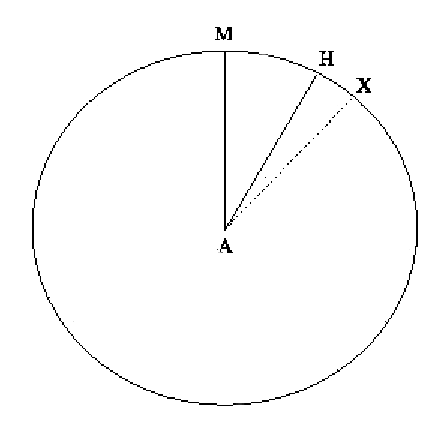
\includegraphics[scale=0.75]{fig1.eps}\\
\caption{}
\end{figure}
\begin{figure}[htbp]
\centering 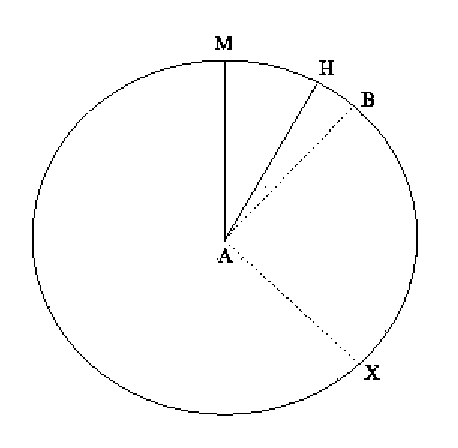
\includegraphics[scale=0.75]{fig2.eps}\\
\caption{}
\end{figure}
\begin{figure}[htbp]
\centering 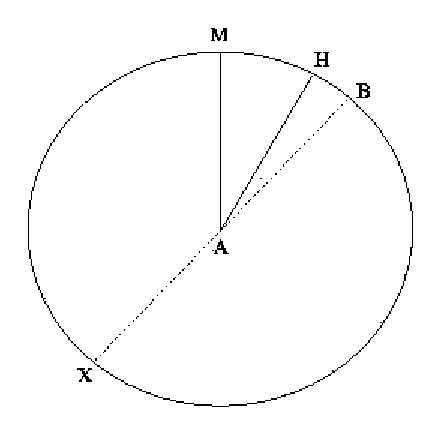
\includegraphics[scale=0.75]{fig3.eps}\\
\caption{}
\end{figure}

(1) Let $AM$ and $AH$ in all the figures denote the positions
of the minute and hour hands at 1 o'clock, and $AX$
(Fig. 1) the position of both hands when together.

\[
\begin{array}{rrcl}
\text{Let}\qquad & x &=& \text{number of minute spaces in arc } MX.\\
  &MX &=& MH + HX.   \\
  & x &=& 5 + \frac{x}{12}. \text{  Solution gives } x=5\frac{5}{11}.
\end{array}
\]

Hence, the time is $5\frac{5}{11}$ minutes past 1 o'clock.

(2) Let $AX$ and $AB$ (Fig. 2) denote the positions of
the minute and hour hands when at right angles.
\[
\begin{array}{rrcl}
\text{Let } & x &=& \text{ number of minute spaces in arc } MBX.  \\
 & MBX &=& MH + HB + BX.   \\
&x &=&5 + \frac{x}{12} + 15.\text{ Solution gives } x=21\frac{9}{11}.
\end{array}
\]

Hence, the time is $21\frac{9}{11}$ minutes past 1 o'clock.

(3) Let $AX$ and $AB$ (Fig. 3) denote the positions of
the minute and hour hands when opposite.


\begin{tabular}{rrcl}
Let &  $x$ &=& number of minute spaces in arc $MBX$.   \\
    &$MBX$ &=& $MH +HB + BX.$   \\
    &  $x$ &=& $5+\frac{x}{12}+30$. Solution gives $x=38\frac{2}{11}$.
\end{tabular}


Hence, the time is $38\frac{2}{11}$ minutes past 1 o'clock.

\item At what time are the hands of a clock together
between 2 and 3? Between 5 and 6? Between 9 and 10?

\item At what time are the hands of a clock at right
angles between 2 and 3? Between 4 and 5? Between 7
and 8?

\item At what time are the hands of a clock opposite each
other between 3 and 4? Between 8 and 9? Between 12
and 1?

\item At what times between 4 and 5 o'clock are the hands
of a watch ten minutes apart?

\item At what time between 8 and 9 o'clock are the
hands of a watch 25 minutes apart?

\item At what time between 5 and 6 o'clock is the minute
hand three minutes ahead of the hour hand?

\item It was between 12 and 1 o'clock; but a man, mistaking
the hour hand for the minute hand, thought that
it was 55 minutes later than it really was. What time
was it?

\item At what time between 11 and 12 o'clock are the
hands two minutes apart?

\textit{Illustrative Example}. A courier who travels at the rate
of 6 miles an hour is followed, 5 hours later, by another
who travels at the rate of $8\frac{1}{2}$ miles an hour. In how many
hours will the second overtake the first?
\begin{tabular}{rrcl}
Let &             $x$ &=& number of hours the second is traveling. \\
    &         $x + 5$ &=& number of hours the first is traveling.  \\
    & $8\frac{1}{2}x$ &=& distance the second travels.             \\
    &        $6(x+5)$ &=& distance the first travels.              \\
    & $8\frac{1}{2}x$ &=& $6 (x + 5)$. Solution gives $x=12$.      \\
\multicolumn{4}{l}{He will overtake the first in 12 hours.}
\end{tabular}

\item A messenger who travels at the rate of 10 miles an
hour is followed, 4 hours later, by another who travels at
the rate of 12 miles an hour. How long will it take the
second to overtake the first?

\item A courier who travels at the rate of 19 miles in 4 hours
is followed, 8 hours later, by another who travels at the rate
of 19 miles in 3 hours. In what time will the second
overtake the first? How far will the first have gone
before he is overtaken?

\item A train going at the rate of 20 miles an hour is
followed, on a parallel track, 4 hours later, by an express
train. The express overtakes the first train in $5\frac{1}{3}$ hours.
What is the rate of the express train?

\item A messenger started for Washington at the rate of
$6\frac{1}{2}$ miles an hour. Six hours later a second messenger
followed and in $4\frac{7}{8}$ hours overtook the first just as he was
entering the city. At what rate did the second messenger
go? How far was it to Washington?

\item How far could a man ride at the rate of 8 miles an
hour so as to walk back at the rate of 4 miles an hour and
be gone only 9 hours?

\item Two persons start at 10 A.M. from towns A and B,
$55\frac{1}{2}$ miles apart. The one starting from A walks at the
rate of $4\frac{1}{4}$ miles an hour, but stops 2 hours on the way;
the other walks at the rate of $3\frac{3}{4}$ miles an hour without
stopping. When will they meet? How far will each
have traveled?

\textit{ Suggestion}. Let x equal the number of hours.

\item A boy who runs at the rate of $12\frac{1}{2}$ yards per second,
starts 16 yards behind another whose rate is 11 yards per
second. How soon will the first boy be 8 yards ahead of
the second?

\item A rectangle whose length is 4 ft. more than its
width would have its area increased 56 sq. ft. if its length
and width were each made 2 ft. more. What are its
dimensions?

\item The length of a room is double its width. If the
length were 3 ft. less and the width 3 ft. more, the area
would be increased 27 sq. ft. Find the dimensions of the
room.

\item A floor is two-thirds as wide as it is long. If the
width were 2 ft. more and the length 4 ft. less, the area
would be diminished 22 sq. ft. What are its dimensions?

\item A rectangle has its length and width respectively
4 ft. longer and 2 ft. shorter than the side of an equivalent
square. Find its area.

\item An enclosed garden is 24 ft. greater in length than in
width. 684 sq. ft. is used for a walk 3 ft. wide extending
around the garden inside the fence. How long is the
garden?

\item Factor $\displaystyle \frac{x^2}{4}-\frac{y^2z^4}{9m^6}$,
$x^6-27y^3$, $a^{16}-b^{16}$, $2c-4c^3+2c^5$.

\item Extract the square root of $12x^4-24x+9+x^6-22x^3-4x^5+28x^2$.

\item What must be subtracted from the sum of
$4x^3+3x^2y-y^3$, $4x^2y-3x^3$, $7x^2y+9y^3-2x^2y$, to leave the remainder
$2x^3-3x^2y+y^3$?

\item Find the G.C.F. of $x\left(x+1\right)^2$, $x^2(x^2-1)$, and
$2x^3-2x^2-4x$.

\item From one end of a line I cut off 5 feet less than one-fifth
of it, and from the other end 4 feet more than one-fourth of it,
and then there remained 34 feet. How long was the line?

\item A can do twice as much work as B, B can do twice
as much as C, and together they can complete a piece of
work in 4 days. In what time can each alone complete the
work.

\item Separate 57 into two parts, such that one divided by
the other may give 5 as a quotient, with 3 as a remainder.

\item Divide 92 into two parts, such that one divided by
the other may give 4 as a quotient, with 2 as a remainder.

\item Fourteen persons engaged a yacht, but before sailing,
four of the company withdrew, by which the expense
of each was increased \$4. What was paid for the yacht?

\item Find two consecutive numbers such that a fifth of
the larger shall equal the difference between a third and an
eighth of the smaller.

\item A is 24 years older than B, and A's age is as much
above 50 as B's is below 40. What is the age of each?

\item Find the number, whose double added to 16 will
be as much above 70 as the number itself is below 60.

\item A hare takes 5 leaps to a dog's 4, but 3 of the dog's
leaps are equal to 4 of the hare's; the hare has a start of
20 leaps. How many leaps will the hare take before he is
caught?

\textit{ Suggestion}. Let $5x$ equal the number of leaps the hare
will take, and let $m$ equal the length of one leap.

\item A greyhound takes 3 leaps to a hare's 5, but 2 of
the greyhound's leaps are equal to 4 of the hare's. If the
hare has a start of 48 leaps, how soon will the greyhound
overtake him?

\item A hare has 40 leaps the start of a dog. When will
he be caught if 5 of his leaps are equal to 4 of the dog's,
and if he takes 7 leaps while the dog takes 6?
\end{enumerate}


\section*{SIMULTANEOUS EQUATIONS.}
\addcontentsline{toc}{section}{\numberline{}SIMULTANEOUS.}

\[
\textbf{48. } \textrm{ILLUS. } \left. \begin{array}{cc} x + y = 8, & x=3\\
4x-y=7, & y=5 \end{array} \right\} \textrm{ in both equations. }
\]

\textbf{Simultaneous equations} are equations in which the
same unknown numbers have the same value.

One equation containing more than one unknown
number cannot be solved. There must be as many
simultaneous equations as there are unknown numbers.

\[
 \textrm{ILLUS. 1.  Solve} \left\{ \begin{array}{c} x + 3y = 17,\\
2x+y=9. \end{array} \right.
\]

Multiply the first equation by 2;

\[
 \left. \begin{array}{cc} \textrm{then} & 2x + 6y = 34, \\
\textrm{but} & \underline{2x+y=9}\\
\textrm{  Subtracting, } & 5y=25\\
& y=5. \end{array} \right.
\]

To find the value of $x$, substitute the value of $y$ in the
second equation:

\[
2x + 5 = 9, 2x = 4, x = 2.
\]

\[
 Ans. \left\{ \begin{array}{l} x = 2,\\
y=5 \end{array} \right.
\]

\[
 \textrm{ILLUS. 2.  Solve} \left\{ \begin{array}{c} 3x + 4y = 12,\\
5x - 6y=1. \end{array} \right.
\]

Multiply the first equation by 3, and the second equation
by 2,

\[ \begin{array}{l rrr l}
                &  9x & {}+ 12y = & 36   \\
                & 10x & {}- 12y = &  2   \\
\cline{2-4} \text{Adding, } & 19x &           & 38 & \therefore x
= 2.
\end{array}
\]

Substituting, $6 + 4y = 12$, $4y = 6$, $y = 1\frac{1}{2}$.

\textit{Multiply one or both of the equations by such a number
that one of the unknown numbers shall have like coefficients. If
the signs of the terms having like coefficients are alike,
subtract one equation from the other; if unlike, add the
equations}.

\subsubsection*{Exercise 55.}
Solve: \begin{enumerate} \item
$
 \left\{ \begin{array}{rcrcl}
 x &+&  y &=& 4,   \\
3x &-& 2y &=& 7 .
\end{array} \right.
$
\item
$
\left\{ \begin{array}{rcrcl}
 x &-&  y &=& 2,   \\
2x &+& 5y &=& 18 .
\end{array} \right.
$
\item
$
\left\{ \begin{array}{rcrcl}
5x &+& 2y &=& 47,   \\
2x &-&  y &=& 8 .
\end{array} \right.
$
\item
$
 \left\{ \begin{array}{rcrcl}
4x &-& 3y &=& 10,   \\
6x &+& 4y &=& 49 .
\end{array} \right.
$
\item
$
 \left\{ \begin{array}{rcrcl}
  8x &-& 2y &=& 6,   \\
 10x &+& 7y &=& 36 .
\end{array} \right.
$
\item
$
 \left\{ \begin{array}{rcrcl}
 2x &-& 5y &=& -11,   \\
 3x &+&  y &=& 9 .
\end{array} \right.
$
\item
$
\left\{ \begin{array}{rcrcl}
 7x &-& 3y &=& 41,   \\
 2x &+&  y &=& 12 .
\end{array} \right.
$ \item
$
 \left\{ \begin{array}{rcrcl}
 2x &+&  9y &=& -5,   \\
11x &+& 15y &=& 7 .
\end{array} \right.
$
\item
$
\left\{ \begin{array}{rcrcl}
 4y &-& 2x &=& 4,   \\
10y &+& 3x &=& -8 .
\end{array} \right.
$
\item
$
 \left\{ \begin{array}{rcrcl}
3x &-& 5y &=& 15,   \\
5x &+& 3y &=& 8 .
\end{array} \right.
$
\item
$
\left\{ \begin{array}{rcrcl}
3y &-& 2x &=& 3,   \\
4y &-& 6x &=& 2\frac{1}{3} .
\end{array} \right.
$
\item
$
\left\{ \begin{array}{rcrcl}
3x &+ & 2y &=& 11,\\
 7x &-& 5y &=& 190.
\end{array} \right.
$
\item
$
\left\{ \begin{array}{rcrcl}
\frac{1}{2}x &+& \frac{1}{3}y &=& 11,\\
          8x &+& \frac{2}{5}y &=& 102.
\end{array} \right.
$
\item
$
\left\{ \begin{array}{rcrcl}
         5x &+&           2y &=& 66,\\
\frac{x}{3} &+& \frac{3y}{4} &=& 15\frac{1}{2}.
\end{array} \right.
$

\item $\left\{ \begin{matrix}\frac{3x}{5} - \frac{2y}{7} = 35, \\ x + 2y = -63.\end{matrix}\right.$

\item $ \left\{ \begin{matrix}x - \frac{3y}{5} = 6,
\\ \frac{2x}{3} + 7y = 189.\end{matrix}\right.$

\item $\left\{ \begin{matrix}\frac{x + 2y}{3x - y} = 1, \\
\frac{4y - x}{3 + x - 2y} = 2\frac{1}{2}.\end{matrix}\right.$

\item $\left\{ \begin{matrix}\frac{x + 2y}{x - 2} = -5\frac{2}{3},
\\ \frac{2y - 4x}{3 - y} = -6.\end{matrix}\right.$

\item $\left\{ \begin{matrix}y - \frac{2y + x}{3} = \frac{2x + y}{4} - 8\frac{3}{4}, \\ \frac{3x + y}{2} - \frac{y}{3} = \frac{109}{10} + \frac{4y - x}{5}.\end{matrix}\right.$

\item $\left\{ \begin{matrix}x + y = a, \\ x - y = b.\end{matrix}\right.$

\item $\left\{ \begin{matrix}\frac{3x - 19}{2} + 4 = \frac{3y + x}{3} + \frac{5x - 3}{2}, \\ \frac{4x + 5y}{16} + \frac{2x + y}{2} = \frac{9x - 7}{8} + \frac{3y + 9}{4}.\end{matrix}\right.$

\item $\left\{ \begin{matrix}\frac{1}{5}(3x - 2y) + \frac{1}{3}(5x - 3y) = x, \\ \frac{4x - 3y}{2} + \frac{2}{3}x - y = 1 + y.\end{matrix}\right.$

\item If 1 is added to the numerator of a fraction, its
value is $\frac{1}{8}$; but if 4 is added to its denominator, its value
is $\frac{1}{4}$. What is the fraction?

\textit{ Suggestion}. Letting $x$ equal the numerator, and $y$ the
denominator, form two equations.

\item If 2 is subtracted from both numerator and denominator
of a certain fraction, its value is $\frac{3}{5}$; and if 1 is
added to both numerator and denominator, its value is $\frac{2}{3}$.
What is the fraction?

\item If 2 is added to both numerator and denominator of
a certain fraction, its value is $\frac{2}{3}$; but if 3 is subtracted
from both numerator and denominator, its value is $\frac{1}{2}$.
What is the fraction?

\item If 3 be subtracted from the numerator of a certain
fraction, and 3 be added to the denominator, its value will
be $\frac{1}{2}$; but if 5 be added to the numerator, and 5 be subtracted
from its denominator, its value will be 2. What is
the fraction?

\item The sum of two numbers divided by 2 is 43, and
their difference divided by 2 is 19. What are the numbers?

\item The sum of two numbers divided by 3 gives as a
quotient 30, and their difference divided by 9 gives 4.
What are the numbers?

\item Five years ago the age of a father was four times
that of his son; five years hence the age of the father will
be $2\frac{1}{3}$ times that of the son. What are their ages?

\item Seven years ago John was one-half as old as Henry,
but five years hence he will be three-quarters as old.
How old is each?

\item $A$ and $B$ own herds of cows. If $A$ should sell 6
cows, and $B$ should buy 6, they would have the same number;
if $B$ should sell 4 cows to $A$, he would have only
half as many as A. How many cows are there in each
herd?

\item The cost of 5 pounds of tea and 7 pounds of coffee is
\$4.94; the cost of 3 pounds of tea and 6 pounds of coffee is
\$3.54. What is the cost of the tea and coffee per pound?

\item What is the price of corn and oats when 4 bushels of corn
with 6 bushels of oats cost \$4.66, and 5 bushels of corn with 9
bushels of oats cost \$6.38?

\item A merchant mixes tea which cost him 87 cents a pound with
tea which cost him 29 cents a pound. The cost of the mixture is
\$17.98. He sells the mixture at 55 cents a pound and gains
\$2.92. How many pounds of each did he put into the mixture?
\end{enumerate}



\subsection*{QUADRATIC EQUATIONS.}
\addcontentsline{toc}{section}{\numberline{}QUADRATIC.}

\begin{tabular}{llc} \textbf{ 49}. &ILLUS. 1.& $ax^2 = b$, $7x^2-10 =
5+2x^3$.\\
& ILLUS. 2. &$x^2+8x = 20$, $ax^2+bx-c = bx^2+d$.
\end{tabular}

A \textbf{ quadratic equation} is an equation in which, the
highest power of the unknown number is a square. It is called an
equation of the second degree.

If it contains only the second power of the unknown number (Illus.
1), it is called a \textbf{ pure quadratic equation}. If it
contains both the first and second powers of the unknown number
(Illus. 2), it is called an \textbf{ affected quadratic equation}.

\textbf{ 50}. ILLUS. Solve $x^2-\frac{x^2-10}{3} =
35-\frac{x^2+50}{5}$.
\begin{align}
15x^2-5x^2+50 &= 525-3x^2-150.\\
        13x^2 &= 325.\\
          x^2 &= 25.\\
            x &= {\pm}5.
\end{align}

\textit{ To solve a pure quadratic equation, reduce to the form
$x^2 = a$ and take the square root of each member}.

\subsubsection*{Exercise 56}.

Solve:
\begin{enumerate}
\item $5x^2-12 = 33$.

\item $3x^2+4 = 16$.

\item $4x^2+ll = 136-x^2$.

\item $5(3x^2-1) = 11(x^2+1)$.

\item $\displaystyle \frac{2}{5x^2}-\frac{1}{3x^2} =
\frac{4}{15}$.

\item $\displaystyle \frac{x^2-1}{6}+\frac{1}{4} =
\frac{x^2+1}{8}$.

\item $(x+3)^2 = 6x+58$.

\item $\displaystyle 6x+2+\frac{16}{x} =
\frac{15+40x}{4}-1\frac{3}{4}$.

\item $\displaystyle
\frac{x-3}{x-1}+\frac{x+1}{x+3}+\frac{8}{x^2+2x-3} = 0$.

\item $\displaystyle \frac{x+1}{x-1}+\frac{2(x-3)}{x-2} =
\frac{16-9x}{x^2-3x+2}$.

\item $\displaystyle
\frac{1}{(2-x)(3-x)}-\frac{2}{(1-x)(x-3)}+\frac{1}{(x-1)(x-2)} =
\frac{1}{2-x}+\frac{1}{(x-1)(2-x)(x-3)}$.

\item $\displaystyle
\frac{1}{6x+6}-\frac{1}{2x+2}+\frac{10}{3-3x^2} =
\frac{x}{3(1-x)}$.

\item A father is 30 years old, and his son is two years
old. In how many years will the father be three times as
old as his son?

\item Divide the number 112 into two parts such that the
smaller divided by their difference will give as a quotient
3.

\item The numerator of a fraction is 4 less than the denominator;
if 30 be added to the denominator, or if 10 be subtracted
from the numerator, the resulting fractions will
be equal. What is the original fraction?

\end{enumerate}
\textbf{ 51.} ILLUS. Solve
$\frac{x-1}{x-2}-\frac{x-3}{x-4}=-\frac{2}{3}$.

\begin{eqnarray*}
3x^2-15x+12-3x^2+15x-18 & = & -2x^2+12x-16. \\
2x^2-12x & = & -10. \\
x^2-6x & = & -5. \\
x^2-6x-5 & = & 0. \\
(x-5)(x-1) & = & 0. \\
\end{eqnarray*}

This equation will be satisfied if either factor is equal
to zero. Placing each factor in turn equal to zero, and
solving,

\begin{tabular}{rclrcl}
x-5 & = & 0, & x-1 & = & 0, \\
x   & = & 5; & x   & = & 1. \\
\end{tabular}

\textit{ Ans.} $x=5$ or $1$.

\textit{ To solve an affected quadratic equation, reduce the
equation to the form $x^2 + bx + c = O$, factor the first member,
place each factor in turn equal to zero, and solve the simple
equations thus formed.}

\subsubsection*{Exercise 57.}

Solve:

\begin{enumerate}
\item $x^{2}+3x=18$.
\item $x^{2}+5x=14$.
\item $x(x-1)=72$.
\item $x^{2}=10x-21$.
\item $23x=120+x^{2}$.
\item $187=x^{2}+6x$.
\item $x^{2}-2bx=-b^{2}$.
\item $x^{2}=4ax-3a^{2}$.
\item $x^{2}+(a-1)x=a$.
\item $adx-acx^{2}=bcx-bd$.
\item $(x+3)(x-3)=8(x+3)$.
\item $(x+2)(x-5)=4(x-4)$.

\item $\displaystyle \frac{x}{5}+\frac{2}{x}=1\frac{2}{5}$.

\item $\displaystyle \frac{x}{3}-2=\frac{x^{2}}{12}-\frac{x}{2}$.

\item $\displaystyle \frac{8}{x-2}-3+\frac{x+1}{7}=0$.

\item $\displaystyle \frac{x}{x+1}-2\frac{1}{6}+\frac{x+1}{x}=0$.

\item $\displaystyle x+4=3x-\frac{24}{x-1}$.

\item $\displaystyle
\frac{x-1}{x+1}+\frac{x+3}{x-3}=\frac{2(x+2)}{x-2}$.

\item $\displaystyle
\frac{x-1}{x+2}-\frac{3x^{2}+2}{x^{2}-4}=\frac{3x}{2-x}$.

\item $\displaystyle
\frac{2x}{3-x}+\frac{2x(x-3)}{x^2-9}=\frac{x-3}{x+3}$.

\item At what time between 4 and 5 o'clock are the hands of a
clock opposite each other?

\item John, having three times as much money as Lewis, gave Lewis
\$2, and then had twice as much as Lewis. How much had each at
first?

\item A fish is 3 feet long; its head is equal in length to the
tail, and its body is five times the length of the head and tail
together. What is the length of the head?

\item In how many days can A, B, and C build a boat
if they work together, provided A alone can build it in
24 days, B in 18 days, and C in 30 days?

\end{enumerate}

The above method of solving affected quadratic equations is the
simplest of three methods commonly used, and will not solve all
possible cases; the method given for solving simultaneous
equations is only one of three known methods; the cases in
factoring are less than half of those usually taken. In fact, we
have made only a beginning in the subject of algebra; much more
lies ahead along the lines which we have been following. \textit{
Can you grasp more clearly the conditions given in any problem
presented to you, and see more definitely just what is required,
than when you began this study? Do you possess greater ability to
think out problems? Has the use of letters to represent numbers
made you think more exactly what is to be done, and what the
operations mean?} If so, your knowledge of numbers is broader, and
you already know that

\textbf{ \textit{ Algebra is the knowledge which has for its
object general truths about numbers.}}

\subsubsection*{Exercise 58. (General Review.)}
\begin{enumerate}
\item When $a=l$, $b = 3$, $c = 5$, and $d = O$, what is the
value of

$\displaystyle
\frac{4a+b^2+b^2c^2+ad}{b^2+c^2+d^2}-\frac{1+a^2c^2}{a^2+c^2+d^2}
+\frac{a^2+b^2+d^2}{1+a^2b^2+bd}-\frac{a^2+2ab+b^2}{b^2-2bc+c^2}$?

\item Prove that $\displaystyle
(x^{2}+xy+y^{2})(x^{2}-xy+y^2)=\frac{x^{6}-y^{6}}{x^{2}-y^{2}}$

\item Solve $(x+5)^{2}-(x+1)^{2}-16x=(x-1)^{2}-(x-5)^{2}$.

\item A tank is filled by two pipes, $A$ and $B$, running
together, in 12 hours, and by the pipe $B$ alone in 20 hours.
In what time will the pipe $A$ alone fill it?

\item Find the G.C.F. of  $x^{3}+1-x-x^{2}$, $x^{3}+x-1-x^{2}$,
$x^{4}-1$, and $x^{2}-4x+3$.

\item Divide $a^{5}+a^{4}b-a^{3}b^{2}+a^{3}-2ab^{2}+b^{3}$ by $a^{3}-b+a$.

\item Find the square root of $5y^{4}+1+12y^{5}-2y-2y^{3}+4y^{6}+7y^{2}$.

\item Expand
\[
(x+1)(x+2)-(2x+1)(2x+3)+(x-4)(x-9)+(x-5)^{2}.
\]

\item Solve $\displaystyle
\frac{x+2}{x-2}+\frac{x-2}{x+2}=\frac{5}{2}$.

\item Simplify

\[
\left(\frac{1}{x-1}-\frac{3}{(x+3)(x-1)}\right)\div\left(\frac{1}{x+3}+\frac{1}{(x-1)(x+3)}\right).
\]

\subsection*{II.}

\item Add $2(a-c)^{3}-10x^{3}y-7(a-c)$, $6(a-c)-2(a-c)^{3}-10x^{3}y$,
$3(a-c)-(a-c)^{3}+2x^{3}y$, $2(a-c)+x^{3}y-(a-c)^{3}$,
$4(a-c)+5(a-c)^3+2x^{3}y$, $3(a-c)-2x^{3}y-6(a-c)^3$.

\item Solve $bx-b^{2}=3b^{2}-4bx$.

\item Factor $x^{6}+2x^{3}-3$, $ax^{2}-ay^{2}+by^{2}-bx^{2}$, $27x^3+(y+z)^{3}$.

\item Find the fraction which becomes equal to one when
six is added to the numerator, and equal to one-third when
four is added to the denominator.

\item Simplify $\displaystyle \frac{ \frac{a^2}{b^3} + \frac{1}{a}
}
                   { \frac{a}{b^3} - \frac{1}{b} + \frac{1}{ab} }$.

\item Solve $\displaystyle
\frac{7x+9}{4}=\left(x-\frac{2x-1}{9}\right)+7$.

\item Six years ago John was five times as old as Sarah.
If he is twice as old as Sarah now, what are their ages?

\item Multiply together $\frac{1-x^2}{1+y}$, $\frac{1-y^2}{x+x^2}$, and $1+\frac{x}{1-x}$.

\item Simplify
$a^2 - (b^2-c^2) - \{b^2 - (c^2-a^2)\} + \{c^2 - (b^2-a^2)\}$.

\item $x$ times $y$ is how many times $a$?


\subsection*{III.}

\item Add $2x + y - 2a + 55\frac{1}{2}b$, $24b-y + 2x + a$, $3a -
2y - 4x - 81b$, and subtract the result from $2y + 3a +
\frac{1}{2}b + 3x$.

\item Divide $\frac{11}{8}a^2-\frac{5}{4}a^3-\frac{1}{2}a+a^4$ by $a^2-\frac{1}{2}a$.

\item A can do a piece of work in 3 days which B can do
in 5 days. In what time can they do it working together?

\item Simplify $\displaystyle \frac{a-b}{a^2-ab+b^2}
 + \frac{ab}{a^3+b^3} + \frac{1}{a+b}$.

\item Factor $x^2-9x-52$, $1-a^{16}$, $(a^2 + b^2)^2 + 2(a^4-b^4) + (a^2-b^2)^2$.

\item Solve $\displaystyle \frac{3x}{4} - \frac{x-10}{2} = x -6
-\frac{x-4}{2}$.

\item The sum of the ages of a man and his son is 100
years; one-tenth of the product of their ages exceeds the
father's age by 180. How old are they?

\item Solve $x = 9 - \frac{y}{2}$, $y = 11 + \frac{x}{3}$.

\item From what must $3x^4 - 2x^3 + x - 6$ be subtracted
to produce unity?

\item Find the following roots: $\sqrt{5.5225}$, $\sqrt[3]{32.768}$.

\subsection*{IV.}

\item Find the value of $\displaystyle \frac{4x^3+2y^3}{ab} +
\frac{2y^3 + 4z^3}{z^3+y^2} - \frac{b^3-z^2b}{a^2 b}$, if $x=1$,
$y = 2$, $z = 0$, $a = 4$, and $b = 5$.

\item Solve $\displaystyle \frac{4}{x-6} - \frac{3}{x-9} =
\frac{1}{x-3}$.

\item Find three consecutive numbers whose sum is 78.

\item Find the G.C.F. of $2a^3 - 12a - 2a^2$, $a^4 - 4a^2$ and
$4a^3b + 16ab + 16a^2b$.

\item Divide $\displaystyle \frac{x^4 - y^4}{x^2 - 2xy + y^2}$ by
$\frac{x^2 + xy}{x-y}$.

\item A fraction becomes $\frac{3}{4}$ by the addition of three to the
numerator and one to the denominator. If one is subtracted
from the numerator and three from the denominator, it becomes
$\frac{1}{2}$. What is the fraction?

\item Expand
$\left(\frac{3a^2b\left(m+n\right)^2}{4xy^3}\left(a-b\right)^3\right)^3$,
$\sqrt{\frac{50x^4\left(a+b\right)^7}{32y^6z^2(a+b)}}$.

\item If a certain number is multiplied by itself, the result is
$9x^4 - 4x + 10x^2 + 1 - 12x^3$. Find the number.

\item Simplify $\displaystyle \frac{ax-x^2}{\left(a+x\right)^2}
\times \frac{a^2+ax}{\left(a-x\right)^2} \div
\frac{2ax}{a^2-x^2}$.

\item Solve $18x-20y = 3$, $\displaystyle
\frac{4y-2}{3}-\frac{5x}{2}= 0$.

\subsection*{V.}

\item Factor $x^4+5x^2+6$, $x^2-14x+49$, $x^2-\left(y+z\right)^2$.

\item Add $xy-\frac{9}{8}x-\frac{7}{12}(x^2-y^2)-5x^2y^2$, $\frac{5}{8}x-xy+9x^2y^2
+\frac{2}{3}(x^2-y^2)$, $\frac{1}{9}x^2y^2-xy+\frac{1}{4}x+\frac{3}{4}(x^2-y^2)$, $2xy+\frac{1}{4}x
-\frac{5}{6}(x^2-y^2)-4x^2y^2$.

\item At what times between 7 and 8 o'clock are the
hands of a clock six minutes apart?

\item Simplify $\displaystyle \frac{x^2-5x+6}{x^2-2x+1} \times
\frac{x^2-4x+3}{x^2-4x+4} \div \frac{x^2-6x+9}{x^2-3x+2}$.

\item Solve $\displaystyle \frac{x+2}{b+2}=2-\frac{x+1}{b+1}$.

\item Factor $\displaystyle \frac{x^6}{y^6}-\frac{a^2b^4}{c^2}$,
$\displaystyle \frac{x^2}{y^2}-\frac{5x}{y}-14$, $\displaystyle
\frac{x^2}{y^2}-2+\frac{y^2}{x^2}$.

\item A, who works only two-thirds as fast as B, can
build a stone wall in 12 days. In what time could A
and B together build the wall?

\item Solve $\displaystyle \frac{x+y}{2}-\frac{x-y}{3}=8$,
$\frac{x+y}{3}+\frac{x-y}{4}=11$.

\item Expand $\left(1+2x\right)^3$, $\left(2x^2-3a^2b^3\right)^4$.

\item Reduce $\displaystyle
\frac{(a^4+2a^2b^2+b^4)(a^4+b^4)}{a^8-b^8}$ to lowest terms.

\subsection*{VI.}

\item $y$ is how much greater than $x$?

\item Subtract $3x^3+4x^2y-7xy^2+10y^3$ from $4x^3-2x^2y
+4xy^2+4y^3$ and find the value of the remainder when
$x=2$ and $y=1$.

\item The length and width of a rectangle are respectively
5 feet longer and 4 feet.shorter than the side of an equivalent
square. What is its area?

\item Find the L.C.M. of $a^2-3-2a$, $a^2-1$, and $2a^2
-6a + 4$.

\item Simplify $\displaystyle
\frac{\frac{b}{4a}-1+\frac{a}{b}}{\frac{b}{2a}-\frac{2a}{b}}$.

\item Solve $\displaystyle \frac{x-1}{3}+\frac{3}{x-1}=2$.

\item Factor $a^4b+8ac^3bm^6$, $4c^3x^2+cy^2+4c^2xy$, $x^6-1$.

\item Multiply $\displaystyle
1-\frac{1}{2}x-\frac{1}{3}x^2+\frac{1}{4}x^3$ by
$1-\frac{1}{3}x^2-\frac{1}{4}x^3-\frac{1}{2}x$.

\item Find the cube root of $6x^4+7x^3+3x^5+6x^2+x^6+1+3x$.

\item Divide $12x^2y^2- 4y^4 - 6x^3y + x^4$ by $x^2+2y^2-3xy$.

\subsection*{VII.}

\item Add $\frac{1}{10}a^3-\frac{4}{5}a^4-\frac{1}{5}a^2+\frac{3}{10}a$, $\frac{1}{4}a^2-\frac{4}{5}a-\frac{5}{7}a^4-\frac{1}{8}a^3$,
$\frac{5}{7}a^4+\frac{1}{8}a^3+\frac{3}{4}a^2+\frac{2}{5}a$, $\frac{4}{5}a^4+\frac{1}{5}a^2+\frac{2}{5}a^3+\frac{1}{10}a$.

\item Solve $x(a-x)+x(b-x)=2(x-a)(b-x)$.

\item Factor $x^4-22x^2-75$, $16-x^8$, $\left(a+b\right)^2-\left(a-b\right)^2$.

\item A piece of work can be finished by 3 men in 8 days,
or by 5 women in 6 days, or by 6 boys in 6 days. In what
time can 2 men, 3 women, and 3 boys do the work?

\item Solve $\displaystyle
\frac{3x+19}{2}-\left(\frac{x+1}{6}+3\right)=\frac{5x+2}{3}-\left(3-\frac{3x-1}{2}\right)$.

\item Expand $\displaystyle
\left(\frac{a}{b}-\frac{c}{d}\right)^3$, $\displaystyle
\left(\frac{c}{d}+1\right)\left(\frac{c^2}{d^2}-\frac{c}{d}+1\right)$.

\item What number is that, the sum of whose third and
fourth parts is less by two than the square of its sixth part?

\item Solve $\displaystyle \frac{x}{5}-\frac{y}{7}=1$,
$\frac{2x}{3}-\frac{y}{2}=3$.

\item Divide $m$ by $1+y$ to four terms.

\item If $x$ is $\frac{3}{5}$ of a number, what is the number?


\subsection*{VIII.}

\item The head of a fish is 6 inches long, the tail is
as long as the head and half the body, and the body is
as long as the head and tail. What is the length of the
fish?

\item Add $4a - 5x - 15y$, $a + 18x + 8y$, $4a - 7x+11y$,
$a+3x+5y$, and multiply the result by the difference between $11a
+ 7y$ and $10a +6y - x$.

\item Divide $2x^2+\frac{9}{2}x^4+\frac{8}{9}$ by $2x+3x^2+\frac{4}{3}$.

\item How many numbers each equal to $1-2x+x^2$ must
be added together to equal $5x^6-6x^5+1$?

\item Factor $a^3+5a^2-4a-20$, $x^6-y^6$, $2x^5-8x^3y^2+6xy^4$.

\item A courier who travels at the rate of 5 miles an hour
is followed, 4 hours later, by another who travels at the rate
of 15 miles in 2 hours. In how many hours will the
second overtake the first?

\item Divide $\displaystyle \frac{1}{1-x}-\frac{1}{1+x}$ by
$\displaystyle \frac{1}{1-x}+\frac{1}{1+x}$.

\item Solve $3x-4y=-6$, $10x+2y=26$.

\item $3xy-3a^2+4b^2-5cd+4xy-6a^2-7b^2+7cd+3xy
-6a^2+6b^2-3cd-5xy+7a^2-6b^2+4cd+4xy+7a^2
-7b^2+4cd-6xy-6a^2+3b^2-7cd+7a^2=?$

\item Simplify
$3x-5-\{2(4-x)-3(x-2)\}+\{3-(5+2x)-2\}$.
\end{enumerate}

\chapter*{ANSWERS TO A FIRST BOOK IN ALGEBRA.}


\subsection*{Exercise 1.}

\begin{enumerate} \item 43; 86.

\item Carriage, \$375; horse, \$125.

\item C, \$31; J, \$155.

\item 8; 56.

\item 8 miles.

\item Needles, 8�; thread, 64�.

\item 224 girls; 448 boys.

\item 25; 275.

\item H, 6 qts.; J, 18 qts.

\item Lot, \$720; house, \$3600.

\item Mr. A, 72; son, 24.

\item 50 A.; 300 A.

\item Dict., \$7.20; rhet, \$.90.

\item 112; 4144.

\item Aleck, 56�; Arthur, 8�.

\item Mother, 28; daughter, 4.

\item J, 15 yrs.; M, 5 yrs.

\end{enumerate}

\subsection*{Exercise 2.}
\begin{enumerate}

 \item Necktie, \$.75; hat, \$3; boots, \$3.75.

\item 30; 45; 15 miles.

\item James, 15; sister, 5; brother, 10.

\item Pig, \$10; cow, \$30; horse, \$50.

\item A, 35; B, 15; C, 5.

\item 12; 48.

\item 8 men; 40 women.

\item Henry, \$200; John, \$400; James, \$800.

\item 4500 ft.; 13,500 ft.; 27,000 ft.

\item 15; 45; 60 pigeons.

\item 165; 33; 11.

\item A, \$44; B, \$11; C, \$55.

\item Calf, \$8; cow, \$16; horse, \$48.

\item 150; 450 gal.

\item Cow, \$30; lamb, \$5.

\item Tea, 90�; coffee, 30�.

\item Mrs. C, \$25,000; Henry, \$5000.
\end{enumerate}

\subsection*{Exercise 3.}

\begin{enumerate}

\item 14 boys; 21 girls.

\item 14 yrs.; 29 yrs.

\item 492; 587 votes.

\item 22; 48.

\item J, 79; H, 64.

\item Flour, 27 bbls.; meal, 30 bbls.

\item 23 Hol.; 40 Jer.

\item \$18; \$26.

\item 40; 59.

\item 16; 19; 21.

\item 21; 17; 24.

\item \$10,000; \$11,500; \$12,700.

\item 21; 38; 6.

\item 51; 28; 16 sheep.

\item A, 253; B, 350; C, 470 votes.

\item 17; 12; 24 A.

\item 36; 20; 55.

\item \$50,000; \$44,000; \$24,000.

\end{enumerate}

\subsection*{Exercise 4.}

\begin{enumerate}
\item C, 34; H, 15.

\item 26 pear; 7 apple.

\item J, 16 qts.; M, 7 qts.

\item 65.

\item 18.

\item 24.

\item 11.

\item Tea, \$8.76; coffee, \$1.63.

\item 15; 33 rooms.

\item 5; 6; 12.

\item 17; 20; 100.

\item \$5000; \$3000; \$10,000.

\item \$50; \$68; \$204.

\item A, \$5000; B, \$10,500; C, \$31,500.

\item 8000; 24,250; 48,500ft.

\item Daughter, \$25,000; son, \$40,000; widow, \$160,000.

\item Father, 14 qts.; older son, 7 qts.; younger son, 4 qts.

\item H, 200 stamps; J, 185 stamps; T, 189 stamps.

\end{enumerate}

\subsection*{Exercise 5.}

\begin{enumerate}

\item Blue, 5 yds.; white, 15 yds.

\item 3.

\item Walked 2 hrs.; rode 8 hrs.

\item Book, \$2; lamp, \$4.

\item 12.

\item 12 twos; 24 fives.

\item Tea, 67�; coffee, 32�.

\item Crackers,18� gingersnaps, 25�

\item Lamp,  \$1; vase, \$1.50.

\item House, \$4500; barn, \$3300.

\item 12,000; 13,500 ft.

\item 29 gal.; 24 gal.

\item Johnson, \$6000; May, \$1500.

\item 27; 10; 42.

\item 3; 17; 51.

\item 3 bbls.; 9 boxes.

\item 18; 90; 180.

\item 84; 132.

\end{enumerate}

\subsection*{Exercise 6.}
\begin{enumerate}
\item 4.

\item 7.

\item 12 yrs.

\item \$6.25.

\item \$8.

\item 8 sheep.

\item 121; 605.

\item 142; 994.

\item \$500; \$1450; \$2900.

\item W, 6 yrs.; J, 9 yrs.

\item 25; 15 marbles.

\item 16.

\item Oranges, 35 cents; apples, 20 cents.

\item 9; 15.

\item 30 yrs.; 32 yrs.

\item Cow, \$30; horse,\$45.

\item 5.

\item Boots, \$5; clothes, \$18.
\end{enumerate}

\subsection*{Exercise 7.}
\begin{enumerate}
\item 14 yrs.; 56 yrs.

\item Corn, 60; wheat, 300.

\item \$3000; \$9000.

\item 70 miles; 35 miles.

\item 45; 720.

\item 189.

\item J, 3 yrs.; M, 15 yrs.

\item 96.

\item \$40,000.

\item 24 marbles.

\item \$30,000.

\item 300 oranges.

\item 90.

\item 60,000ft.

\item 70ft.

\item 72 sq. rds.

\item A, \$22,500; B, \$7500.

\item 30.
\end{enumerate}
\subsection*{Exercise 8.}
\begin{enumerate}
\item 4.

\item 45 marbles.

\item 12; 24; 6 cows.

\item 16.

\item 45.

\item 6048.

\item \$3000.

\item 24.

\item 14.

\item 48,000 ft.

\item 30.

\item 18; 9; 63.

\item 56; 21; 7.

\item 16; 4; 56; 36.

\item Coffee, 18 lbs.; tea, 20 lbs.; cocoa, 24 lbs.

\item \$2500; \$5000; \$7500.

\item J, 9 cents; P, 81 cents.

\item \$12,000.
\end{enumerate}

\subsection*{Exercise 9.}

\begin{enumerate}
 \item 35; 21.

\item 24; 18.

\item 42; 30 miles.

\item 30; 54 yrs.

\item J, 10 boxes; H, 16 boxes.

\item 33 tons; $27\frac{1}{2}$ tons.

\item John, 28yrs.; James, 32yrs.

\item \$1000; \$625.

\item 240 girls; 180 boys.

\item 150 lemons.

\item 21,000 ft.; 6000 ft.

\item 20; 12; 10; l0 miles.

\item 126 cu. yds.

\item M, 390; H, 130.

\item 39; 41; 32; 27.

\item 3205; 2591; 1309.

\item 20 miles; 4 miles; 48 miles.
\end{enumerate}

\subsection*{Exercise 10.}

\begin{enumerate}

\item $x + 9$.

\item $a + p$.

\item $8b$.

\item $x + y$.

\item $c + 5$.

\item $dx$.

\item $m + l + v + c$ dols.

\item $x + y + z$ yrs.

\item $bm$.

\item $d + 1$.

\item $y + z + s$ cts.

\item $m + 1$.

\item $yx$.

\item $x + 40 + a$.

\item $28$; $46$.
\end{enumerate}

\subsection*{Exercise 11.}

\begin{enumerate}
\item $a - b$ or $b - a$.

\item $b - 10$.

\item $a + b - c$.

\item $a -2$, $a - 1$, $a$, $a + 1$, $a + 2$.

\item $a - b$ dols.

\item $c - 8$.

\item $x - 3$, $x - 6$, $x - 9$.

\item $c - b$ dols.

\item $x - 5$.

\item $x$, $x + 9$, or $x$, $x - 9$.

\item $x - 75$ dols.

\item $m + x$ dols.

\item $c - f$ cts.

\item $b - e$ dols.

\item $l + 4 + m - x$ dols.

\item $c - a - b$.

\item $429; 636$ votes.

\item $m + x - y + b - z$ dols.

\item $80 - c$ dols.

\item $x, 60 - x$.
\end{enumerate}

\subsection*{Exercise 12.}

\begin{enumerate}

 \item $2x$.

\item $xyz$.

\item $100x$ cts.

\item $abc$.

\item $ad$ cts.

\item $mb$ miles.

\item $ax$ hills.

\item $x^3$.

\item $a^9$.

\item $d^a$.

\item $3m^3 + a^2$.

\item $x^{2m} + x^m$.

\item $\frac{6}{100}mx$ dols., or $6mx$ cts.

\item $3c - 8$ boys; $4c - 8$ boys and girls.

\item $9x$ days.

\item $3x$ thirds.

\item $5b$ fifths.

\item $m - x + 2a$ dols.

\item $12a - 39$.

\end{enumerate}

\subsection*{Exercise 13.}

\begin{enumerate}
\item $\frac{5a}{3c}$.

\item $\frac{y}{100}$ dols.

\item $\frac{x}{a}$ books.

\item $\frac{m}{y}$ days.

\item $\frac{x}{b}$ dols.

\item $\frac{a + b}{c}$.

\item $a + \frac{b}{c}$.

\item $a + \frac{a}{2}$, or $\frac{3}{2}a$.

\item $300x$.

\item $18b - 3x$ dols.

\item A, $\displaystyle \frac{1}{x}$; B, $\displaystyle
\frac{1}{y}$; C, $\displaystyle \frac{1}{z}$; all, $\displaystyle
\frac{1}{x} + \frac{1}{y} + \frac{1}{z}$.

\item $a^2$ sq. ft.

\item $100a + 10b + 25c$ cts.

\item $\displaystyle \frac{x}{y}$.

\item $\displaystyle \frac{n}{m}$ chestnuts.

\item 12; 18 apples. \end{enumerate}

\subsection*{Exercise 14.} \begin{enumerate}
\setcounter{enumi}{9}

\item 11.

\item 7.

\item 21.

\item 78.

\item 46.

\item $-74$.

\item $-1\frac{1}{3}$.

\item $-4\frac{1}{4}$.

\item 5.

\item 6 apples; 12 pears.

\item 36 years.

\end{enumerate}

\subsection*{Exercise 15.}

\begin{enumerate}
\item $24x$.

\item $25ab$.

\item $-18ax^3$.

\item $-42x$.

\item $10a^2$.

\item $-10abc^2$.

\item $6ab-x^2$.

\item $10ax - 4bc$.

\item $-16a^2$.

\item $8a^4b + 3ab - x^5$.

\item $\frac{3}{2}a$.

\item $-\frac{7}{12}b$.

\item $m + d + c - x$ cts.

\item $a - x - 5 + y$ miles.

\item $5a + 4b + 5c$.

\item $x + y - z$.

\item $-3z - a$.

\item $2x^3 + 4x^2 - 2x + 17$.

\item $a^3 + b^3 + c^3$.

\item $2a^m + 1$.

\item $2a^2b^2c$.

\item $23x^3 - 20x^2 +  27x + 6$.

\item $x^5y + 12x^4y^2 - 16x^3y^3 - 8xy^5$.

\item $5x + 3y + z - a - 3b$.

\item $a^3 + b^3 + c^3 - 3abc$.

\item $mb + c$ men.

\item $x - 10$ cows; $z + 19$ horses.

\item 22 girls; 30 boys. \end{enumerate}

\subsection*{Exercise 16.}

\begin{enumerate}
\item $2a^3$.

\item $12a^2b$.

\item $-9xy^3$.

\item $4x^my$.

\item $8x^2 - 3ax$.

\item $5xy + 7by$.

\item $2a^m$.

\item $9 ax$.

\item $-3a - b + 14c$.

\item $4x - y + 2z$.

\item $8x^4 - 2x^3 + 4x^2 - 15x + 14$.

\item $20a^2b^2 + 16a^2b$.

\item $4x^3 - 2$.

\item $2x^m - x^{2m} - x^{3m}$

\item $2a^{2n} - 18a^nx^n - 9x^{2n}$.

\item $\frac{4}{3}a^2 - \frac{7}{2}a - \frac{1}{2}$.

\item $-2x^4y - 3x^3y^2 + 5xy^4 - y^5$.

\item $x - y + a$.

\item $-3a^2$.

\item $8x^3 - 2x$.

\item $27y^3 - 3z^3 - 6x^3 + 4yz^2 - 11z^2x$.

\item $4x^2 - 16x + 64$.

\item $-4a^2 + 6b^2 - 8bc + 6ab$.

\item $2x^4 - 3x^2 + 2x - 4$.

\item $5a^3 + 2a + 2$.

\item $-11a^2b + 4ab^2 - 12a^2b^2 - b^3$.

\item $b - a$.

\item $x - 3$.

\item $40 - y$ yrs.

\item $\frac{23}{a}$ hrs.
\end{enumerate}
\subsection*{Exercise 17.} \begin{enumerate}

\item $2x + a + b + c - d$.

\item $a + c$.

\item $2a^2b-a^3-2b^3-ab^2$.

\item $3xy - x^2 - 3y^2$.

\item $4b - 4c$.

\item $-2y$.

\item $-6b + 4c$.

\item $-b$.

\setcounter{enumi}{16}

\item $5(x - y)$.

\item $150 - 7(x + y)$.

\item $x + 8$ yrs.

\item $3(x - 35)$ dols.
\end{enumerate}

\subsection*{Exercise 18.} \begin{enumerate}

\item $35 cx$.

\item $-51 acxy$.

\item $21ax^4y^3$.

\item $10a^3b^3c^4$.

\item $18acx^3y^3$.

\item $30a^3b^2c^4$.

\item $-x^3y^3z^3$.

\item $-a^4b^5c^2$.

\item $-\frac{2}{9}a^2cx^6y^4$.

\item $-\frac{3}{20}a^3b^5c^4$.

\item $\frac{100}{ab}$.

\item $100x$.

\item $100a + 10b + c$.

\item $x + 7$ or $x - 7$.
\end{enumerate}

\subsection*{Exercise 19.} \begin{enumerate}

\item $x^4y^2 + x^3y^3 + x^2y^4$.

\item $a^4b - a^3b^2 +a^2b^3$.

\item $-2a^4b + 6a^3b^2 - 2ab^4$.

\item $24x^4y^2 + 108x^3y^3 + 81xy^5$.

\item $a^5b^2 - \frac{6}{25}a^4b^3 - \frac{2}{5}a^3b^4$.

\item $x^3 + y^3$.

\item $x^5 - 4x^4 + 5x^3 - 3x^2 + 2x - 1$.

\item $x^5 + x^4 - 4x^3 + x^2 + x$.

\item $x^2y^2 - 2xy^2n + y^2n^2 - m^2n^2 + 2xm^2n - x^2m^2$.

\item $x^7 + x^6 + 2x^5 + x^2 + x + 2$.

\item $a^6 + b^6$.

\item $x^3 - 3xyz + y^3 + z^3$.

\item $x^7 - y^7$.

\item $x^8 - 8x^4a^4 + 16a^8$.

\item $a^6 + 2a^3y^3 - 9a^4y^4 + y^6$.

\item $x^6 + x^5 + 2x^4 - 11x^3 - 17x^2 - 34x - 12$.

\item $6x^6 - 17x^5 - 12x^4 - 14x^3 + x^2 + 12x + 4$.

\item $5(x + y)$; $4(x - y)$.

\item $\frac{12}{35}$ of the field.

\item $\frac{1}{a} + \frac{1}{b}$.
\end{enumerate}

\subsection*{Exercise 20.} \begin{enumerate}

\item $x^2 + 9x + 14$.

\item $x^2 + 7x + 6$.

\item $x^2 - 7x + 12$.

\item $x^2 - 7x + 10$.

\item $x^2 + 3x - 10$.

\item $x^2 + 4x - 21$.

\item $x^2 - x - 42$.

\item $x^2 - x - 30$.

\item $x^2 - 13x + 22$.

\item $x^2 - 14x + 13$.

\item $y^2 - 2y - 63$.

\item $x^2 + 20x + 51$.

\item $y^2 - 13y - 30$.

\item $y^2 + 18y + 32$.

\item $a^4 + 2a^2 - 35$.

\item  $a^2 - 81$.
\item  $m^4 - 18m^2 + 32$.
\item  $b^6 + 2b^3 - 120$.
\item  $x^2 - \frac{3}{4}x + \frac{1}{8}$.
\item  $y^2 + \frac{1}{2}y + \frac{1}{18}$.
\item  $m^2 + \frac{1}{3}m - \frac{2}{9}$.
\item  $a^2 + \frac{1}{5}a - \frac{6}{25}$.
\item  $x^2 - \frac{7}{6}x + \frac{1}{3}$.
\item  $y^2 + \frac{19}{20}y + \frac{3}{20}$.
\item  $21 - 10x + x^2$.
\item  $15 -8x + x^2$.
\item  $42 - x - x^2$.
\item  $33 + 8x - x^2$.
\item  $x^2 - 9$.
\item  $y^2 - 25$.
\item  $21$.
\item  $12$ cows.
\end{enumerate}


\subsection*{Exercise 21.}

\begin{enumerate}

\item  $a^4b^2$.
\item  $x^3y^6$.
\item  $a^8b^2$.
\item  $-x^9y^6$.
\item  $27 a^6y^3$.
\item  $49 a^2b^4c^6$.
\item  $x^5y^5z^{10}$.
\item  $m^8n^4d^4$.
\item $-125 x^9y^{12}z^3$.
\item  $121 c^{10}d^{24}x^8$.
\item  $\frac{1}{4} x^4a^2m^6$.
\item  $\frac{1}{9} a^2b^6c^2$.
\item  $225 c^{12}d^2x^4$.
\item $-729 x^3y^{15}z^6$.
\item  $a^{36}b^8c^{16}d^8$.
\item $-x^{40}y^5z^{15}m^{10}n^5$.
\item  $\frac{4}{9} a^4b^2c^8$.
\item  $\frac{25}{36} m^2n^4x^6$.
\item  $8 b$ days.
\item  $10 a$ mills; $\frac{a}{100}$ dols.

\end{enumerate}

\subsection*{Exercise 22.}

\begin{enumerate}

\item  $z^3 + 3z^2x + 3zx^2 + x^3$.
\item  $a^4 + 4a^3y + 6a^2y^2 + 4ay^3 + y^4$.
\item  $x^4 - 4x^3a + 6x^2a^2 - 4xa^3 + a^4$.
\item  $a^3 - 3a^2m + 3am^2 - m^3$.
\item  $m^2 + 2am + a^2$.
\item  $x^2 - 2xy + y^2$.
\item  $x^6 + 3x^4y^2 + 3x^2y^4 + y^6$.
\item  $m^6 - 2m^3y^2 + y^4$.
\item  $c^8 - 4c^6d^2 + 6c^4d^4 - 4c^2d^6 + d^8$.
\item  $y^6 + 3y^4z^4 + 3y^2z^8 + z^{12}$.
\item  $x^4y^2 + 2x^2yz + z^2$.

\item  $a^8b^4 - 4a^6b^3c + 6a^4b^2c^2-4a^2bc^3 + c^4$.

\item  $a^6 - 3a^4b^3c + 3a^2b^6c^2-b^9c^3$.
\item  $x^4y^2 - 2x^2ymn^3 + m^2n^6$.
\item  $x^3 + 3x^2 + 3x + 1$.
\item  $m^2 - 2m + 1$.
\item  $b^8 - 4b^6 + 6b^4 - 4b^2 + 1$.
\item  $y^9 + 3y^6 + 3y^3 + 1$.
\item  $a^2b^2 - 4ab + 4$.
\item  $x^4y^2 - 6x^2y + 9$.
\item  $1 - 4x + 6x^2 - 4x^3 + x^4$.
\item  $1 - 3y^2 + 3y^4 - y^6$.
\item  $4x^2 + 12xy^2 + 9y^4$.
\item  $27a^3b^3 - 27a^2b^2x^2y + 9abx^4y^2 - x^6y^3$.
\item  $256m^4n^{12} - 768m^3n^9a^2b + 864m^2n^6a^4b^2
          - 432mn^3a^6b^3 + 81a^8b^4$.
\item  $\frac{1}{4}x^2 - xy + y^2$.
\item  $1 - x^2 + \frac{1}{3}x^4 - \frac{1}{27}x^6$.
\item  $x^8 - 12x^6 + 54x^4 - 108x^2 + 81$.
\item  $20a^2 - d$ horses.
\item  $100x - a^2$ cts.
\item  $a(25 - x)$ cts.
\item  $3$.
\item  $-228$.
\end{enumerate}

\subsection*{Exercise 23.} \begin{enumerate}

\item $14x - 7$.

\item $b^8 - 2b^4 + 1$.

\item $10x^2 + 7y^2$.

\item \$160; \$80; \$60.

\item 13; 21.

\item $2a^3 + 4a^2 + 10$.

\item $\frac{1}{3} a^2 - \frac{4}{3} ab + \frac{1}{2} b^2$.

\item $48a^7 b^6 c^7$.

\item $\frac{16}{81}x^4 y^8 z^{12}$.

\item $2x^2 - 8x + 26$.

\item $8a^6 b^3 - 36a^4 b^2 xy + 54a^2 bx^2 y^2 - 27x^3 y^3$.

\item $x^3 - 3x^2 + 2y - 6$.

\item $x^6 - 3x^4 y^2 + 3x^2 y^4 - y^6$.

\item $x^4 - 1$.

\item $x^4 - y^4$.

\item $176\frac{1}{2}$ lbs.; $140\frac{1}{2}$ lbs.

\item watch, \$200; chain, \$150.

\item $2x + 4$.

\item $8\,ay$.

\item $1 + \frac{2}{3} b + \frac{1}{9} b^2 - \frac{1}{4} a^2$.
\end{enumerate}


\subsection*{Exercise 24.} \begin{enumerate}

\item $5xy$.

\item $13ab$.

\item $3a^2$.

\item $5x^2 y^3$.

\item $-17x$.

\item $-11x^3 y$.

\item $4xz^2$.

\item $9a^2c^2$.

\item $2a^2 b^3$.

\item $-3x^2y$.

\item $-5x^3 y^3$.

\item $-5a^2 c^4$.

\item $\frac{4}{5} x^3y$.

\item $-3a^3 m^3$.

\item $8m^3 x^4$.

\item $-6x^2 y^2 z^3$.

\item $2(x + y)^2 z^2$.

\item $5(a - b)^2 x$.

\item $\frac{1}{2} x^3 y^3 z^2$.

\item $-\frac{1}{3} a^2 b^3$.

\item $x^9 y^6 - 9x^7 y^5 + 27x^5 y^4 - 27 x^3 y^3$.

\item $\frac{b}{2a}$ miles.

\item $\frac{8y}{x}$ days.

\item $\frac{ab}{c}$.
\end{enumerate}

\subsection*{Exercise 25.}
\begin{enumerate}

\item $3ab^2 - 7b + 15a^3 x$.

\item $5x^2 y + 3y - 9xy^3$.

\item $8x^3 y^5 - 4x^2 y^2 - 2y$.

\item $13a^2 b - 9ab^2 + 7b$.

\item $-\frac{6}{7} a^2x^2 + \frac{3}{2} ax^3$.

\item $-\frac{1}{3} x^2 + 2y^2$.

\item $-4y^3 z^3 + 3x^2 y^3 z^4 - xy$.

\item $20ac - 31a^2 b^4 c^2$.

\item $x^6 - \frac{5}{2} x^3 + \frac{1}{2} x^4 - 4x - \frac {3}{2}
x^2$.

\item $8 + \frac{32}{3} y^4 - 16y^3$.

\item $\frac{2}{3} a - \frac{1}{6} b - c$.

\item $3x - 2y - 4$.

\item $xy$ men.

\item $\frac{60x}{a}$ minutes.

\item $\frac{100b}{x}$ apples.
\end{enumerate}

\subsection*{Exercise 26.}
\begin{enumerate}

\item $x - 7$.

\item $x - 3$.

\item $x^2 + 5$.

\item $y^2 - 6$.

\item $x^2 - 5x - 3$.

\item $a^2 + 2a - 4$.

\item $x^2 + xy + y^2$.

\item $a^2 - ab + b^2$.

\item $8a^3 + 12a^2 b + 18ab^2 + 27b^3$.


\item $27x^5 + 9x^4y + 3x^2y^2 + y^3$.

\item $x^3 + x^2y + 3xy^2 + 4y^3$.

\item $a^3 + 4a^2b - 3ab^2 - 2b^3$.

\item $x^4 + 2x^2 - 3x + 1.$

\item $x^3 - 3x^2 + x - 1$.

\item $a^2 - a - 1$.

\item $x^4 - x^3 - x^2$.

\item $a^8 + a^5 + a^2$.

\item $a^10 - a^8 + a^6 - a^4$.

\item $x^2 + 2xy + 2y^2$.

\item $2a^2 - 6ab + 9b^2$.

\item $\frac{1}{2} x^2 + xy - \frac{1}{3} y^2$.

\item $\frac{1}{3} x^2 - \frac{1}{2} xy + \frac {2}{3} y^2$.

\item $\frac{1}{2}\left(x - y\right)^3 - \left(x - y\right)^2
- \frac{1}{4}(x - y)$.

\item $2x^2 - 3y$.

\item $4x^3 - 4x^2 - 6x + 6$.

\item $2a^3 + a^2b - 2ab^2 - b^3$.

\item $a^4 + a^2b^2 + b^4$.

\item $x^4 + x^2y^2 + y^4$.

\item $3a^3 + 2b^2$.

\item $1 + 2x - 2x^2 + 2x^3 - \text{etc}$.

\item $1 - a - a^2 - a^3 - \text{etc}$.

\item $2 + \frac{3}{2} a + \frac{3}{4} a^2 + \frac{3}{8} a^3 +
\text{etc}$.

\item $3 - \frac{4}{3} x + \frac{4}{9} x^2 - \frac{4}{27} x^3
+ \text{etc}$.

\item $\displaystyle \frac{x}{5}$ hrs.

\item $\displaystyle \frac{x + my + bc}{n}$ dols.

\item $\displaystyle \frac{am + bp}{m + p}$ cts.

\item $y - 11$ yrs.
\end{enumerate}


\subsection*{Exercise 27.}
\begin{enumerate}

\item $4ab^3$.

\item $3xy^2$.

\item $- 2x^2y$.

\item $- 2a^2b^3$.

\item $3ab^2$.

\item $3xy^3$.

\item $2x^2y$.

\item $3x^4y^3$.

\item $\frac{2}{3} m^3y^2$.

\item $\frac(2)(3) a^3b^2$.

\item $- \frac{3}{4} x^3y^4$.

\item $- \frac{2}{3} ab^3$.

\item $x^2(a - b)$.

\item $a^3(x^2 + y^2)$.

\item $2ab^3\left(x^2 - y\right)^2$.

\item $4x^2y\left(m^3 + y\right)^3$.

\item $\frac{3}{2}a^2b^3$.

\item $\frac{1}{2}x^2y$.

\item $10a^3b^3c^4$.

\item $4y$.

\item $15x^3y^3z^5$.

\item $5b$.

\item $\displaystyle \frac{a}{x + y}$ hrs.; $\displaystyle
\frac{ax}{x + y}$ miles.; $\displaystyle \frac{ay}{x + y}$ miles.

\item $26$.

\item $2(m - 6)$; $2m - 6$.
\end{enumerate}


\subsection*{Exercise 28.}
\begin{enumerate}

\item $2x - 3y$.

\item $x^2 + 5xy^3$.

\item $4abc^2 - 7xy^2z$.

\item $\frac{1}{2} x - y^2z$.

\item $ab^3 + \frac{1}{3}c^4$.

\item  $x^2 - 2x - 1$.

\item $x^2 + 3x + 4$.

\item $2x^2 - x + 2$.

\item $3x^2 + x - 1$.

\item $x^3 + x^2 - x + 1$.

\item $x^3 + 2x^2 + x - 4$.

\item $2x^3 - x^2 - 3x + 1$.

\item $90 - x$.

\item $10x + y$.
\end{enumerate}


\subsection*{Exercise 29.}


\begin{enumerate}
\item $3x-y$.
\item $5x^2-1$.
\item $3b^2+4a$.
\item $x^2-2y^2$.
\item $1+3x$.
\item $1-7m$.
\item $4x^2-\frac{1}{2}$.
\item $3x^3+\frac{1}{3}$.
\item $2a^2-a+1$.
\item $x^3-x^2+x$.
\item $x^2-x-1$.
\item $\frac{1}{2}a^2+2a-1$.
\item $4x$ in.
\item $27x^3$.
\item $4y$ ft.
\item $a-b$ miles north; $a+b$ miles.
\end{enumerate}

\subsection*{Exercise 30.}


\begin{enumerate}
\item $45$.
\item $97$.
\item $143$.
\item $951$.
\item $8.4$.
\item $.95$.
\item $308$.
\item $.0028$.
\item $3.9$.
\item $73$.
\item $62.3$.
\item $83.9$.
\item $3.28$.
\item $50.5$.
\item $5.898-$.
\item $2.646-$.
\item $.501-$.
\item $33$ pieces.
\item $74$ men.
\item $104.9+$ in.
\item $92$ trees.
\end{enumerate}


\subsection*{Exercise 31.}

\begin{enumerate}
\item $5(a^2-5)$
\item $16(1+4xy)$.
\item $2a(1-a)$.
\item $15a^2(1-15a^2)$.
\item $x^2(x-1)$.
\item $a^2(3+a^3)$.
\item $a(a-b^2)$.
\item $a(a+b)$.
\item $2a^3(3+a+2a^2)$.
\item $7x(1-x^2+2x^3)$.
\item $x(3x^2-x+1)$.
\item $a(a^2-ay+y^2)$.
\item $(x+y)(3a+5mb-9d^2x)$.
\item $5(a-b)(1-3xy-a^2b)$.
\item $4xy(x^2-3xy-2y^2)$.
\item $2axy^5(3x^2-2xy+y^2-ay^4)$.
\item $17x^2y(3x^3-2x^2y+y^3)$.
\item $3ab(2ab-a^2b^2c-3b^2c+c^2)$.
\item $3ax(x^6-8+3x^4-x^3-3x^5)$.
\item $27a^5b^2c^3(a^3-3a^2b+3ab^2-b^3-c^3)$.
\item $m+d+c-x$ cts.
\item $12$ beads.
\end{enumerate}

\subsection*{Exercise 32.}

\begin{enumerate}
\item $(a+b)(x+y)$.
\item $(x+b)(x+a)$.
\item $(a-b)(x^2+y^2)$.
\item $(x+5)(x-a)$.
\item $(a-x)(x+b)$.
\item $(x-4y)(x+my)$.
\item $(x^3+2)(2x-1)$.
\item $(m-n)(x-a)$.
\item $(x^2+1)(x+1)$.

\item $(y^2 + 1)(y - 1)$.
\item $(x^4 - x^2 + 1)(x + 1)$.
\item $(ax + by + c)(a + b)$.
\item $(a - b - c)(x - y)$.
\item $(3a - 2b)(x + y)$.
\item $(2a + 3b - c)(x - y)$.
\item $3a(2x + y)(m - n)$.
\item $250 + yA$.; $30 - x$ horses.
\item $12$.
\item $70$.
\end{enumerate}

\subsection*{Exercise 33.}

\begin{enumerate}

\item $(x+y)(x-y)$.

\item $(m + n)(m - n)$.

\item $(ab^2 + cd)(ab^2 - cd)$.

\item $(mp^2 - x^3y^2)(mp^2 + x^3y^2)$.

\item $(a^3bx^2 + m^2c^4y^{10})(a^3bx^2 - m^2c^4y^{10})$.

\item $(xy^2z^2 + cdm^2)(x^2y^2z^2 - cdm^2)$.

\item $(x^2y +a^3y^2)(x^2y - a^3y^2)$.

\item $(g^3c^3 - x^3z^4)(g^3c^3 + x^3z^4)$.

\item $(2a - 3x)(2a + 3x)$.

\item $(4m - 3n)(4m + 3n)$.

\item $(9xy^2 - 5bd)(9xy^2 - 5bd)$.

\item $(27m^2cx^5 + 100y^2)(27m^2cx^5 - 100y^2)$.

\item $(11m + 8x)(11m - 8x)$.

\item $(x^2 + y^2)(x + y)(x - y)$.

\item $(m^4 + a^4)(m^2 + a^2)(m + a)(m - a)$.

\item $(a^4b^4 + 1)(a^2b^2 + 1)(ab + 1)(ab - 1)$.

\item $(x^8 + b^8)(x^4 + b^4)(x^2 + b^2)(x + b)(x - b)$.

\item $(4a^2 + 1)(2a + 1)(2a - 1)$.

\item $a(a + x)(a - x)$.

\item $5b^2(b + a)(b - a)$.

\item $(a - b)(x + y)(x - y)$.

\item $5a(a + y)(1 + a)(1 - a)$.

\item $(m + y - a)(m - y)$.

\item $(a - x + 1)(a + x)$.

\item $x - 3y$.

\item $3x + 11$ yrs.

\end{enumerate}

\subsection*{Exercise 34.}

\begin{enumerate}

\item $(x + y)(x^2 - xy + y^2)$.
\item $(c + d)(c^2 - cd + d^2)$.
\item $(a + bc)(a^2 - abc + b^2c^2)$.
\item $(ax + y)(a^2x^2 - axy + y^2)$.
\item $(2abc^2 + m^2)(4a^2b^2c^4 - 2 abc^2m^2 + m^4)$.
\item $(x^2y^3 + 6a)(x^4y^6 - 6ax^2y^3 + 36a^2)$.
\item $(a^2 + b^2)(a^4 - a^2b^2 + b^4)$.
\item $(4x^2+y^2)(16x^4 - 4x^2y^2 + y^4)$.
\item $(x + 2)(x^2 - 2x + 4)$.
\item $(3 + ab^2)(9 -3ab^2 + a^2b^4)$.
\item $(y + 1)(y^2 - y + 1)$.
\item $(1 + bc^3)(1 - bc^3 + b^2c^5)$.
\item $(\frac{1}{2}a^2b + c^3)(\frac{1}{4}a^4b^2
                           - \frac{1}{2}a^2bc^3 + c^5)$.

\item $(\frac{1}{4}x + 1)(\frac{1}{2}x^2 - \frac{1}{4}x + 1)$.

\item $(m + n + 2)\{(m + n)^2 - 2(m + n) + 4\}$.

\item $(1 - x - y)\{1 - (x - y) + (x - y)^2\}$.

\item $2a^2(xy^2 + a^2b^3) (x^2y^4 - a^2b^3xy^2 + a^4b^6)$.

\item $(m - n)(x + y)$.

\item $(x  - y)(a + b)(a^2 - ab + b^2)$.

\item $(a + b)(a^2 - ab + b^2)(a - b)(a^2 + ab + b^2)$.

\item $(27x^3 + 4y^3)(27x^3 - 4y^3)$.

\item $(1 + x^4)(1 + x^2)(1 + x)(1 - x)$.

\item $3(d-26)$; $3d - 104$ dols.

\item $10y$.

\item $x - 8$.

\end{enumerate}

\subsection*{Exercise 35.}
\begin{enumerate}


\item $(x - a)(x^2 +ax + a^2)$.

\item $(c - b)(c^2 + cb + b^2)$.

\item $(a - xy)(a^2 + axy + x^2y^2)$.

\item $(mn - c)(m^2n^2 + mnc + c^2)$.

\item $(3m - 2x)(9m^2 + 6mx + 4x^2)$.

\item $8(x - 2y)(x^2 + 2xy + 4y^2)$.

\item $(4ax^2b - 5m^3cy^2)(16a^2x^4b^2 + 20abcm^3x^2y^2 + 25m^6c^2y^4)$.

\item $27(bc^2y - 2a^3m^2x^2)(b^2c^4y^2 + 2a^3bc^2m^2x^2y + 4a^2m^4x^4)$.

\item $(2x^3y - 5)(4x^6y^2 + 10x^3y + 25)$.

\item $(3 - 4mx^2y)(9+12mx^2y + 16m^2x^4y^2)$.

\item $(a-b^2)(a^2 + ab^2 + b^4)$.

\item $(m^2 - x)(m^4 + m^2x + x^2)$.

\item $(x-1)(x^2 + x + 1)$.

\item $(1-y)(1 + y + y^2)$

\item $(\frac{1}{3}xy^2 - b^3)(\frac{1}{9}x^3y^4 + \frac{1}{3}xy^2b^3 + b^6)$.

\item $(2-\frac{1}{4}m^2n)(4+\frac{1}{2}m^2n + \frac{1}{16}m^4n^2)$.

\item $\{1 - (a + b)\} \{1+ (a+b) + (a+b)^2\}$.

\item $\{xy - (x-y^2)\} \{x^2y^2 + xy(x - y^2) + (x - y^2)^2\}$.

\item $x(x^2 - y)(x^4 + x^2y + y^2)$.

\item $(a + m)(b - c)(b^2 + bc + c^2)$.

\item $(x + y)(x^2 - xy + y^2)(x - y)(x^2 + xy + y^2)$.

\item $(x^5 + x^2 - 1)(x - 1)$.

\item $(a - b)(a + b + a^2 + ab + b^2)$.

\item $(x + y)(mx^2 - mxy + my^2 - 1)$.

\item $\frac{75}{xy}$ hrs.

\item $100x + 10x + y$.
\end{enumerate}

\subsection*{Exercise 36.}

\begin{enumerate}

\item $(a + x)^2$.

\item $(c - d)^2$.

\item $(2a + y)^2$.

\item $(a + 2b)^2$.

\item $(x - 3c)^2$.

\item $(4x - y)^2$.

\item $(a + 1)^2$.

\item $(3 - x)^2$.

\item $(x - 5)^2$.

\item $(2y - 3)^2$.

\item $(3x + 4)^2$.

\item $(3a - 1)^2(3a + 1)^2$.

\item $\left(3c+11d\right)^2$.
\item $\left(2y-9\right)^2$.
\item $\left(x^2-3y\right)^2$.
\item $\left(3-2x^2\right)^2$.
\item $\left(4xy^2-3a^8\right)^2$.
\item $\left(5b+3c^2y\right)^2$.
\item $\left(7a+2x^2y\right)^2$.
\item $\left(\frac{1}{3}x^2-y^2\right)^2$.
\item $\left(\frac{1}{2}a+2b\right)^2$.
\item $\left(\frac{2}{3}x^3y-z^4\right)^2$.
\item $x^3\left(x^3-2y^4\right)^2$.
\item $2y\left(3a+2y^2\right)^2$.
\item $3ax^3\left(ax-5b\right)^2$.
\item $\left(x+y-a^2\right)^2$.
\item $\left\{(m^2-n^2)-(m^2+n^2)\right\}^2$ or $\left(-2n^2\right)^2$.
\item $(a+b)(a+b+6)$.
\item $(x-y)(x-y-3)$.
\item $\left(x-y\right)^2\left(x^2+xy+y^2\right)^2$.
\item $y^2$.
\item $9y^2$.
\item $\pm 2cd$.
\item $1$.
\item $9$.
\item $4y^4$.
\item $25y^2$.
\item $\pm 60ab^3c$.
\item $\pm 70a^2b^3cd$.
\item $16a^2$ or $28a^2$.
\item $ay$ or $353ay$.
\item $4a^2b^2$ or $16a^2b^2$.
\item $x^2$ or $-3x^2$.
\item $a$ or $-3a$.
\item $b-a$; $6(b-a)$; $b+a$; $3(b+a)$ miles.
\item $\frac{8}{15}$ of the cistern.
\item $\frac{b-9}{3}$; $\frac{b-9}{3}+9$ years.
\end{enumerate}

\subsection*{Exercise 37.}

\begin{enumerate}
\item $(a+2)(a+1)$.
\item $(x+6)(x+3)$.
\item $(x-3)(x-2)$.
\item $(a-5)(a-2)$.
\item $(y-8)(y-2)$.
\item $(c-3)(c+2)$.
\item $(x+5)(x-1)$.
\item $(x+6)(x-1)$.
\item $(y+13)(y-5)$.
\item $(a-11)(a+7)$.
\item $(x-9)(x+7)$.
\item $(a+15)(a-5)$.
\item $(a-11)(a-13)$.
\item $(a^3-13)(a^3+9)$.
\item $(x^3+11)(x^3-7)$.
\item $(6+x)(5+x)$.
\item $(7+a)(3+a)$.
\item $(7-x)(5-x)$, or $(x-7)(x-5)$.
\item $(9-x)(4-x)$.
\item $(c+3d)(c-d)$.
\item $(a+5x)(a+3x)$.
\item $(x-5y)(x+4y)$.
\item $(x^2+4y)(x^2-3y)$.
\item $(x^2-5y^2)(x+3y)(x-3y)$.
\item $x^3(x-12)(x-11)$.
\item $a^4(a-7)(a-5)$.
\item $3a(x+3)(x-3)(x+2)(x-2)$.
\item $3a\left(a-2b\right)^2$.
\item $(c-a)(c+a)(cd-1)(c^2d^2+cd+1)$.
\item $(a+b)(x-3)(x-2)$.
\item $\frac{1}{a}+\frac{1}{b}$.
\item $\frac{7x}{2}$ days.
\end{enumerate}


\subsection*{Exercise 38.}

\begin{enumerate}

\item $9a^2 - 9a - 4$.

\item $3y^3 + 2y^2 - 2y - 1$.

\item $x^4 - y^4$.

\item $a^3 - 5a^2 + 26a - 2$.

\item $x^6y^3 - 12x^4y^2z^3a^4 + 48x^2yz^8a^8 - 64z^9a^{12}$.

\item $\left(x-10\right)\left(x-1\right)$.

\item $\left(a + b + c + d\right)\left(a + b - c - d\right)$.

\item $\left(2x^2 - 3\right)\left(3x + 2\right)$.

\item $x^4\left(3x^2 - 11\right)^2$.

\item $\left(2c^2 - d^3\right)\left(4c^4 + 2c^2d^3 + d^6\right)$.

\item $\left(1 + 4x\right)\left(1 - 4x + 16x^2\right)$.

\item $\left(a+1\right)\left(a^2 - a + 1\right)
\left(a - 1\right)\left(a^2 + a + 1\right)$.

\item $\left(x+2\right)\left(x+1\right)\left(x-1\right)$.

\item $\left(x-y\right)\left(x^4 + x^3y + x^2y^2 + xy^3 + y^4\right)$.

\item $\left(9+x\right)\left(3+x\right)$.

\item $m^2 + 2m - 4$.

\item $-3m^2 + 8mn + 3n^2$.

\item $52 - 25x - 52x^2$.

\item $2x^3$.

\item 18; 19; 20.

\item 60.

\item 16.
\end{enumerate}

\subsection*{Exercise 39.}


\begin{enumerate}

\item $3ab^2$.

\item $5xy$.

\item $2xy^3\left(x+y\right)$.

\item $3a^2b\left(a-b\right)$.

\item $m-n$.

\item $9x^4-4$.

\item $x-5$.

\item $x+3$.

\item $a+2$.

\item $y\left(y-1\right)$.

\item $x-y$.

\item $3a\left(c^2-a^2\right)$.

\item $x^2\left(2x^3-y^2\right)$.

\item $\displaystyle \frac{ax+by}{a+b}$ cts.

\item $\displaystyle \frac{5}{100}x$ dols.

\item 5; 11.

\end{enumerate}


\subsection*{Exercise 40.}


\begin{enumerate}
\item $\left(a^2-4\right)\left(a+5\right)$.

\item $\left(x^3+1\right)\left(x+1\right)$.

\item $\left(x^2-9\right)\left(x-5\right)$.

\item $\left(x^6-1\right)\left(x^2-3\right)$.

\item $2\left(x^2-1\right)\left(x-3\right)\left(x+2\right)$.

\item $\left(a+1\right)^3\left(m-2\right)$.

\item $\left(a^2-4\right)\left(a^2-25\right)\left(a^2-9\right)$.

\item $\left(x-1\right)^3\left(y+3\right)$.

\item $\left(x^2-1\right)\left(x^2-9\right)\left(x^2-16\right)$.

\item $2x^3\left(x^3+1\right)\left(x-1\right)$.

\item $\left(1-a^4\right)^2$.

\item $6axz\left(a^2 - x^2\right)$.

\item $\left(m^2-n^2\right)\left(a^2-10a+21\right)$.

\item $6bx\left(1-b^3\right)\left(1+b\right)$.

\item $5ab\left(a+x\right)\left(a-x\right)^2\left(a-x-1\right)$.

\item $c + y$ degrees.

\item $b - y$, or $y - b$ degrees.

\item $\frac{2}{x}$.

\item $x^3 + 12$.

\item \$\,306; \$\,1836.
\end{enumerate}

\subsection*{Exercise 42.}


\begin{enumerate}
\item $\displaystyle \frac{3x}{8z}$.

\item $\displaystyle \frac{2x^4}{5y}$.

\item $\displaystyle \frac{x-3}{x+5}$.

\item $\displaystyle \frac{x+6}{x-5}$.

\item $\displaystyle \frac{a^4}{a^2-1}$.

\item $\displaystyle \frac{x^2}{x^3+1}$.

\item $\displaystyle \frac{m+n}{a+2b}$.

\item $\displaystyle \frac{c+d}{x+2y}$.

\item $\displaystyle \frac{d(c-ad)}{a^2}$.

\item $\displaystyle \frac{y(a+xy)}{x}$.

\item $\displaystyle \frac{a-b}{a+b}$.

\item $\displaystyle \frac{x^2+y^2}{x^2-y^2}$.

 \item $\displaystyle \frac{a(x - 4)}{x + 5}$.

 \item $\displaystyle \frac{a^2 - 17}{a^2 - 5}$.

 \item $\displaystyle \frac{1 + x}{2 + x}$.

 \item $\displaystyle \frac{1 + b}{1 - b}$.

\item $\displaystyle \frac{2}{3}b$, or $\displaystyle
\frac{2b}{3}$ cts.

\item $\displaystyle \frac{a}{x}$ years.
\end{enumerate}

\subsection*{Exercise 43.}

\begin{enumerate}
\item $\displaystyle b-c+\frac{m}{x}$.

\item $\displaystyle m+a+\frac{x}{n}$.

\item $\displaystyle x+y+\frac{3}{x-y}$.

\item $\displaystyle a^2-ab+b^2-\frac{2}{a+b}$.

\item $\displaystyle 2abc-3b+\frac{c}{a^2b}$.

\item $\displaystyle 3x^2+5xz-\frac{m}{xy^2}$.

\item $\displaystyle x+3+\frac{2x+4}{x^2-x-1}$.

\item $\displaystyle 2a-1+\frac{3a-1}{a^2+a-2}$.

\item $\displaystyle x^2+xy+y^2+\frac{2y^3}{x-y}$.

\item $\displaystyle a^2-ab+b^2-\frac{2b^3}{a+b}$.

\item $\displaystyle 4a^2+2a+1+\frac{1}{2a-1}$.

\item $\displaystyle 9x^2-3x+1-\frac{1}{3x+1}$.

\item $\displaystyle 3x+2-\frac{x-4}{x^2+2x-1}$.

\item $\displaystyle 2a-3+\frac{15a+2}{a^2+3a+2}$.

\item $ 2a^2+4a-2$.

\item $3x^2-2x+1$.

\item $\displaystyle \frac{x^2-y^2-xy}{x-y}$.

\item $\displaystyle \frac{a^2-2ab-b^2}{a+b}$.

\item $\displaystyle \frac{2d^3}{c^2+cd+d^2}$.

\item $\displaystyle \frac{x^3+y^3}{x-y}$.

\item $\displaystyle \frac{4-4x-3x^2}{3x-1}$.

\item $\displaystyle \frac{2a^2+4a-1}{a+3}$.

\item $\displaystyle \frac{2a^4-6a^3+3a^2+2a-5}{2a^2-1}$.

\item $\displaystyle \frac{6x^4+3x^3-7x^2-1}{3x^2+1}$.

\item $\displaystyle \frac{4x-x^2}{x^2-x+2}$.

\item $\displaystyle -\frac{a^2+2a}{a^2-2a+3}$.

\item $\displaystyle -\frac{a^4+2a^2+2a+3}{a^2-a+3}$.

\item $\displaystyle \frac{x^2-2x+1}{x^2+x-1}$.

\setcounter{enumi}{41}

\item $\displaystyle \frac{m}{2x}$ ct.

\item $a-3$, $a-2$, $a-1$, $a$.

\item $2m+2$.

\item $4a-1$.
\end{enumerate}


\subsection*{Exercise 44.}
\begin{enumerate}

\item $\displaystyle \frac{a}{12}$.

\item $\displaystyle \frac{x}{15}$.

\item $\displaystyle \frac{43 x}{60}$.

\item $\displaystyle \frac{4 a m + 3 b x}{2 b m}$.

\item $\displaystyle \frac{4 x}{15}$.

\item $\displaystyle \frac{m^{4} - 2 m^{2} n^{2} + n^{4}}{m^{2}
n^{2}}$.

\item $\displaystyle \frac{3 x - m x + 5 m^{2} n}{3 m n}$.

\item $\displaystyle \frac{11 b - x}{9 x}$.

\item 0.

\item $\displaystyle \frac{2 a b}{a^{2} - b^{2}}$.

\item $\displaystyle \frac{b^{2}}{(a - 2 b)(a - b)}$.

\item $\displaystyle \frac{2}{(x + 5)(x + 3)}$.

\item $\displaystyle - \frac{4 y^{2}}{x (x - 2 y)}$.

\item $\displaystyle \frac{2 x^{2} - 4 x + 29}{(x + 2)(x - 3)}$.

\item $\displaystyle \frac{2 a x}{x^{3} - 8 a^{3}}$.

\item $\displaystyle \frac{2 x^{9}}{x^{6} - y^{6}}$.

\item $\displaystyle \frac{m^{2} + 11}{(m - 1)(m + 2)(m + 3)}$.

\item 0.

\item $\displaystyle \frac{2(9 x^{4} + 1)}{9 x^{4} - 1}$.

\item $\displaystyle \frac{2}{(a - 2)(a - 3)(a - 4)}$.

\item 2.

\item $\displaystyle \frac{2}{a + 3}$.

\item $\displaystyle \frac{x + 25}{x^{2} - x - 20}$.

\item 0.

\item $\displaystyle \frac{2}{a}$.

\item $\displaystyle \frac{x^{2} + x z - y z}{(x + z)(y + z)}$.

\item 0.

\item $\displaystyle \frac{x}{y}$.

\item $\displaystyle \frac{a}{2}$.

\item $\displaystyle \frac{7 x}{3}$.

\item $4 x - 21$.

\end{enumerate}


\subsection*{Exercise 45.}

\begin{enumerate}
\item $\displaystyle \frac{2}{x + 2}$.

\item $\displaystyle \frac{a}{a^{2} - 9}$.

\item $m^{2}$.

\item $\displaystyle \frac{1}{2 a + 1}$.

\item $\displaystyle \frac{3 y}{x^{2} + x y + y^{2}}$.

\item $\displaystyle - \frac{1}{3(a^{2} - 1)}$.

\item $\displaystyle - \frac{b}{5(y^{4} - 9 b^{2})}$.

\item $\displaystyle \frac{1}{(1 - x)(3 - x)}$.

\item $\displaystyle \frac{b}{(b - c)(a - b)}$.

\item 0.

\item 1.

\item $\displaystyle \frac{2 a^{2}}{a^{2} - 1}$.

\item $\displaystyle \frac{1 + a - a^{4}}{1 + a}$.

\item $\displaystyle \frac{1}{(x - 2)(x - 3)}$.

\item $\displaystyle \frac{43 a}{b}$.

\item $\displaystyle \frac{9 x}{4}$.

\item $\displaystyle \frac{m x}{5}$.

\item $\displaystyle \frac{b y}{a}$.
\end{enumerate}

\subsection*{Exercise 46.}

\begin{enumerate}
\item $\displaystyle \frac{ax}{b^2}$. \item $\displaystyle
\frac{3a^2 bc}{7x^2 y}$. \item $\displaystyle \frac{a^2}{2c^2}$.
\item $\displaystyle \frac{4abc^2}{3x}$. \item $\displaystyle
\frac{9mn}{y}$. \item $\displaystyle \frac{3x(x-y)}{2mn}$. \item
$\displaystyle \frac{2a-b}{3x-y}$. \item $\displaystyle
\frac{x^2}{x^2+xy+y^2}$. \item $3\left(x+y\right)^2$. \item
$\displaystyle \frac{a^2-4a-21}{a+2}$. \item $x^2-2xy+y^2$. \item
$a^2+2ab+b^2$. \item $x$. \item $c$. \item $10$. \item $5x$. \item
$24a$.
\end{enumerate}

\subsection*{Exercise 47.}

\begin{enumerate}
\item $\displaystyle \frac{a}{b}$.

\item $\displaystyle \frac{3m^2 n}{4x^2 y}$.

\item $\displaystyle \frac{3d^2}{5x}$.

\item $\displaystyle \frac{2x^2 y}{3m^2 n}$.

\item $\displaystyle \frac{a}{3x(c+d)}$.

\item $\displaystyle \frac{x^2-y}{2m^2n}$.

\item $\displaystyle \frac{a-b^3}{5ax^2yz}$.

\item $\displaystyle \frac{5(a+b)}{xy}$.

\item $\displaystyle \frac{1}{2m\left(m-n\right)^2}$.

\item $\displaystyle \frac{x+7}{x^2-7x+12}$.

\item $\displaystyle x+1+\frac{1}{3x}$.

\item $\displaystyle \frac{x^2-5x+6}{x+4}$.

\item $\displaystyle \frac{c}{12a^2 x^3}$.

\item $\displaystyle 2ac+\frac{3a^2 c^2}{2x^2 y}$.

\item $\displaystyle \frac{5y(x-y)}{8x^2 z}$.

\item $\displaystyle \frac{2x}{9amn^2}$.

\item $\displaystyle \frac{29}{35}$.

\item $\displaystyle \frac{1}{2m}$.
\end{enumerate}

\subsection*{Exercise 48.}

\begin{enumerate}
\item $\displaystyle \frac{abz}{8cxy}$. \item $ \frac{2}{3}$.
\item $2$. \item $3$. \item $\displaystyle \frac{cd}{ab}$. \item
$\displaystyle \frac{2y}{an}$. \item $\displaystyle
\frac{x+4}{x+1}$. \item $a+5$. \item $\displaystyle
\frac{(x^2+4x+16)(3x+2)}{x}$. \item $m^2+3m+9$. \item $a$. \item
$\displaystyle \frac{\left(x-1\right)^2}{2x(x+3)}$. \item
$\displaystyle \frac{\left(a+1\right)^2}{3a(a+2)}$. \item
$\displaystyle \frac{m^2 n^2}{m^2-n^2}$. \item $\displaystyle
\frac{25}{y}$; $\displaystyle \frac{25}{y-4}$ dols. \item
$\displaystyle \frac{2a}{3c}$. \item $252$; $224$.
\end{enumerate}

\subsection*{Exercise 49.}

\begin{enumerate}
\item $\displaystyle \frac{6a^2bc}{7xy^2}$. \item $\displaystyle
\frac{21ab^2y^2}{16mnz^3}$. \item $\displaystyle
\frac{16a^2z^2}{9c^2x^2}$. \item $\displaystyle
\frac{4m^2y^2}{9a^2x^2}$. \item $\displaystyle
\frac{x^2-25}{x^2+2x}$. \item $\displaystyle
\frac{(x-5)(x-6)}{(x-3)(x-3)}$. \item $\displaystyle
\frac{x-2}{x-5}$. \item $\displaystyle \frac{a(a-7)}{a+6}$. \item
$1$. \item $1$. \item $1$. \item $\displaystyle \frac{x-5}{x+5}$.
\item $\displaystyle \frac{a}{b}$. \item $\displaystyle
\frac{m}{2n}$. \item $a^2$. \item $\displaystyle \frac{1}{4x}$.
\item $3$. \item $4$. \item $\displaystyle \frac{dx}{4c}$. \item
$\displaystyle \frac{21x^4y^2}{20abn^2}$.
\end{enumerate}

\subsection*{Exercise 50.}

\begin{enumerate}
\item $\displaystyle \frac{4x^4}{a^2b^6}$.

\item $\displaystyle \frac{a^3b^9}{64y^3}$

\item $\displaystyle -\frac{32x^5y^5}{243a^{10}m^{15}}$.

\item $\displaystyle \frac{x^4 \left(a-b \right)^4}{81a^8b^4}$.

\item $\displaystyle -\frac{125x^5y^3\left(a+b^2\right)^6}{8a^3b^9
\left(x^2-y \right)^9}$.

\item $\displaystyle -\frac{27a^3m^{12} \left( 2a+3b \right)
^9}{64x^6y^9 \left( m-n \right) ^6}$.

\item $\displaystyle
\frac{81a^{20}x^4y^8z^{12}}{16b^4c^{16}d^{16}}$.

\item $\displaystyle
\frac{256x^{28}y^8z^{12}}{81a^4b^{24}d^{12}}$.

\item $\displaystyle \frac{2ab^2}{3m^2n^3}$.

\item $\displaystyle \frac{6mn^4}{11a^2b^3}$.

\item $\displaystyle \frac{4xy^2}{3ab^3}$.

\item $\displaystyle -\frac{2xy^2}{3m^2n^3}$.

\item $\displaystyle -\frac{3x^2\left(a-b\right)^3}{4a^2b^4}$.

\item $\displaystyle \frac{2x+3y}{4x^2y^4}$. \item $\displaystyle
\frac{2x\left(x+y\right)^2}{5y^2}$. \item $\displaystyle
-\frac{3a \left(a-b \right)^2}{2b^3}$. \item $\displaystyle
\frac{x^2}{y^2}-\frac{a^2}{b^2}$. \item $\displaystyle
\frac{a^2}{b^2}-\frac{c^2}{d^2}$. \item
$6x+\frac{3abx^2y}{2mn}-\frac{a^2x}{m}$. \item $\displaystyle
\frac{2x^3}{3yz}-\frac{3xy}{2}+\frac{x^4}{m^2z^2}$. \item
$\displaystyle \frac{a^8}{b^8}-\frac{c^8}{d^8}$. \item
$\displaystyle \frac{x^4}{256} - \frac{81y^4}{625m^4}$. \item
$\displaystyle \frac{x^3}{y^3}+1$. \item $\displaystyle
\frac{a^3}{b^3}-1$. \item $\displaystyle
\frac{x^2}{y^2}-\frac{3a^2x}{by}+\frac{9a^4}{4b^2}$. \item
$\displaystyle \frac{4y^2}{c^4}+\frac{18y}{c^2d}+\frac{81}{4d^2}$.
\item $\displaystyle \frac{a^2}{b^2}-\frac{3a}{b}-10$.

\item $\displaystyle \frac{x^3}{y^3}-\frac{3ax^2}{by^2}+
  \frac{3a^2x}{b^2y}-\frac{a^3}{b^3}$.

\item $\displaystyle
\left(\frac{x^2}{a}-\frac{b}{y^2}\right)\left(\frac{x^2}{a}+
  \frac{b}{y^2}\right)$.

\item $\displaystyle
\left(\frac{a}{b^2}-\frac{x^4}{y}\right)\left(\frac{a}{b^2}+
  \frac{x^4}{y}\right)$

\item $\displaystyle \left(\frac{a^2}{m^2}+\frac{b^2}{x^2}\right)
  \left(\frac{a}{m}+\frac{b}{x}\right)
  \left(\frac{a}{m}-\frac{b}{x}\right)$.

\item $\displaystyle \left(\frac{2a}{y}+\frac{b}{c}\right)
  \left(\frac{4a^2}{y^2}-\frac{2ab}{cy}+\frac{b^2}{c^2}\right)$.

\item $\displaystyle
\left(\frac{x}{3a}-\frac{y}{c}\right)\left(\frac{x^2}{9a^2}+
  \frac{xy}{3ac}+\frac{y^2}{c^2}\right)$.

\item $\displaystyle
\left(\frac{9a^2}{b^2}+\frac{x^2y^2}{25z^2}\right)
  \left(\frac{3a}{b}+\frac{xy}{5z}\right)
  \left(\frac{3a}{b}-\frac{xy}{5z}\right)$.

\item $\displaystyle
\left(\frac{m}{y}-5\right)\left(\frac{m}{y}+3\right)$.

\item $\displaystyle
\left(\frac{x}{a}-4\right)\left(\frac{x}{a}+2\right)$.

\item $\displaystyle \left(\frac{y}{2}+\frac{2}{y}\right)^2$.

\item $\displaystyle \left(\frac{x}{a}-\frac{a}{x}\right)^2$.

\item $18a$ ft.

\item $\displaystyle \frac{a}{6}$ weeks.
\end{enumerate}

\subsection*{Exercise 51}
\begin{enumerate}

\item $\displaystyle \frac{b+a}{x-b}$.

\item $\displaystyle \frac{xy+a}{my-b}$.

\item $\displaystyle \frac{cx}{ac+b}$.

\item $\displaystyle \frac{x^2+x+1}{x}$.

\item $\displaystyle \frac{a+b}{ab}$.

\item $m(m^2-m+1)$.

\item $\displaystyle \frac{x^2-yz}{ax-by}$.

\item $\displaystyle -\frac{d}{c}$.

\item $\displaystyle \frac{a+1}{a-1}$.

\item $a^2$.

\item $\displaystyle \frac{x-5}{x-3}$.

\item $a$.

\item $\displaystyle \frac{a^2+1}{2a}$.

\item $1$.

\item $\displaystyle \frac{2}{a}$.

\item $l$.

\item $5y$ lbs.

\item $12y$ in.; $\displaystyle \frac{y}{3}$ yds.

\item $100y-x^2$ cts.

\item $\displaystyle \frac{lx}{m}$.
\end{enumerate}

\subsection*{Exercise 52.} \begin{enumerate}

\item $3x^4-2x^3-x+5$.

\item $45$; $55$.

\item $x+1$.

\item $(x^5-7y)^2$, $(a-b)(a^2+ab+b^2)(a^6+a^3b^3+b^6)$,
 $3(a-9)(a+8)$.

\item $2$.

\item $\displaystyle
\left(\frac{4x^2}{a^2b^2}+\frac{c^2}{9y^2}\right)
  \left(\frac{2x}{ab}+\frac{c}{3y}\right)
    \left(\frac{2x}{ab}-\frac{c}{3y}\right)$.

\item $10x+y$.

\item $(a^2-16)(a^2-9)(a^2-4)$.

\item $\displaystyle \frac{100x}{a}$.

\item $\displaystyle -\frac{6}{x-4}$.

\item $0$.

\item $\displaystyle \frac{3x}{2y}$.

\item $\displaystyle \frac{2b}{n}$.

\item $1$.

\item $1$.

\setcounter{enumi}{16}

\item $42xy$.

\item $\displaystyle \frac{2x^3}{3} - \frac{x^2}{4} + x - 1$.
\end{enumerate}

\subsection*{Exercise 53.}

\begin{enumerate}

\item $x = 2$.

\item $x = -3$.

\item $x = 19$.

\item $x = -13$.

\item $x = 2\frac{1}{2}$.

\item $x = 5\frac{1}{4}$.

\item $x = 4$.

\item $x = 6\frac{1}{5}$.

\item $x = 1$.

\item $x = 3$.

\item $x = 2$.

\item $x = 1$.

\item $x = 10\frac{3}{7}$.

\item $x = 2$.

\item $x = 1$.

\item $x = 3$.

\item $x = 4$.

\item $x = 3$.

\item $x = -3$.

\item $x = 1$.

\item $x =\frac{6}{7}$.

\item $x = \frac{3}{4}$.

\item $17$; $22$; $66$.

\item $\$\,15$.

\item $28x$ fourths.

\item $\displaystyle \frac{3x}{z}$ days.

\item $x = 5\frac{1}{2}$.

\item $x = -15$.

\item $x = 48$.

\item $x = 4$.

\item $x = -5$.

\item $x = -\frac{1}{9}$.

\item $x = \frac{1}{7}$.

\item $x = 9$.

\item $x = 4$.

\item $x = 3$.

\item $x = 1$.

\item $x = 2$.

\item $x = 2$.

\item $x =11$.

\item $x = 6$.

\item $x = 8$.

\item $\displaystyle \frac{bx}{15}$ hrs.

\item $\displaystyle \frac{5m}{100}$ dols.

\item $16$; $41$.

\item $\displaystyle \frac{4by}{100}$ dols.

\item $\displaystyle x = \frac{c^2}{ a - b + 2c }$.

\item $x = \frac{1}{2}$.

\item $x = 3$.

\item $\displaystyle x = \frac{2b - a}{2}$.

\item $\displaystyle x = \frac{ac(a^2 + c^2)}{a + c}$.

\item $x = 0$.

\item $x = 2$.

\item $x = a + b$.

\item $x = \frac{2}{3}$.

\item $x = \frac{1}{4}$.

\item $x = 1$.

\item $x = \frac{5}{11}$.

\item $x = 2$.

\item $x = 2$.

\item $x = 4$.

\item $x = 6$.

\item $x = 1$.

\item $x = \frac{7}{17}$.

\item $x = 4$.

\item $x = -7$.

\item $26$; $27$; $28$.

\item $6y$ years.

\item $\displaystyle \frac{6x}{a}$ men.

\item $12x + 3$.
\end{enumerate}

\subsection*{Exercise 54.}

\begin{enumerate}

\item $209$ boys; $627$ girls.

\item $184$; $46$; $23$.

\item $16$; $28$ yrs

\item $36$; $122$.

\item S., $5$; H., $11$ qts.

\item $17$; $22$; $88$.

\item $9$.

\item $9$ fives; $18$ twos.

\item $18$; $15$; $25$ tons.

\item $15$.

\item $12$ M.; $36$ J.

\item $80$.

\item $24$.

\item $48$.

\item  t., 5 lbs.; m., 8 lbs.; s., 14 lbs.

\item  35; 10 yrs.

\item  \$2070, \$920.

\item  17,042; 14,981; 15,496.

\item  R., 213; J., 426.

\item  63; 64; 65.

\item  16; 28.

\item  45; 75.

\item  24; 48 yrs.

\item  2; 12 yrs.

\item  J., 12 yrs.; S., 28 yrs.

\item  20 yrs.

\item  A., 6 yrs.; G., 18 yrs.

\item  Ed., 40 yrs.; Es., 30 yrs.

\item  6 yrs.

\item  3; 12 yrs.

\item  $2 x^3 - 6 x^2y + 18xy^2 - 27 y^3$.

\setcounter{enumi}{32}

\item  $\displaystyle \frac{y}{x - y}$.

\item  $x = 7$.

\item  \$32.

\item  \$13.

\item  A, \$47; B, \$28; C, \$61.

\item  80 cts.

\item u., \$18; cl., \$25; h., \$9.

\item J., \$ 1.80; H., \$2.42; A., \$1.25

\item  $2\frac{2}{5}$ days.

\item  $5\frac{5}{11}$ days.

\item  $22\frac{1}{2}$ hrs.

\item  $1\frac{1}{3}$ hrs.

\item  $4\frac{4}{5}$ hrs.

\item  $2\frac{11}{12}$ hrs.

\item  $2\frac{6}{7}$ hrs.

\item  $17\frac{1}{7}$; $7\frac{1}{17}$ days.

\item  $1\frac{5}{7}$ hrs.

\item  $\displaystyle \frac{ab}{a + b}$ days.

\item  $\displaystyle \frac{cd}{c - d}$ days.

\item  $x = 1\frac{1}{2}$.

\item  1.

\item  $x^8 - 13x^4 + 36$.

\item  $(3a + 2b)^2$; $(3 + x)(4 + x)$; $(a - 2b)(c - 3d)$.

\item \begin{tabular}{ll}(1)& $10\frac{10}{11}$ m.   \\
    (2)& $27\frac{3}{11}$ m.   \\
    (3) &$49\frac{1}{11}$ m.
    \end{tabular}

\item \begin{tabular}{lll} (1) &$27\frac{3}{11}$ m.   \\
    (2)& $5\frac{5}{11}$ m.; &$38\frac{2}{11}$ m.   \\
    (3)& $21\frac{9}{11}$ m.; &$54\frac{6}{11}$ m.
    \end{tabular}

\item  \begin{tabular}{ll}(1)& $49\frac{1}{11}$ m.   \\
    (2) & $10\frac{10}{11}$ m.   \\
    (3) & $32\frac{8}{11}$ m.
    \end{tabular}

\item  $10\frac{10}{11}$ m., $32\frac{8}{11}$ m.

\item  $16\frac{4}{11}$ m.

\item  $30\frac{6}{11}$ m.

\item  $5\frac{5}{11}$ m. past 12M.

\item  $57\frac{9}{11}$ m.

\item  20 hrs.

\item  24 hrs.; 152 hrs

\item  35 miles.

\item  $14\frac{1}{2}$ miles; $70\frac{11}{16}$ miles.

\item  24 miles.

\item  6 P.M.; 30 miles from B; $25\frac{1}{2}$ miles from A.

\item  16 sec.

\item  11 ft. by 15 ft.

\item  12 ft. by 24 ft.

\item  14 ft. by 21 ft.

\item  16 sq. ft.

\item  48 ft. by 72 ft.

\item
\begin{tabular}{l}
   $\displaystyle \left( \frac{x}{2} + \frac{yz^2}{3m^3} \right)
   \left( \frac{x}{2} - \frac{yz^2}{3m^3} \right) $;   \\
   $(x^2 - 3y)(x^4 + 3x^2y + 9 y^2) $; \\
   $(a^8 + b^8)(a^4 + b^4)$ etc.;   \\
   $2c(c^2 - 1)^2$.
\end{tabular}

\item  $x^3 -2x^2 + 4x -3$.

\item  $7y^3 + 15x^2y - x^3$.

\item  $x(x + 1)$.

\item  60 ft.

\item  A, 7 days; B, 14 days; C, 28 days.

\item  9; 48.

\item  18; 74.

\item \$140.

\item  24; 25.

\item  A, 57 yrs.; B 33 yrs.

\item  38.

\item  300 leaps.

\item  With 144 leaps.

\item  After 560 leaps.
\end{enumerate}

\subsection*{Exercise 55.}

\begin{enumerate}
\item $x=3$, $y=1$.

\item $x=4$, $y=2$.

\item $x=7$, $y=6$.

\item $x=5\frac{1}{2}$, $y=4$.

\item $x=1\frac{1}{2}$, $y=3$.

\item $x=2$, $y=3$.

\item $x=5$, $y=-2$.

\item $x=2$, $y=-1$.

\item $x=-2\frac{1}{4}$, $y=-\frac{1}{8}$.

\item $x=2\frac{1}{2}$, $y=-1\frac{1}{2}$.

\item $x=\frac{1}{2}$, $y=1\frac{1}{3}$.

\item $x=15$, $y=-17$.

\item $x=12$, $y=15$.

\item $x=6$, $y=18$.

\item $x=35$, $y=-49$.

\item $x=21$, $y=25$.

\item $x=3$, $y=2$.

\item $x=\frac{1}{2}$, $y=4$.

\item $x=12$, $y=15$.

\item $x=\frac{a+b}{2}$, $y=\frac{a-b}{2}$.

\item $x=39$, $y=-56$.

\item $x=-2$, $y=-1\frac{17}{21}$.

\item $ \frac{7}{24}$.

\item $ \frac{11}{17}$.

\item $\frac{8}{13}$.

\item $\frac{11}{13}$.

\item $24$; $62$.

\item $27$; $63$.

\item $13$; $37$.

\item J., $13$ yrs.; H., $19$ yrs.

\item A, $36$ cows; B, $24$ cows.

\item tea, $54$�; coffee, $32$�.

\item corn, $61$�; oats, $37$�.

\item $12$ lbs of $87$� kind; $26$ lbs of $29$� kind.
\end{enumerate}

\subsection*{Exercise 56.}

\begin{enumerate}

\item $x=\pm 3$.

\item $x=\pm 2$.

\item $x=\pm 5$.

\item $x=\pm 2$.

\item $x=\pm \frac{1}{2}$.

\item $x=\pm 1$.

\item $x=\pm 7$.

\item $x=\pm 2$.

\item $x=\pm 1$.

\item $x=\pm 2$.

\item $x=\pm 2$.

\item $x=\pm 3$.

\item $12$ yrs.

\item $48$; $64$.

\item $\frac{17}{21}$
\end{enumerate}

\subsection*{Exercise 57.}


\begin{enumerate}
\item $x = 3 \text{ or } -6$.

\item $x = 2 \text{ or } -7$.

\item $x = 9 \text{ or } -8$.

\item $x = 7 \text{ or } 3$.

\item $x = 8 \text{ or } 15$.

\item $x = 11 \text{ or } -17$.

\item $x = b \text{ or } b$.

\item $x = a \text{ or } 3a$.

\item $x = 1 \text{ or } -a$.

\item $x = \frac{d}{c} \text{ or } -\frac{b}{a}$.

\item $x = 11 \text{ or } -3$.

\item $x = 6 \text{ or } 1$.

\item $x = 5 \text{ or } 2$.

\item $x = 6 \text{ or } 4$.

\item $x = 6 \text{ or } 16$.

\item $x = 2 \text{ or } -3$.

\item $x = 5 \text{ or } -2$.

\item $x = 0 \text{ or } 5$.

\item $x = 0 \text{ or } -3$.

\item $x = 3 \text{ or } 3$.

\item $54\frac{6}{11}$ m.

\item J., \$18; L., \$6.

\item $3$ in.

\item $7\frac{31}{47}$ days.
\end{enumerate}

\subsection*{Exercise 58.}


\begin{enumerate}
\item $3$. \setcounter{enumi}{2} \item $x=3$. \item $30$ hrs.
\item $x-1$. \item $a^2+ab-b^2$. \item $1-y+3y^2+2y^3$. \item
$60-x^2-28x$. \item $x=\pm 6$. \item $1$. \item
$11(a-c)-17x^3y-3\left(a-c\right)^3$. \item $x=\frac{4b}{5}$.
\item $(x^3+3)(x-1)(x^2+x+1)$; $(a+b)(x-y)(x+y)$;
$(3x+y+z)\{9x^2-3x(y+z)+\left(y+z\right)^2\}$. \item
$\frac{5}{11}$. \item $a+b$. \item $x=5$. \item J., $16$; S., $8$.
\item $\displaystyle \frac{1-y}{x}$. \item $a^2-3b^2+3c^2$. \item
$\displaystyle \frac{xy}{a}$. \item $a+3x+4y+2b$. \item
$a^2-\frac{3}{4}a+1$. \item $1\frac{7}{8}$ days. \item
$\displaystyle \frac{2a^2}{a^3+b^3}$. \item $(x-13)(x+4)$;
$(1+a^8)(1+a^4)(1+a^2)$ etc.; $\left(a^2+b^2+a^2-b^2\right)^2$; or
$\left(2a^2\right)^2$. \item $x=36$. \item $60$; $40$ yrs. \item
$x=3$, $y=12$. \item $3x^4-2x^3+x-5$. \item $2.35$, $3.2$. \item
$3\frac{7}{16}$. \item $x=0$. \item $25$; $26$; $27$. \item
$a(a+2)$. \item $\displaystyle \frac{x^2+y^2}{x}$.

\item $ \frac{3}{7}$.

\item $\displaystyle
-\frac{27a^6b^3\left(m+n\right)^6}{64x^3y^9\left(a-b\right)^9}$;
$\displaystyle \pm \frac{5x^2\left(a+b\right)^3}{4y^3z}$.

\item $3x^2-2x+1$. \item $\frac{1}{2}$. \item $x=-\frac{2}{3}$,
$y=-\frac{3}{4}$. \item $(x^2+3)(x^2+2)$; $\left(x-7\right)^2$;
$(x+y+z)(x-y-z)$. \item $\frac{1}{9}x^2y^2+xy$. \item
$31\frac{7}{11}$ m.; $44\frac{8}{11}$ m. \item $1$.

\item $x=b$.

\item $\displaystyle\left( \frac{x^3}{y^3} + \frac{ab^2}{c}
\right) \left( \frac{x^3}{y^3} - \frac{ab^2}{c} \right)$;
$\displaystyle \left( \frac{x}{y} - 7 \right) \left( \frac{x}{y} +
2 \right)$; $\displaystyle \left( \frac{x}{y} - \frac{y}{x}
\right)^2$.

\item $4\frac{4}{5}$ days. \item $x=18$, $y=6$. \item
$1+6x+12x^2+8x^3$;
$16x^8-96x^6a^2b^3+216x^4a^4b^6-216x^2a^5b^9+81a^8b^{12}$. \item
$\displaystyle \frac{a^2+b^2}{a^2-b^2}$. \item $y-x$. \item $0$.
\item $400$ sq. ft. \item $2(a^2-1)(a-3)(a-2)$.

\item $\displaystyle -\frac{2a-b}{2(2a+b)}$.

\item $x=4$ or $4$. \item $ab(a+2cm^2)(a^2-2acm^2+c^2m^4)$;
$c\left(2cx+y\right)^2$; $(x+1)(x^2-x+1)(x-1)(x^2+x+1)$. \item
$1-x-\frac{5}{12}x^2+\frac{1}{3}x^3+\frac{1}{9}x^4-\frac{1}{16}x^5$.
\item $x^2+x+1$. \item
$x^2-3xy+y^2+\frac{9xy^3-6y^4}{x^2+2y^2-3xy}$. \item
$a^2+\frac{1}{2}a^3$.

\item $\displaystyle x=\frac{2ab}{a+b}$.

\item $(x+5)(x+5)(x^2+3)$; $(4+x^4)(2+x^2)(2-x^2)$; $(2a)(2b)$.

\item $3\frac{3}{4}$ days.

\item $x=5$.

\item $\displaystyle
\frac{a^3}{b^3}-\frac{3a^2c}{b^2d}+\frac{3ac^2}{bd^2}-\frac{c^3}{d^3}
$; $\displaystyle \frac{c^3}{d^3}+1$. \item $24$ or $-3$. \item
$x=15$, $y=14$. \item $m-my+my^2-my^3+$ etc. \item $\displaystyle
\frac{5x}{3}$. \item $4$ ft. \item
$10a^2+19ax-19ay+9x^2+18xy+9y^2$. \item
$\frac{3}{2}x^2-x+\frac{2}{3}$. \item $5x^4+4x^3+3x^2+2x+1$. \item
$(a+2)(a-2)(a+5) $; $(x+y)(x^2-xy+y^2)(x-y)(x^2+xy+y^2) $;
$2x(x^2-3y^2)(x+y)(x-y)$. \item $8$ hrs. \item $x$. \item $x=2$,
$y=3$. \item $3xy-7b^2$. \item $6x-23$.
\end{enumerate}


\newpage
\small
\pagenumbering{gobble}
\begin{verbatim}

End of Project Gutenberg's A First Book in Algebra, by Wallace C. Boyden

*** END OF THIS PROJECT GUTENBERG EBOOK A FIRST BOOK IN ALGEBRA ***

***** This file should be named 13309-t.tex or 13309-t.zip *****
This and all associated files of various formats will be found in:
        http://www.gutenberg.net/1/3/3/0/13309/

Produced by Dave Maddock, Susan Skinner
and the PG Distributed Proofreading Team.

Updated editions will replace the previous one--the old editions
will be renamed.

Creating the works from public domain print editions means that no
one owns a United States copyright in these works, so the Foundation
(and you!) can copy and distribute it in the United States without
permission and without paying copyright royalties.  Special rules,
set forth in the General Terms of Use part of this license, apply to
copying and distributing Project Gutenberg-tm electronic works to
protect the PROJECT GUTENBERG-tm concept and trademark.  Project
Gutenberg is a registered trademark, and may not be used if you
charge for the eBooks, unless you receive specific permission.  If you
do not charge anything for copies of this eBook, complying with the
rules is very easy.  You may use this eBook for nearly any purpose
such as creation of derivative works, reports, performances and
research.  They may be modified and printed and given away--you may do
practically ANYTHING with public domain eBooks.  Redistribution is
subject to the trademark license, especially commercial
redistribution.



*** START: FULL LICENSE ***

THE FULL PROJECT GUTENBERG LICENSE
PLEASE READ THIS BEFORE YOU DISTRIBUTE OR USE THIS WORK

To protect the Project Gutenberg-tm mission of promoting the free
distribution of electronic works, by using or distributing this work
(or any other work associated in any way with the phrase "Project
Gutenberg"), you agree to comply with all the terms of the Full Project
Gutenberg-tm License (available with this file or online at
http://gutenberg.net/license).


Section 1.  General Terms of Use and Redistributing Project Gutenberg-tm
electronic works

1.A.  By reading or using any part of this Project Gutenberg-tm
electronic work, you indicate that you have read, understand, agree to
and accept all the terms of this license and intellectual property
(trademark/copyright) agreement.  If you do not agree to abide by all
the terms of this agreement, you must cease using and return or destroy
all copies of Project Gutenberg-tm electronic works in your possession.
If you paid a fee for obtaining a copy of or access to a Project
Gutenberg-tm electronic work and you do not agree to be bound by the
terms of this agreement, you may obtain a refund from the person or
entity to whom you paid the fee as set forth in paragraph 1.E.8.

1.B.  "Project Gutenberg" is a registered trademark.  It may only be
used on or associated in any way with an electronic work by people who
agree to be bound by the terms of this agreement.  There are a few
things that you can do with most Project Gutenberg-tm electronic works
even without complying with the full terms of this agreement.  See
paragraph 1.C below.  There are a lot of things you can do with Project
Gutenberg-tm electronic works if you follow the terms of this agreement
and help preserve free future access to Project Gutenberg-tm electronic
works.  See paragraph 1.E below.

1.C.  The Project Gutenberg Literary Archive Foundation ("the Foundation"
or PGLAF), owns a compilation copyright in the collection of Project
Gutenberg-tm electronic works.  Nearly all the individual works in the
collection are in the public domain in the United States.  If an
individual work is in the public domain in the United States and you are
located in the United States, we do not claim a right to prevent you from
copying, distributing, performing, displaying or creating derivative
works based on the work as long as all references to Project Gutenberg
are removed.  Of course, we hope that you will support the Project
Gutenberg-tm mission of promoting free access to electronic works by
freely sharing Project Gutenberg-tm works in compliance with the terms of
this agreement for keeping the Project Gutenberg-tm name associated with
the work.  You can easily comply with the terms of this agreement by
keeping this work in the same format with its attached full Project
Gutenberg-tm License when you share it without charge with others.

1.D.  The copyright laws of the place where you are located also govern
what you can do with this work.  Copyright laws in most countries are in
a constant state of change.  If you are outside the United States, check
the laws of your country in addition to the terms of this agreement
before downloading, copying, displaying, performing, distributing or
creating derivative works based on this work or any other Project
Gutenberg-tm work.  The Foundation makes no representations concerning
the copyright status of any work in any country outside the United
States.

1.E.  Unless you have removed all references to Project Gutenberg:

1.E.1.  The following sentence, with active links to, or other immediate
access to, the full Project Gutenberg-tm License must appear prominently
whenever any copy of a Project Gutenberg-tm work (any work on which the
phrase "Project Gutenberg" appears, or with which the phrase "Project
Gutenberg" is associated) is accessed, displayed, performed, viewed,
copied or distributed:

This eBook is for the use of anyone anywhere at no cost and with
almost no restrictions whatsoever.  You may copy it, give it away or
re-use it under the terms of the Project Gutenberg License included
with this eBook or online at www.gutenberg.net

1.E.2.  If an individual Project Gutenberg-tm electronic work is derived
from the public domain (does not contain a notice indicating that it is
posted with permission of the copyright holder), the work can be copied
and distributed to anyone in the United States without paying any fees
or charges.  If you are redistributing or providing access to a work
with the phrase "Project Gutenberg" associated with or appearing on the
work, you must comply either with the requirements of paragraphs 1.E.1
through 1.E.7 or obtain permission for the use of the work and the
Project Gutenberg-tm trademark as set forth in paragraphs 1.E.8 or
1.E.9.

1.E.3.  If an individual Project Gutenberg-tm electronic work is posted
with the permission of the copyright holder, your use and distribution
must comply with both paragraphs 1.E.1 through 1.E.7 and any additional
terms imposed by the copyright holder.  Additional terms will be linked
to the Project Gutenberg-tm License for all works posted with the
permission of the copyright holder found at the beginning of this work.

1.E.4.  Do not unlink or detach or remove the full Project Gutenberg-tm
License terms from this work, or any files containing a part of this
work or any other work associated with Project Gutenberg-tm.

1.E.5.  Do not copy, display, perform, distribute or redistribute this
electronic work, or any part of this electronic work, without
prominently displaying the sentence set forth in paragraph 1.E.1 with
active links or immediate access to the full terms of the Project
Gutenberg-tm License.

1.E.6.  You may convert to and distribute this work in any binary,
compressed, marked up, nonproprietary or proprietary form, including any
word processing or hypertext form.  However, if you provide access to or
distribute copies of a Project Gutenberg-tm work in a format other than
"Plain Vanilla ASCII" or other format used in the official version
posted on the official Project Gutenberg-tm web site (www.gutenberg.net),
you must, at no additional cost, fee or expense to the user, provide a
copy, a means of exporting a copy, or a means of obtaining a copy upon
request, of the work in its original "Plain Vanilla ASCII" or other
form.  Any alternate format must include the full Project Gutenberg-tm
License as specified in paragraph 1.E.1.

1.E.7.  Do not charge a fee for access to, viewing, displaying,
performing, copying or distributing any Project Gutenberg-tm works
unless you comply with paragraph 1.E.8 or 1.E.9.

1.E.8.  You may charge a reasonable fee for copies of or providing
access to or distributing Project Gutenberg-tm electronic works provided
that

- You pay a royalty fee of 20% of the gross profits you derive from
     the use of Project Gutenberg-tm works calculated using the method
     you already use to calculate your applicable taxes.  The fee is
     owed to the owner of the Project Gutenberg-tm trademark, but he
     has agreed to donate royalties under this paragraph to the
     Project Gutenberg Literary Archive Foundation.  Royalty payments
     must be paid within 60 days following each date on which you
     prepare (or are legally required to prepare) your periodic tax
     returns.  Royalty payments should be clearly marked as such and
     sent to the Project Gutenberg Literary Archive Foundation at the
     address specified in Section 4, "Information about donations to
     the Project Gutenberg Literary Archive Foundation."

- You provide a full refund of any money paid by a user who notifies
     you in writing (or by e-mail) within 30 days of receipt that s/he
     does not agree to the terms of the full Project Gutenberg-tm
     License.  You must require such a user to return or
     destroy all copies of the works possessed in a physical medium
     and discontinue all use of and all access to other copies of
     Project Gutenberg-tm works.

- You provide, in accordance with paragraph 1.F.3, a full refund of any
     money paid for a work or a replacement copy, if a defect in the
     electronic work is discovered and reported to you within 90 days
     of receipt of the work.

- You comply with all other terms of this agreement for free
     distribution of Project Gutenberg-tm works.

1.E.9.  If you wish to charge a fee or distribute a Project Gutenberg-tm
electronic work or group of works on different terms than are set
forth in this agreement, you must obtain permission in writing from
both the Project Gutenberg Literary Archive Foundation and Michael
Hart, the owner of the Project Gutenberg-tm trademark.  Contact the
Foundation as set forth in Section 3 below.

1.F.

1.F.1.  Project Gutenberg volunteers and employees expend considerable
effort to identify, do copyright research on, transcribe and proofread
public domain works in creating the Project Gutenberg-tm
collection.  Despite these efforts, Project Gutenberg-tm electronic
works, and the medium on which they may be stored, may contain
"Defects," such as, but not limited to, incomplete, inaccurate or
corrupt data, transcription errors, a copyright or other intellectual
property infringement, a defective or damaged disk or other medium, a
computer virus, or computer codes that damage or cannot be read by
your equipment.

1.F.2.  LIMITED WARRANTY, DISCLAIMER OF DAMAGES - Except for the "Right
of Replacement or Refund" described in paragraph 1.F.3, the Project
Gutenberg Literary Archive Foundation, the owner of the Project
Gutenberg-tm trademark, and any other party distributing a Project
Gutenberg-tm electronic work under this agreement, disclaim all
liability to you for damages, costs and expenses, including legal
fees.  YOU AGREE THAT YOU HAVE NO REMEDIES FOR NEGLIGENCE, STRICT
LIABILITY, BREACH OF WARRANTY OR BREACH OF CONTRACT EXCEPT THOSE
PROVIDED IN PARAGRAPH F3.  YOU AGREE THAT THE FOUNDATION, THE
TRADEMARK OWNER, AND ANY DISTRIBUTOR UNDER THIS AGREEMENT WILL NOT BE
LIABLE TO YOU FOR ACTUAL, DIRECT, INDIRECT, CONSEQUENTIAL, PUNITIVE OR
INCIDENTAL DAMAGES EVEN IF YOU GIVE NOTICE OF THE POSSIBILITY OF SUCH
DAMAGE.

1.F.3.  LIMITED RIGHT OF REPLACEMENT OR REFUND - If you discover a
defect in this electronic work within 90 days of receiving it, you can
receive a refund of the money (if any) you paid for it by sending a
written explanation to the person you received the work from.  If you
received the work on a physical medium, you must return the medium with
your written explanation.  The person or entity that provided you with
the defective work may elect to provide a replacement copy in lieu of a
refund.  If you received the work electronically, the person or entity
providing it to you may choose to give you a second opportunity to
receive the work electronically in lieu of a refund.  If the second copy
is also defective, you may demand a refund in writing without further
opportunities to fix the problem.

1.F.4.  Except for the limited right of replacement or refund set forth
in paragraph 1.F.3, this work is provided to you 'AS-IS', WITH NO OTHER
WARRANTIES OF ANY KIND, EXPRESS OR IMPLIED, INCLUDING BUT NOT LIMITED TO
WARRANTIES OF MERCHANTIBILITY OR FITNESS FOR ANY PURPOSE.

1.F.5.  Some states do not allow disclaimers of certain implied
warranties or the exclusion or limitation of certain types of damages.
If any disclaimer or limitation set forth in this agreement violates the
law of the state applicable to this agreement, the agreement shall be
interpreted to make the maximum disclaimer or limitation permitted by
the applicable state law.  The invalidity or unenforceability of any
provision of this agreement shall not void the remaining provisions.

1.F.6.  INDEMNITY - You agree to indemnify and hold the Foundation, the
trademark owner, any agent or employee of the Foundation, anyone
providing copies of Project Gutenberg-tm electronic works in accordance
with this agreement, and any volunteers associated with the production,
promotion and distribution of Project Gutenberg-tm electronic works,
harmless from all liability, costs and expenses, including legal fees,
that arise directly or indirectly from any of the following which you do
or cause to occur: (a) distribution of this or any Project Gutenberg-tm
work, (b) alteration, modification, or additions or deletions to any
Project Gutenberg-tm work, and (c) any Defect you cause.


Section  2.  Information about the Mission of Project Gutenberg-tm

Project Gutenberg-tm is synonymous with the free distribution of
electronic works in formats readable by the widest variety of computers
including obsolete, old, middle-aged and new computers.  It exists
because of the efforts of hundreds of volunteers and donations from
people in all walks of life.

Volunteers and financial support to provide volunteers with the
assistance they need, is critical to reaching Project Gutenberg-tm's
goals and ensuring that the Project Gutenberg-tm collection will
remain freely available for generations to come.  In 2001, the Project
Gutenberg Literary Archive Foundation was created to provide a secure
and permanent future for Project Gutenberg-tm and future generations.
To learn more about the Project Gutenberg Literary Archive Foundation
and how your efforts and donations can help, see Sections 3 and 4
and the Foundation web page at http://www.pglaf.org.


Section 3.  Information about the Project Gutenberg Literary Archive
Foundation

The Project Gutenberg Literary Archive Foundation is a non profit
501(c)(3) educational corporation organized under the laws of the
state of Mississippi and granted tax exempt status by the Internal
Revenue Service.  The Foundation's EIN or federal tax identification
number is 64-6221541.  Its 501(c)(3) letter is posted at
http://pglaf.org/fundraising.  Contributions to the Project Gutenberg
Literary Archive Foundation are tax deductible to the full extent
permitted by U.S. federal laws and your state's laws.

The Foundation's principal office is located at 4557 Melan Dr. S.
Fairbanks, AK, 99712., but its volunteers and employees are scattered
throughout numerous locations.  Its business office is located at
809 North 1500 West, Salt Lake City, UT 84116, (801) 596-1887, email
business@pglaf.org.  Email contact links and up to date contact
information can be found at the Foundation's web site and official
page at http://pglaf.org

For additional contact information:
     Dr. Gregory B. Newby
     Chief Executive and Director
     gbnewby@pglaf.org

Section 4.  Information about Donations to the Project Gutenberg
Literary Archive Foundation

Project Gutenberg-tm depends upon and cannot survive without wide
spread public support and donations to carry out its mission of
increasing the number of public domain and licensed works that can be
freely distributed in machine readable form accessible by the widest
array of equipment including outdated equipment.  Many small donations
($1 to $5,000) are particularly important to maintaining tax exempt
status with the IRS.

The Foundation is committed to complying with the laws regulating
charities and charitable donations in all 50 states of the United
States.  Compliance requirements are not uniform and it takes a
considerable effort, much paperwork and many fees to meet and keep up
with these requirements.  We do not solicit donations in locations
where we have not received written confirmation of compliance.  To
SEND DONATIONS or determine the status of compliance for any
particular state visit http://pglaf.org

While we cannot and do not solicit contributions from states where we
have not met the solicitation requirements, we know of no prohibition
against accepting unsolicited donations from donors in such states who
approach us with offers to donate.

International donations are gratefully accepted, but we cannot make
any statements concerning tax treatment of donations received from
outside the United States.  U.S. laws alone swamp our small staff.

Please check the Project Gutenberg Web pages for current donation
methods and addresses.  Donations are accepted in a number of other
ways including including checks, online payments and credit card
donations.  To donate, please visit: http://pglaf.org/donate


Section 5.  General Information About Project Gutenberg-tm electronic
works.

Professor Michael S. Hart is the originator of the Project Gutenberg-tm
concept of a library of electronic works that could be freely shared
with anyone.  For thirty years, he produced and distributed Project
Gutenberg-tm eBooks with only a loose network of volunteer support.

Project Gutenberg-tm eBooks are often created from several printed
editions, all of which are confirmed as Public Domain in the U.S.
unless a copyright notice is included.  Thus, we do not necessarily
keep eBooks in compliance with any particular paper edition.

Most people start at our Web site which has the main PG search facility:

     http://www.gutenberg.net

This Web site includes information about Project Gutenberg-tm,
including how to make donations to the Project Gutenberg Literary
Archive Foundation, how to help produce our new eBooks, and how to
subscribe to our email newsletter to hear about new eBooks.



\end{verbatim}
\normalsize
\end{document}
